\documentclass[xetex,mathserif,serif]{beamer}
\usepackage{polyglossia}
\usepackage{minted}
\usepackage{tabu}

\usepackage{textpos}
\setlength{\TPHorizModule}{1cm}
\setlength{\TPVertModule}{1cm}

\useoutertheme{infolines}

\usepackage{fontspec}
\setmainfont{FreeSans}
\newfontfamily{\russianfonttt}{FreeSans}

\setbeamertemplate{blocks}[rounded][shadow=false]
\setbeamercolor*{block title example}{fg=green!50!black,bg=green!20}
\setbeamercolor*{block body example}{fg=black,bg=green!10}

\setbeamercolor*{block title alerted}{fg=red!50!black,bg=red!20}
\setbeamercolor*{block body alerted}{fg=black,bg=red!10}

\definecolor{cadmiumgreen}{rgb}{0.0, 0.42, 0.24}

\tabulinesep=0.7mm

\title{Обзор LASER-2017}
\author[Юрий Литвинов]{Ю.В. Литвинов \newline 
	А.Н. Терехов \newline
	\textcolor{gray}{\small\texttt{y.litvinov@spbu.ru}} \newline
	\textcolor{gray}{\small\texttt{a.terekhov@spbu.ru}}
}

\date{29.09.2017}

\begin{document}

	\frame{\titlepage}

	\section{Введение}

	\begin{frame}
		\frametitle{LASER-2017}
		\begin{itemize}
			\item Летняя школа, с 9 по 17 сентября, о. Эльба, Италия
			\item Тема школы этого года: \textbf{Software for Robotics}
			\item Формат: 7 лекций по 45 минут в день + студенческие презентации
			\item 7 докладчиков, примерно по 6 лекций на каждого:
			\begin{itemize}
				\item Davide Brugali, University of Bergamo
				\item Rodolphe Gelin, Softbank Robotics
				\item Ashish Kapoor, Microsoft Research
				\item Nenad Medvidovic, University of Southern California
				\item Bertrand Meyer, Politecnico di Milano
				\item Issa Nesnas, NASA Jet Propulsion Laboratory
				\item Hiroshi ``Gitchang'' Okuno, Waseda University and Kyoto University
			\end{itemize}
		\end{itemize}
	\end{frame}

	\section{D. Brugali}

	\begin{frame}
		\begin{center}
			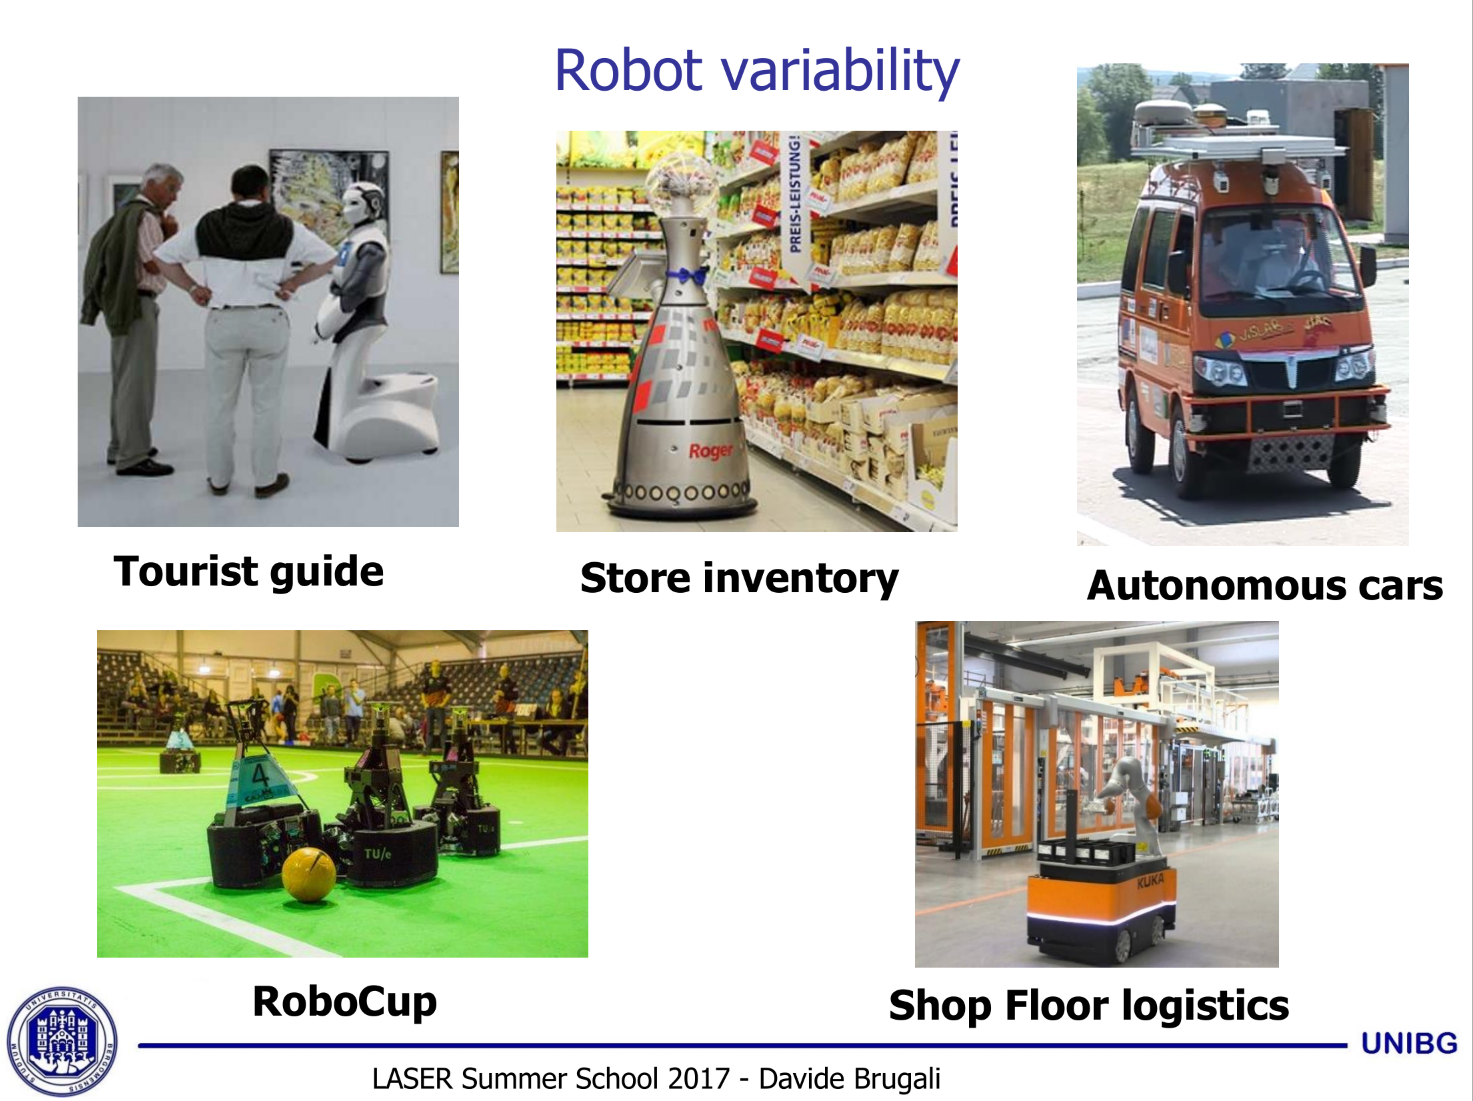
\includegraphics[width=0.9\textwidth]{brugali1.png}
		\end{center}
	\end{frame}

	\begin{frame}
		\begin{center}
			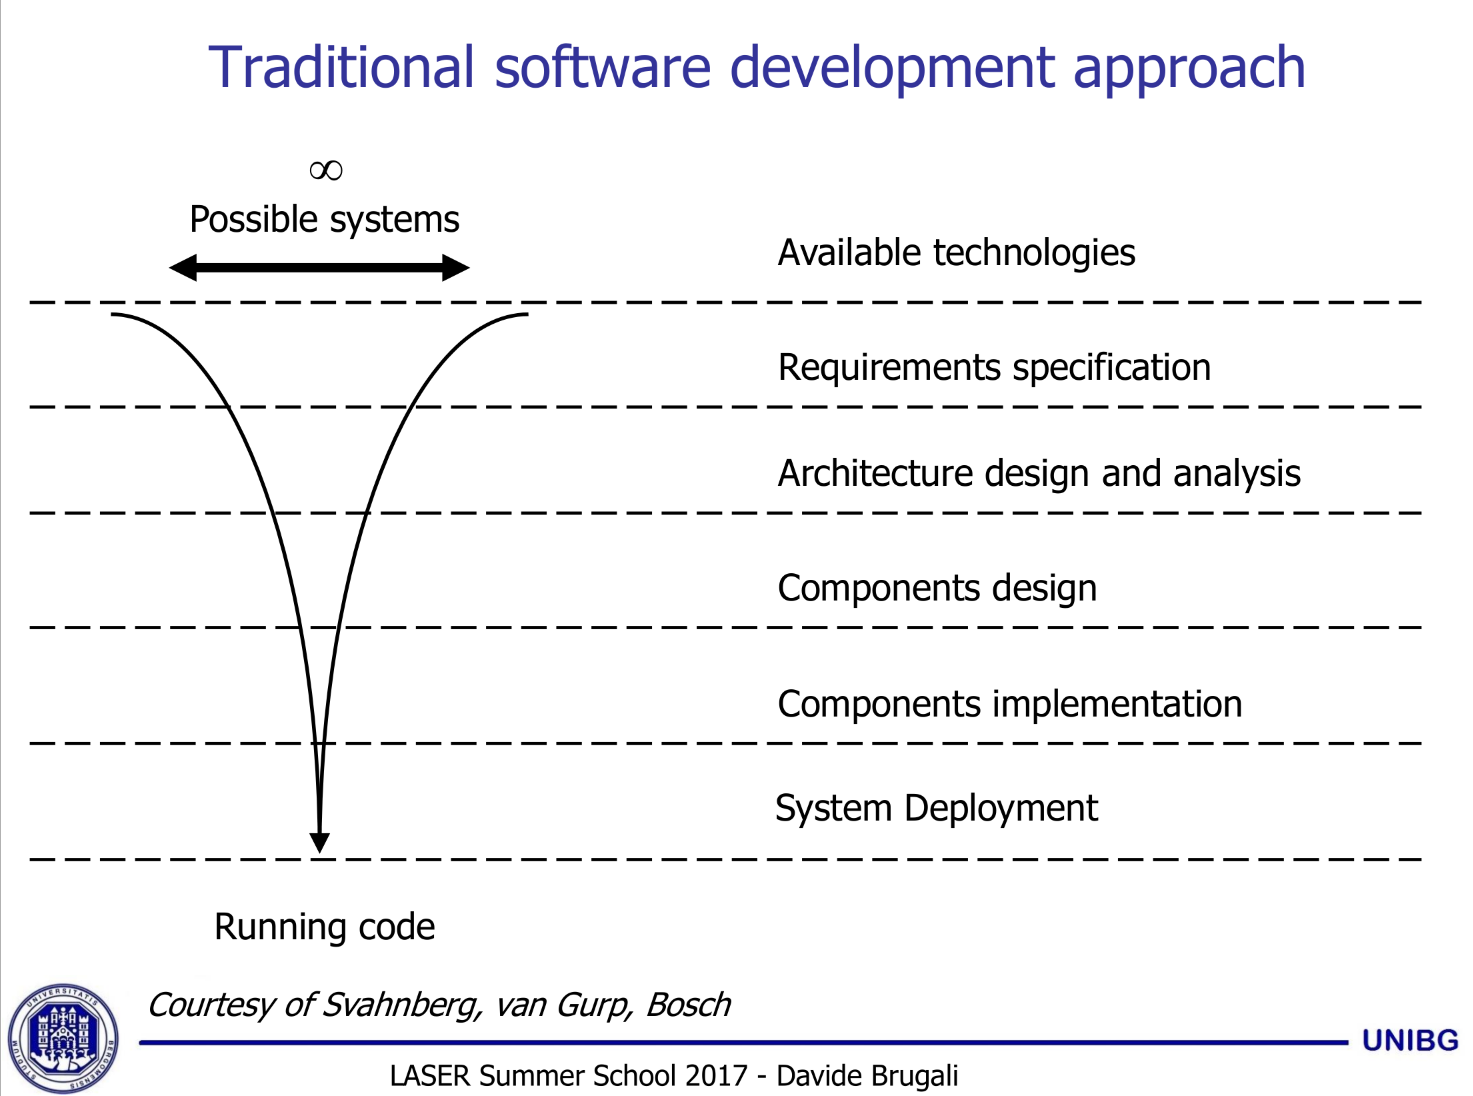
\includegraphics[width=0.9\textwidth]{brugali2.png}
		\end{center}
	\end{frame}

	\begin{frame}
		\begin{center}
			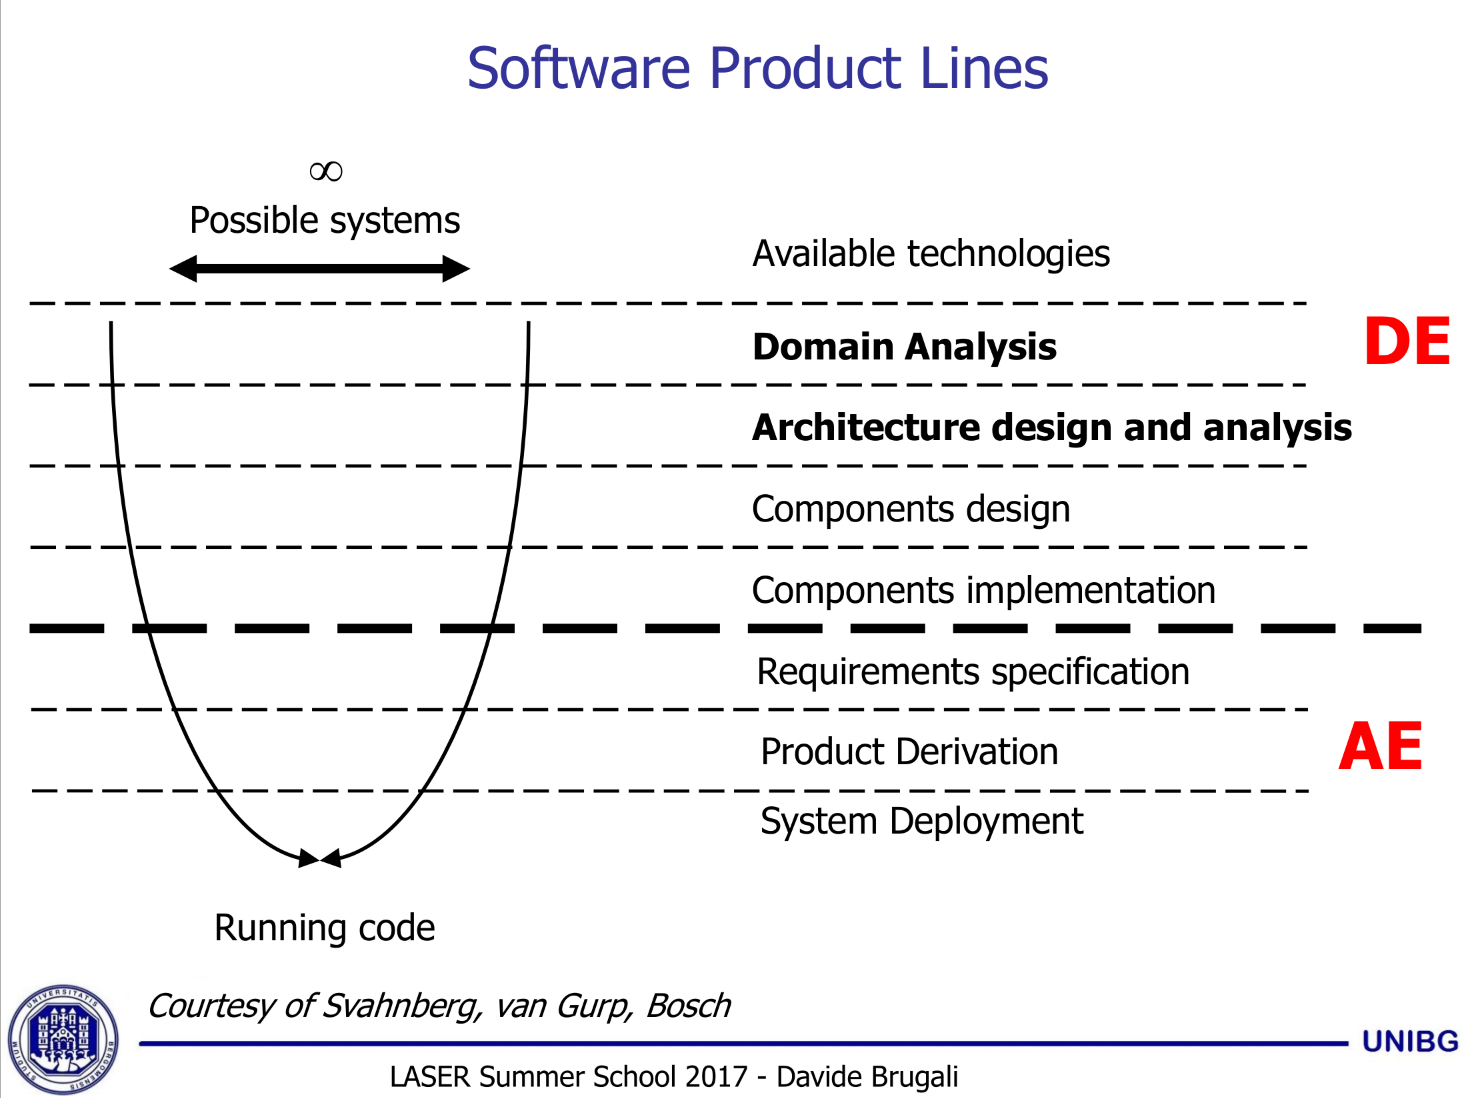
\includegraphics[width=0.9\textwidth]{brugali3.png}
		\end{center}
	\end{frame}

	\begin{frame}
		\begin{center}
			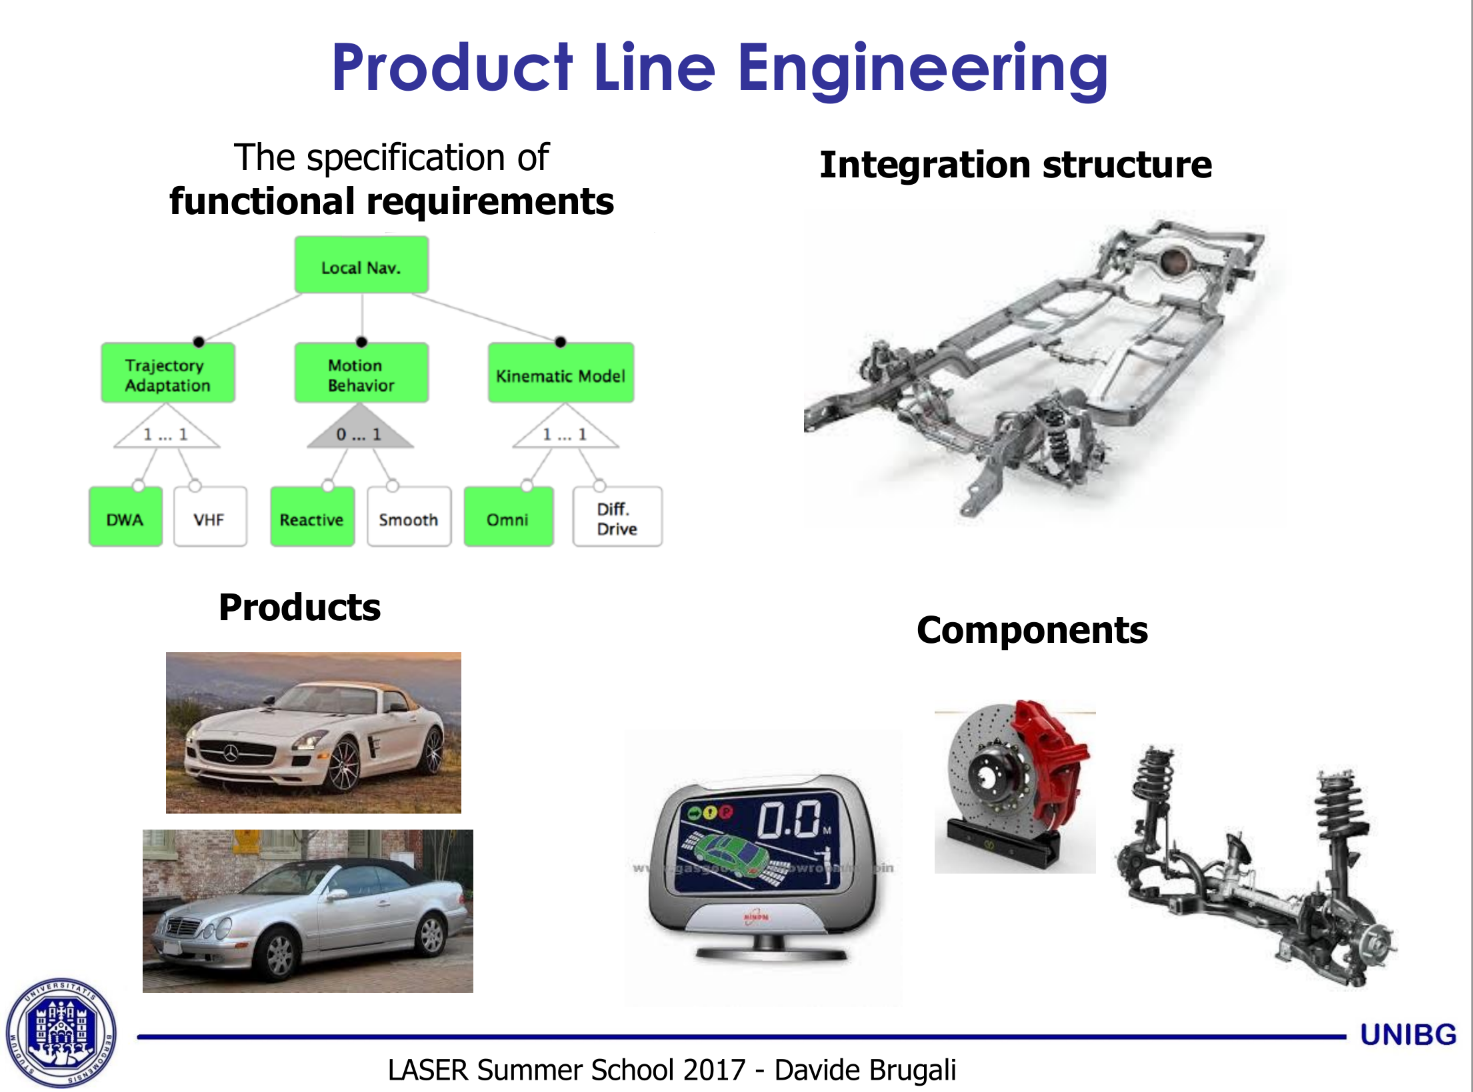
\includegraphics[width=0.9\textwidth]{brugali4.png}
		\end{center}
	\end{frame}

	\begin{frame}
		\begin{center}
			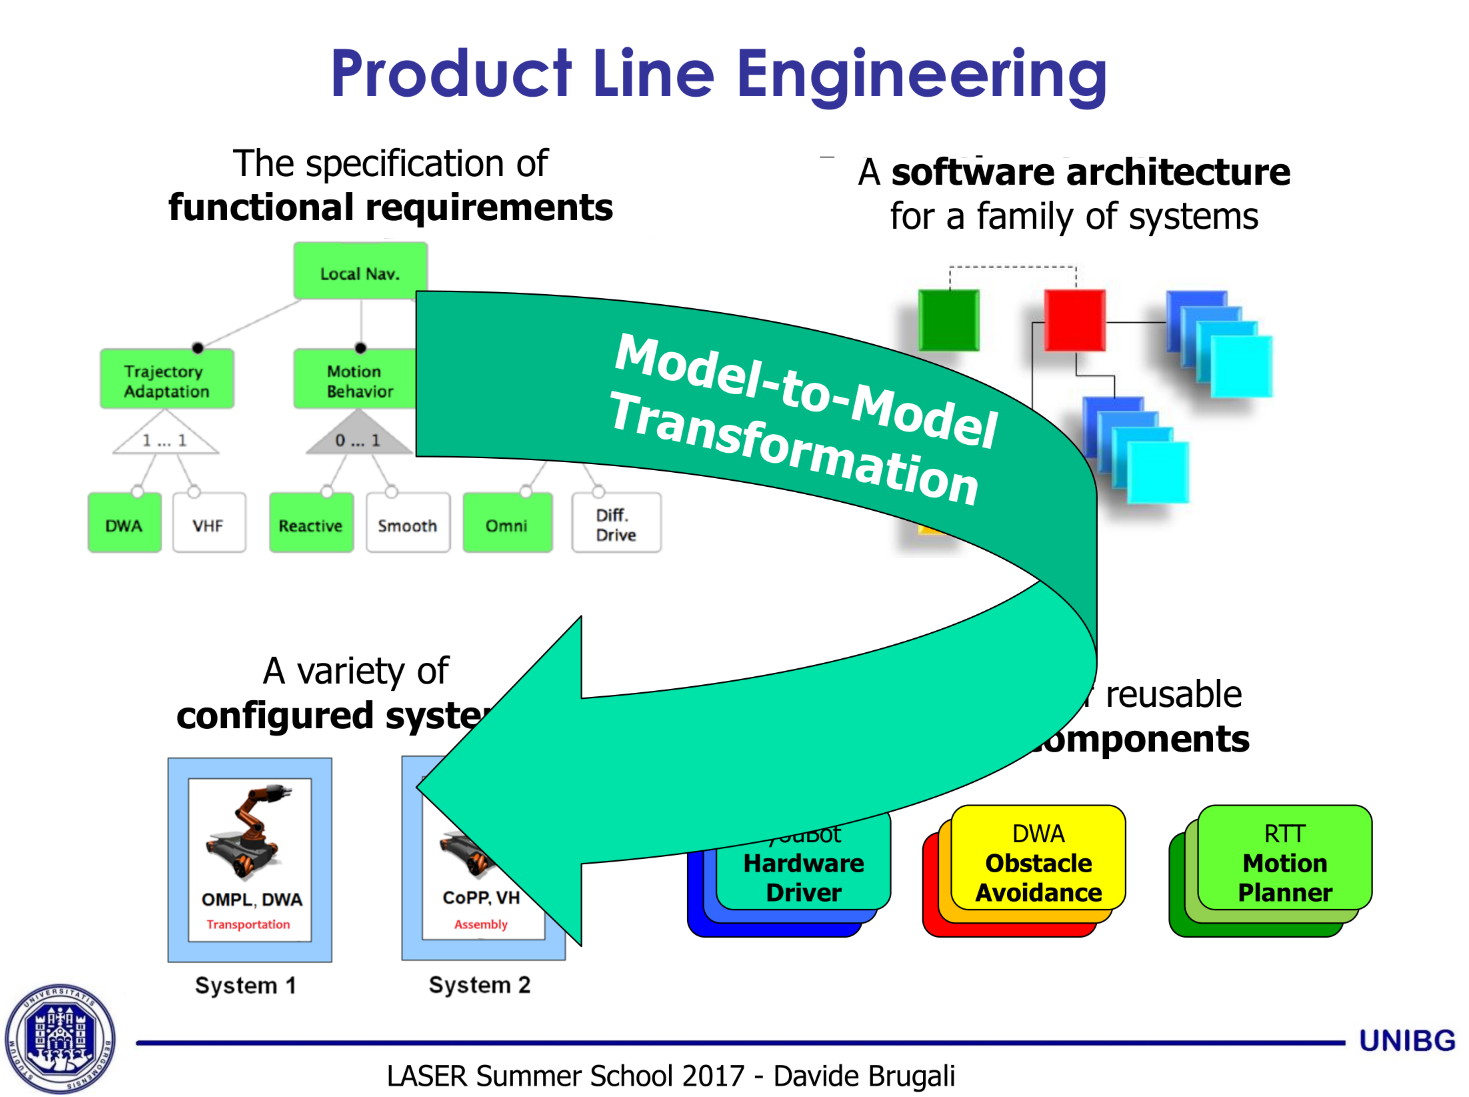
\includegraphics[width=0.9\textwidth]{brugali5.png}
		\end{center}
	\end{frame}

	\begin{frame}
		\begin{center}
			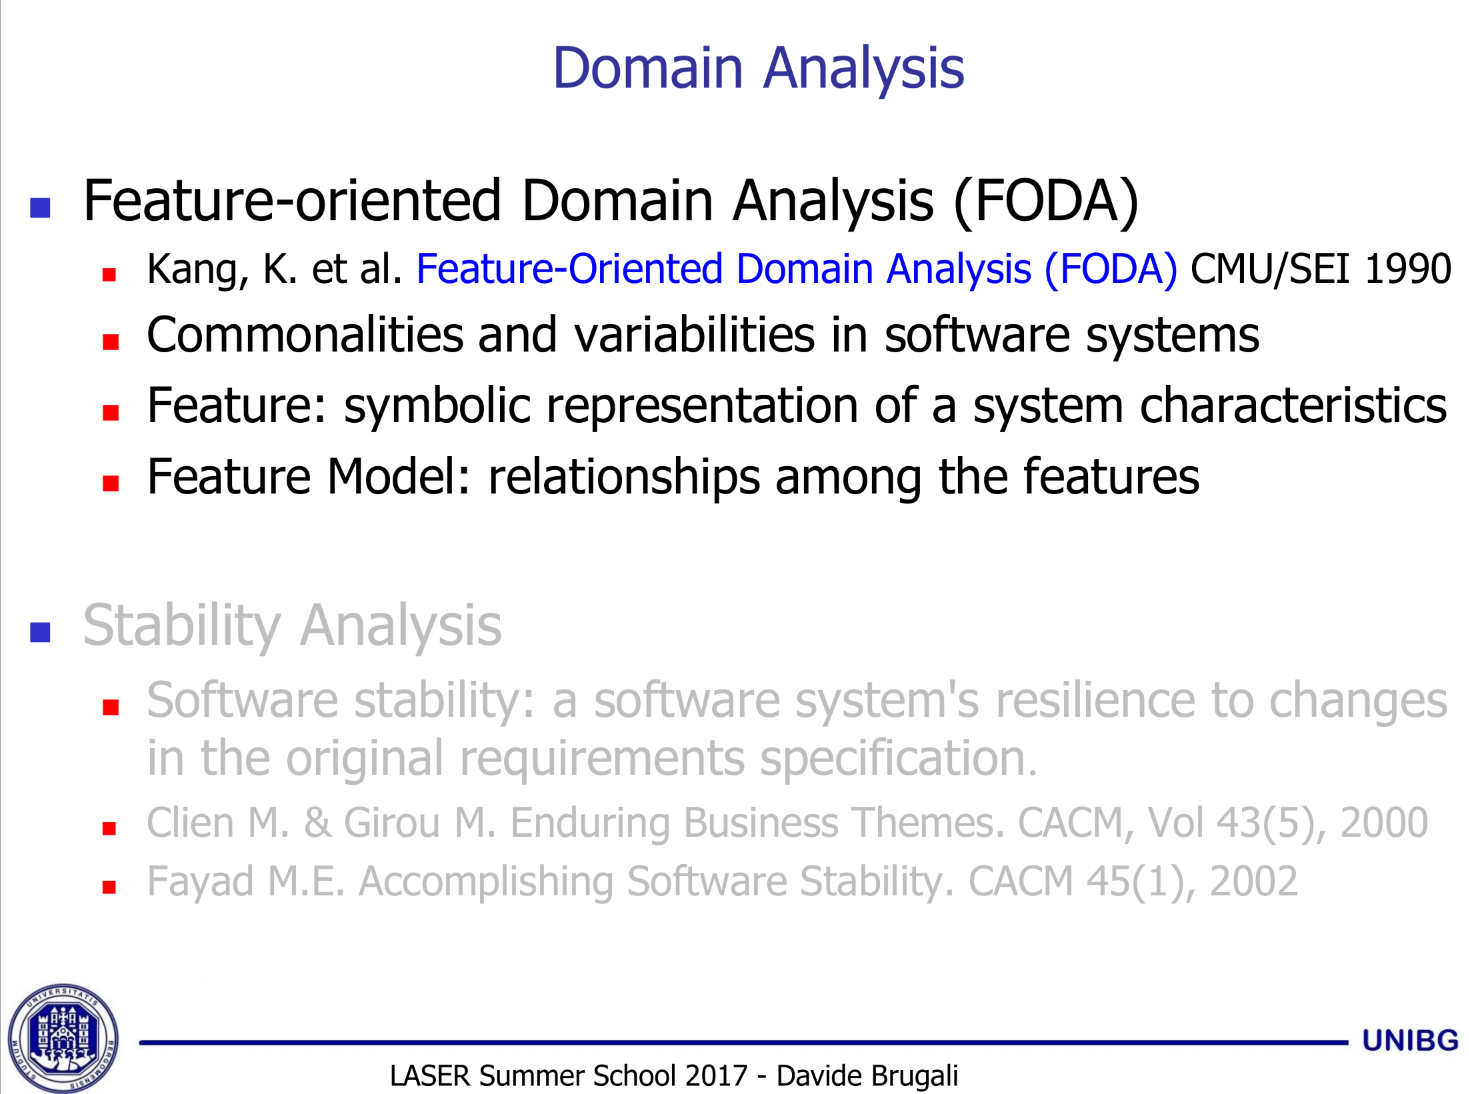
\includegraphics[width=0.9\textwidth]{brugali6.png}
		\end{center}
	\end{frame}

	\begin{frame}
		\begin{center}
			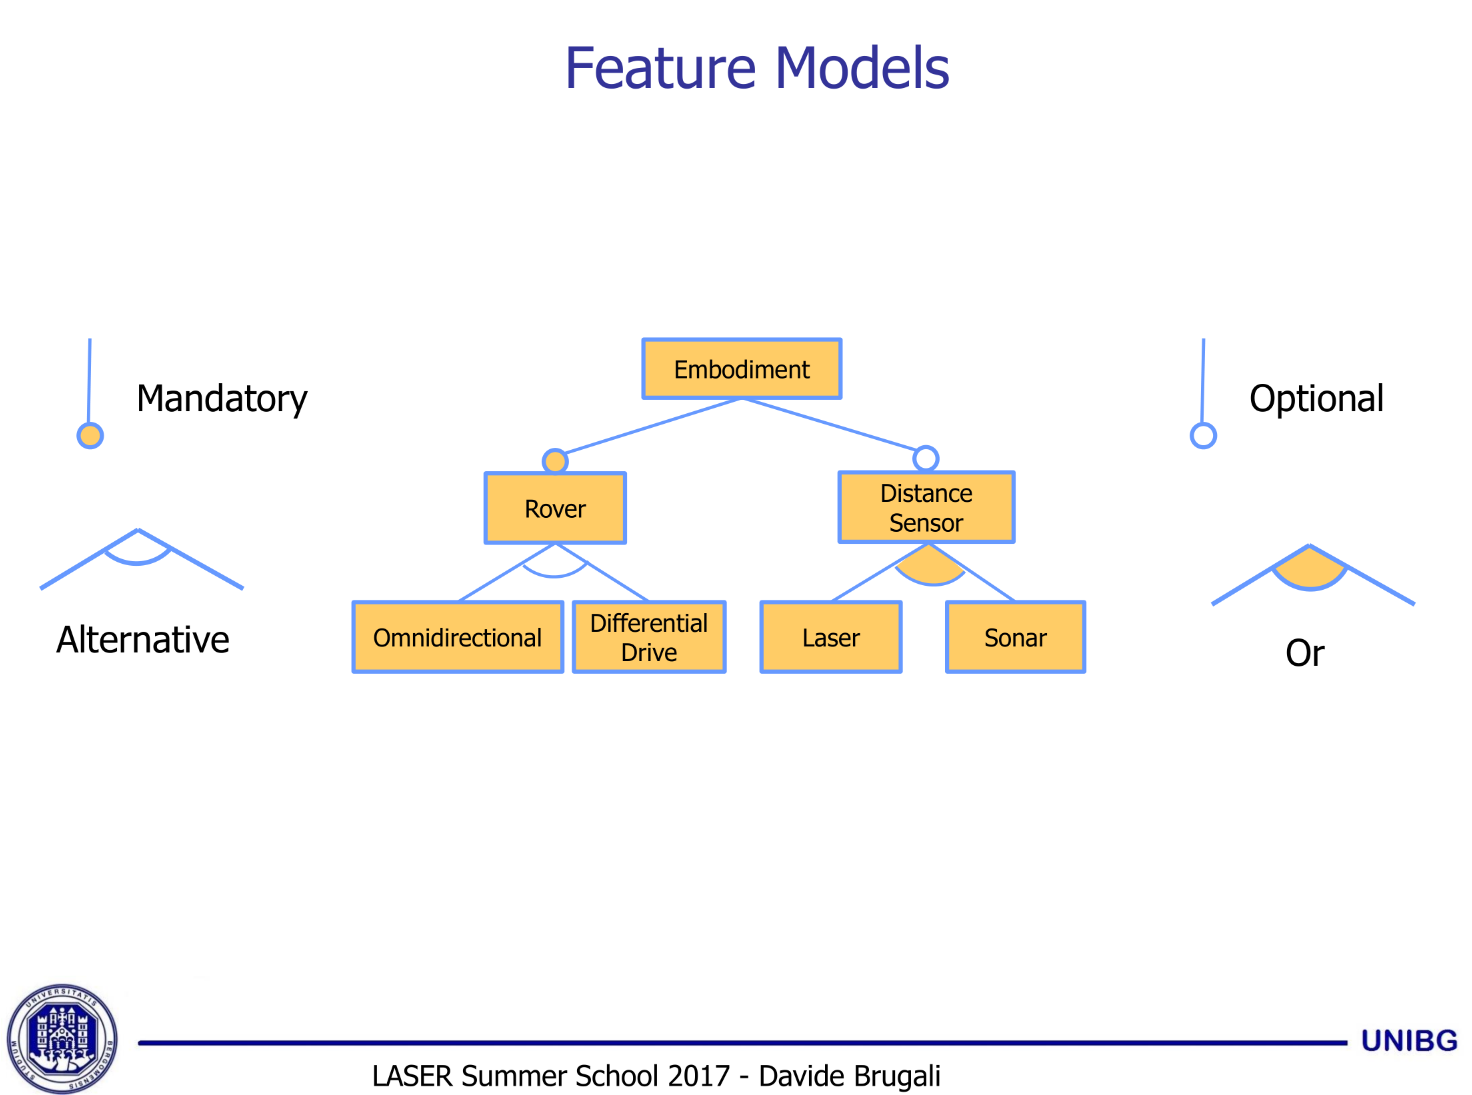
\includegraphics[width=0.9\textwidth]{brugali7.png}
		\end{center}
	\end{frame}

	\begin{frame}
		\begin{center}
			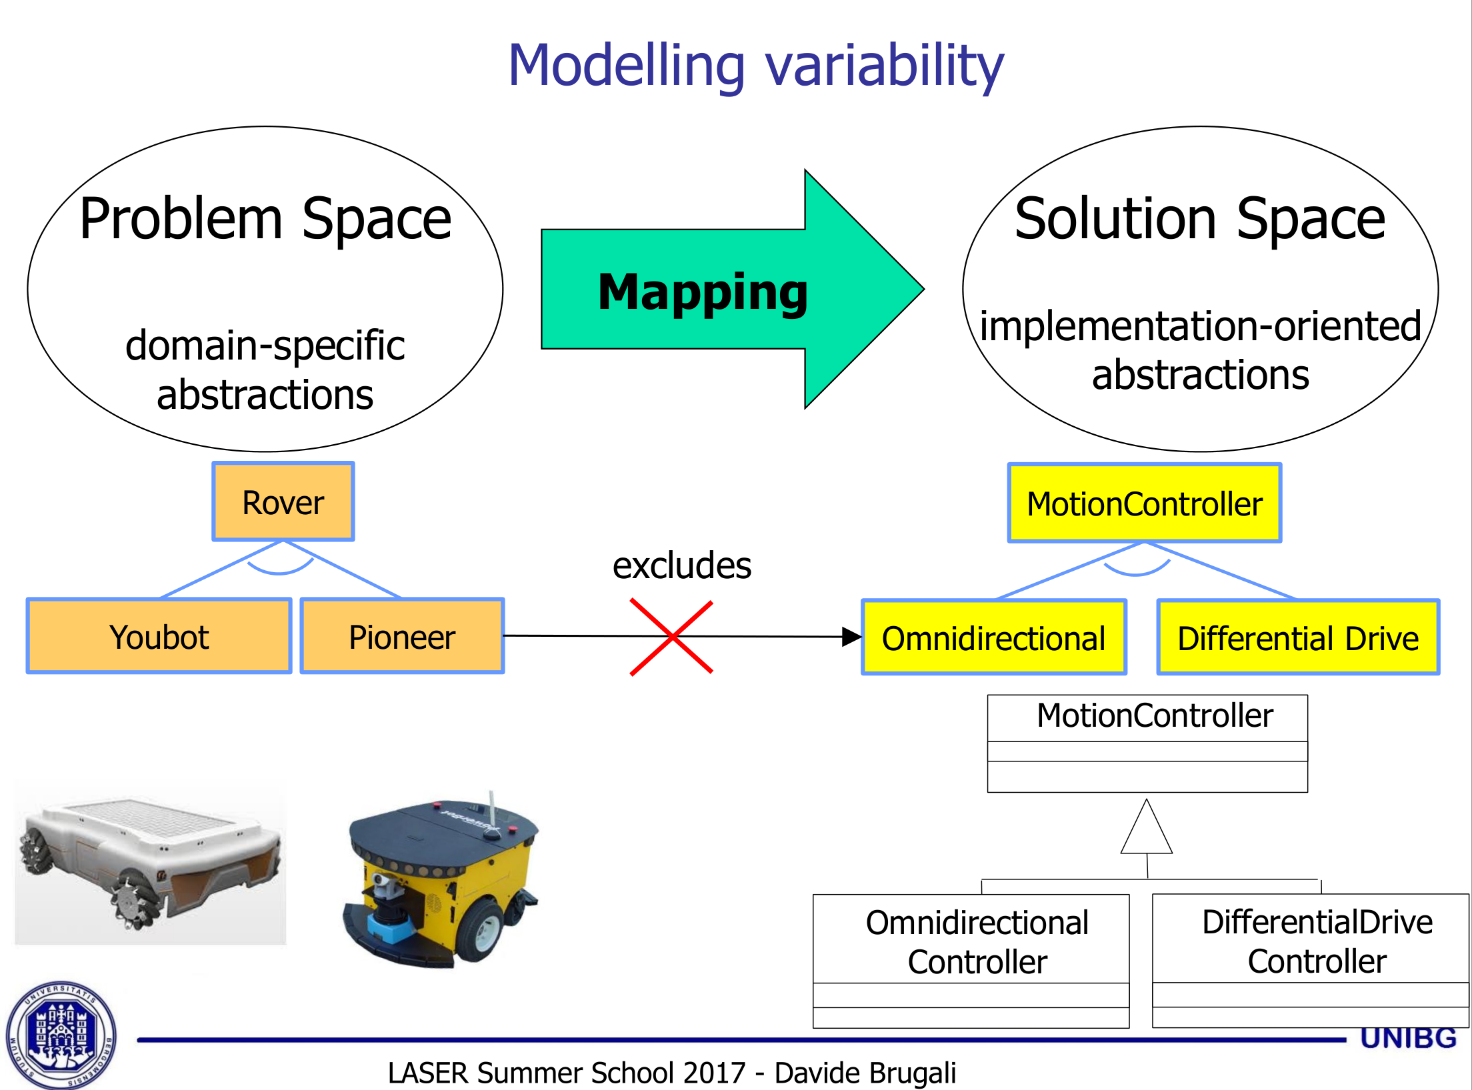
\includegraphics[width=0.9\textwidth]{brugali8.png}
		\end{center}
	\end{frame}

	\begin{frame}
		\begin{center}
			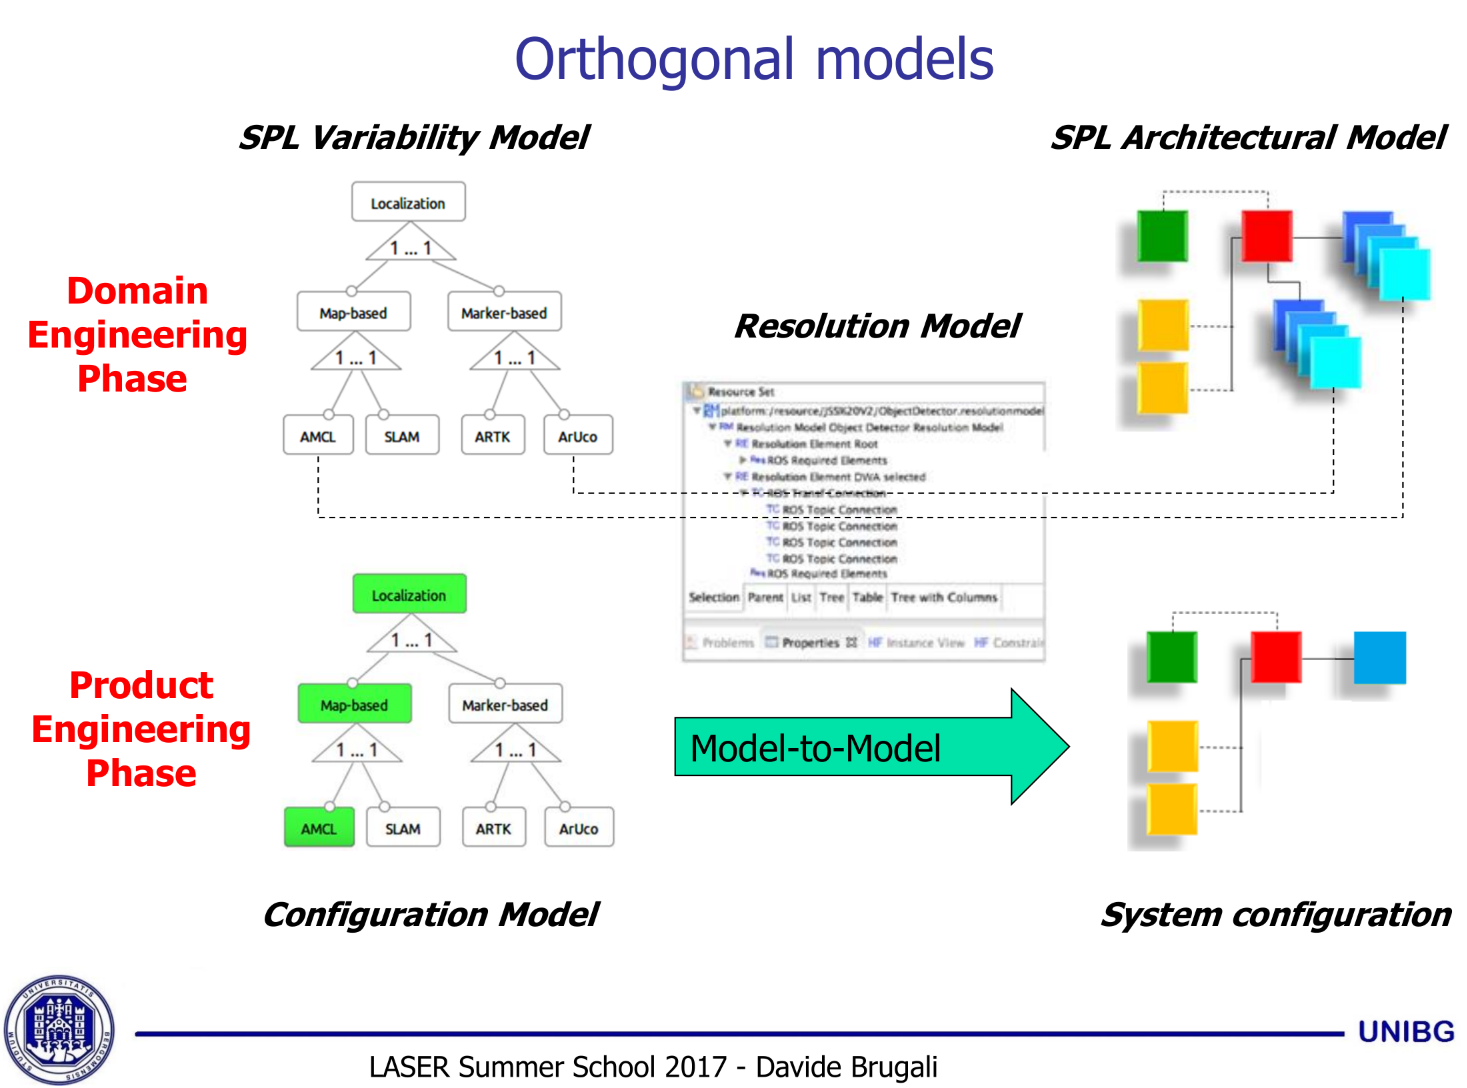
\includegraphics[width=0.9\textwidth]{brugali9.png}
		\end{center}
	\end{frame}

	\begin{frame}
		\begin{center}
			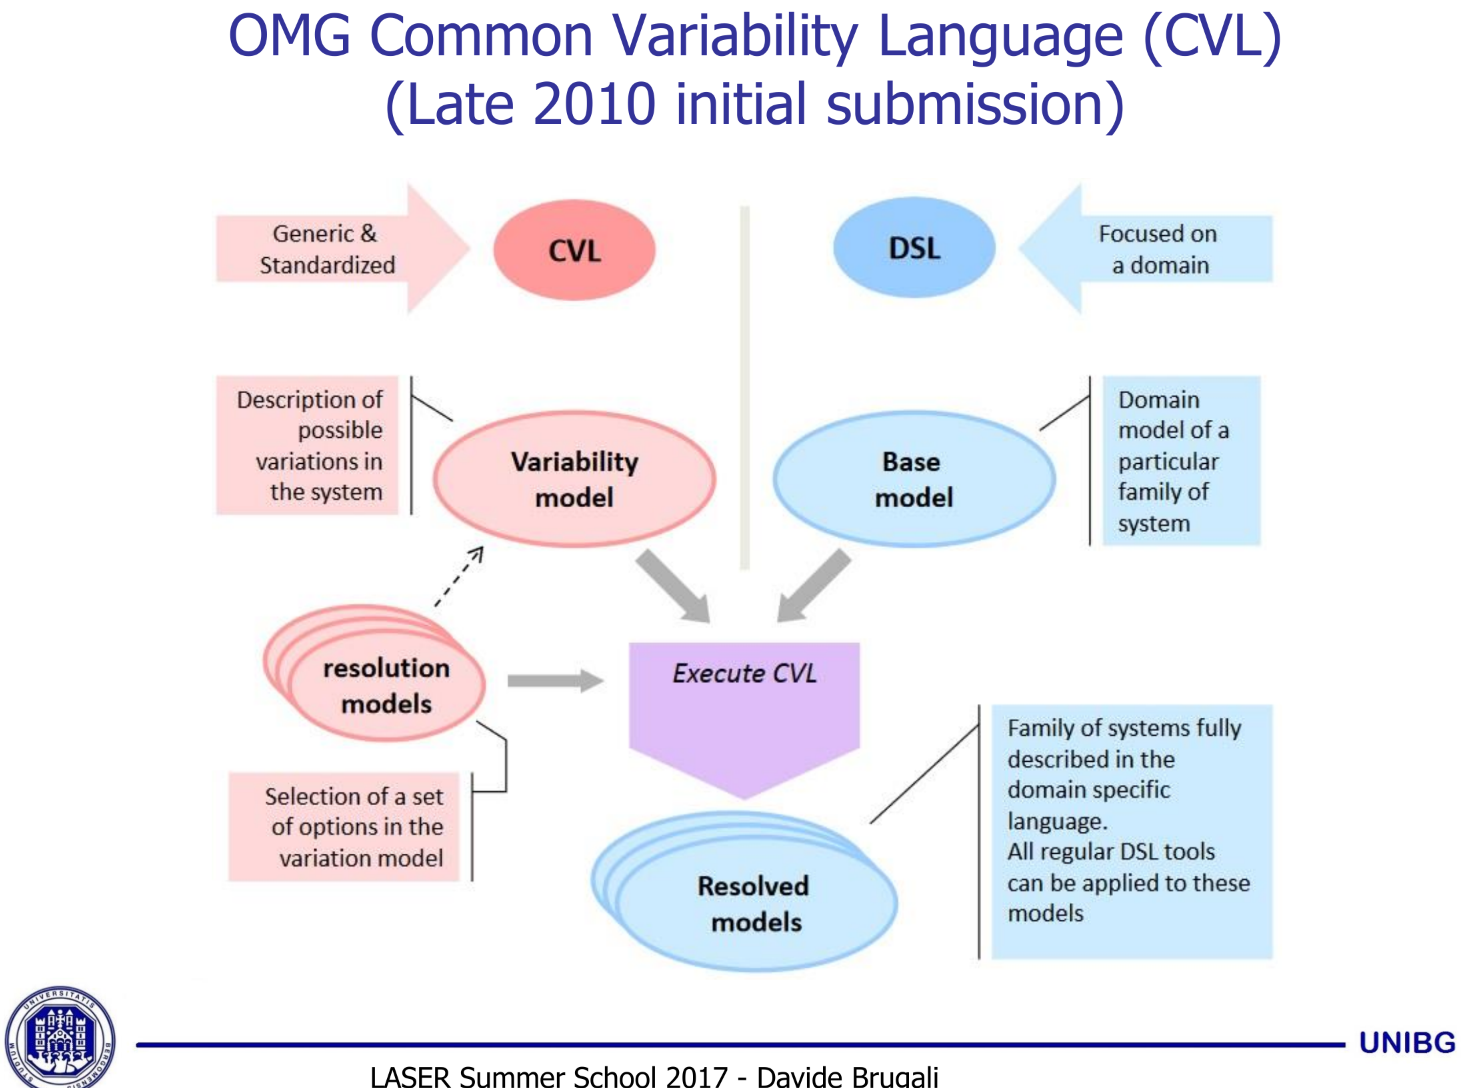
\includegraphics[width=0.9\textwidth]{brugali10.png}
		\end{center}
	\end{frame}

	\begin{frame}
		\begin{center}
			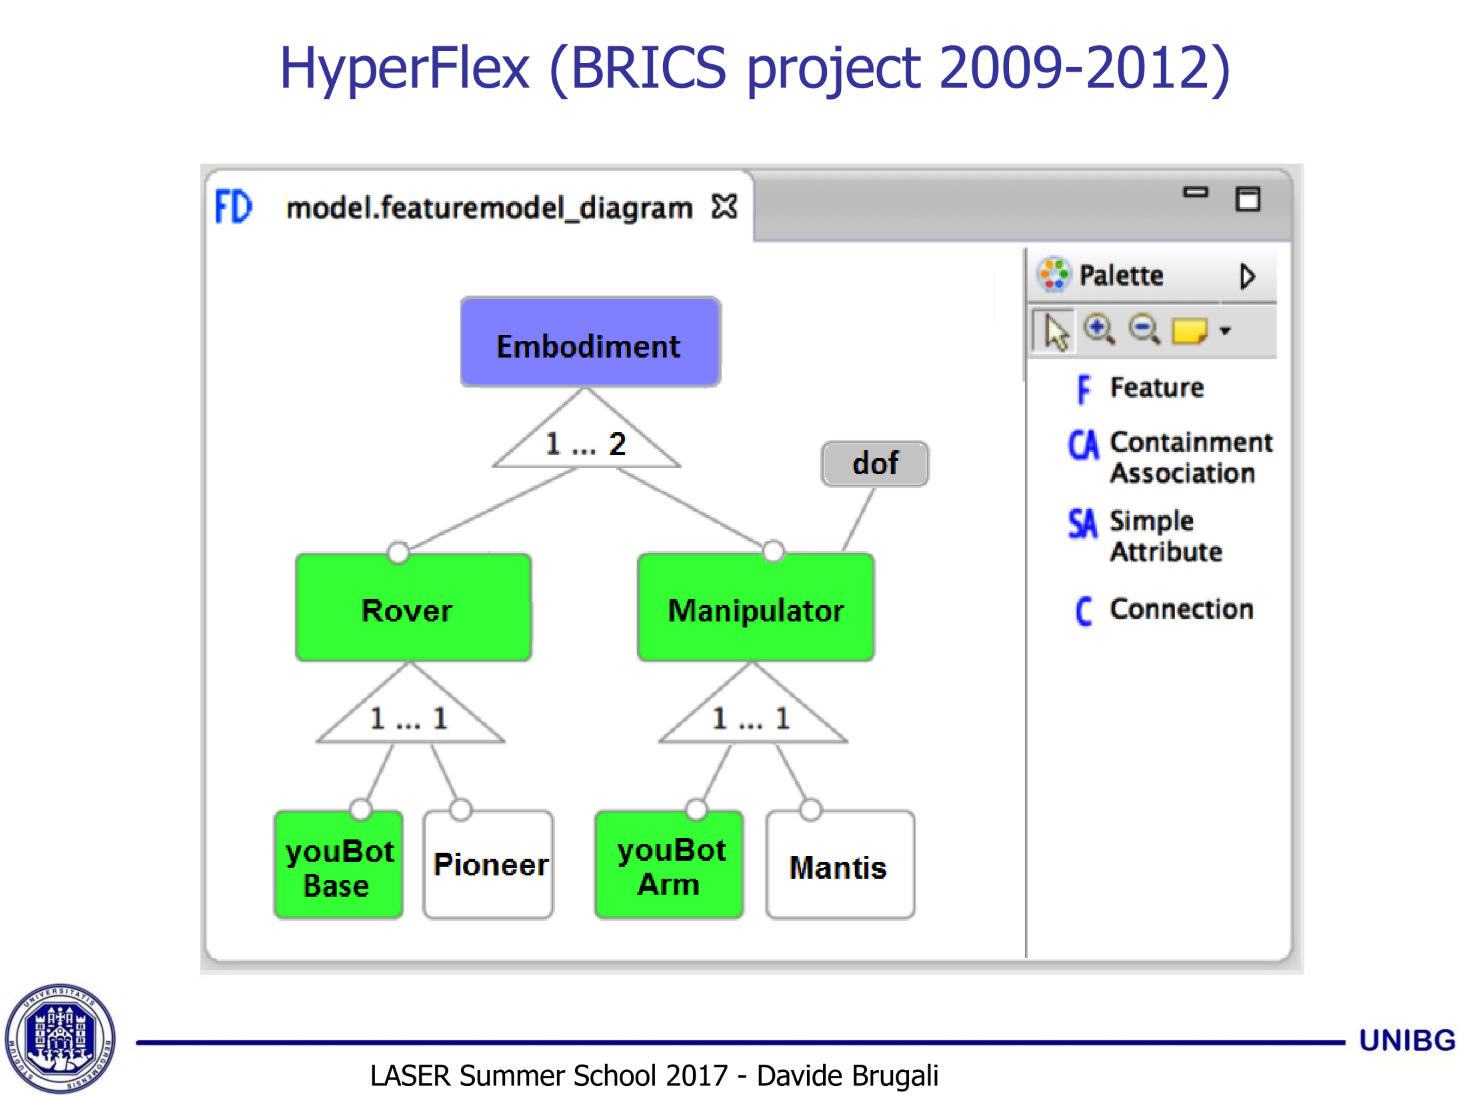
\includegraphics[width=0.9\textwidth]{brugali11.png}
		\end{center}
	\end{frame}

	\begin{frame}
		\begin{center}
			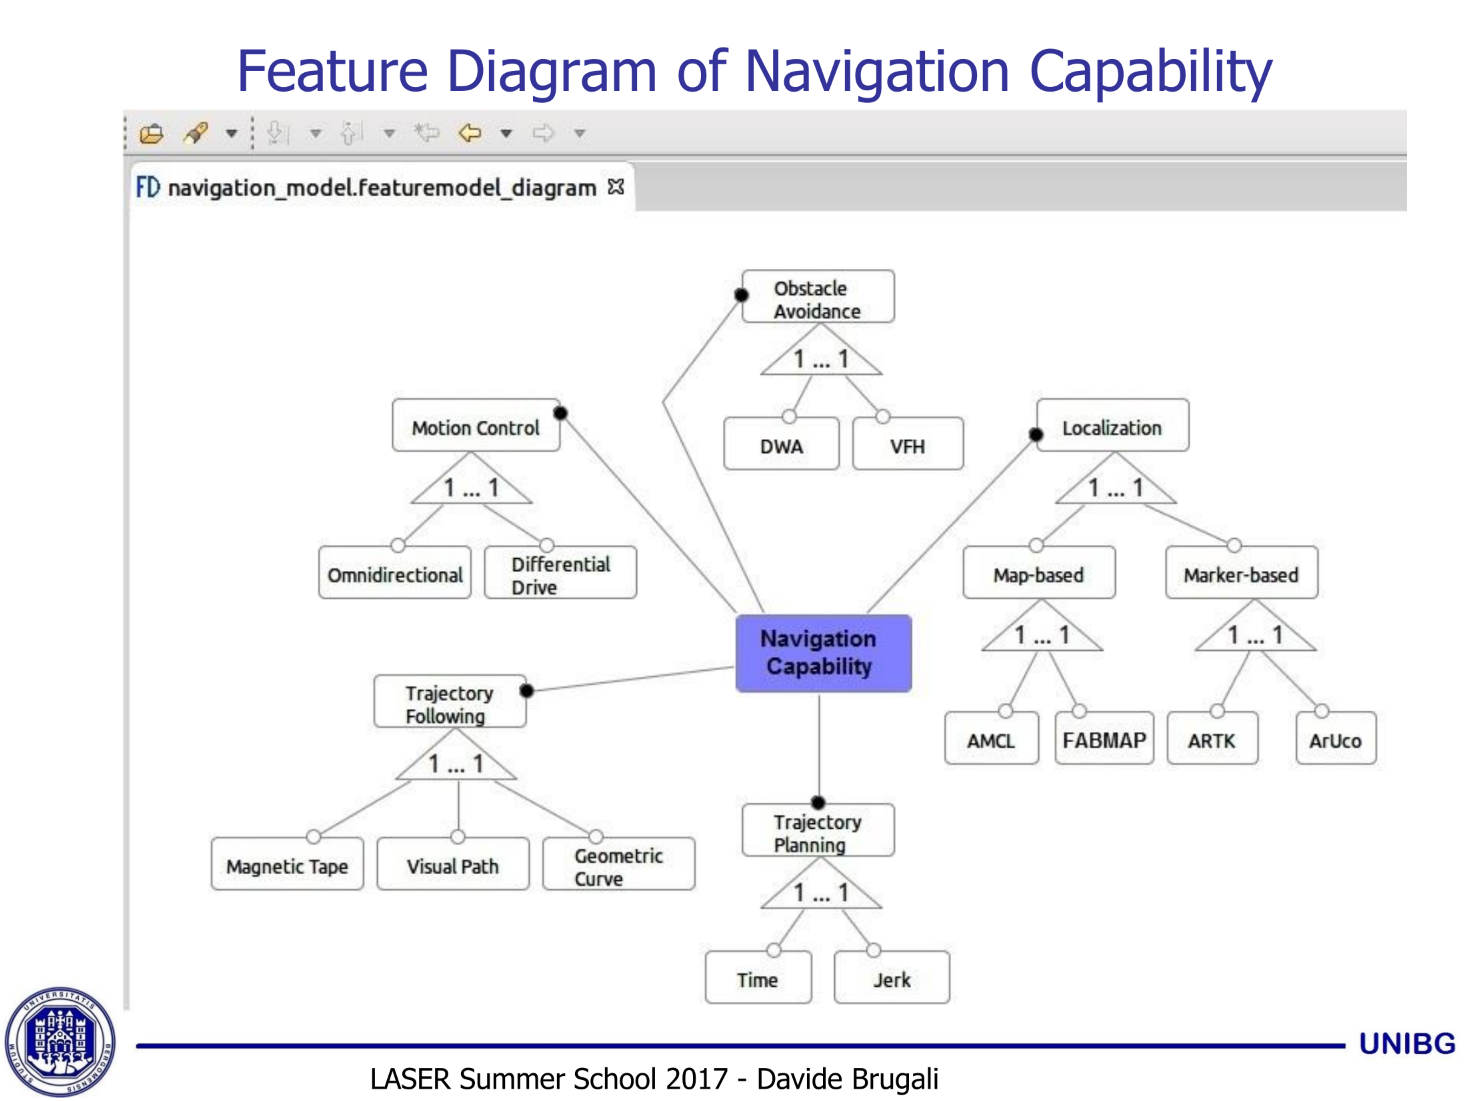
\includegraphics[width=0.9\textwidth]{brugali12.png}
		\end{center}
	\end{frame}

	\begin{frame}
		\begin{center}
			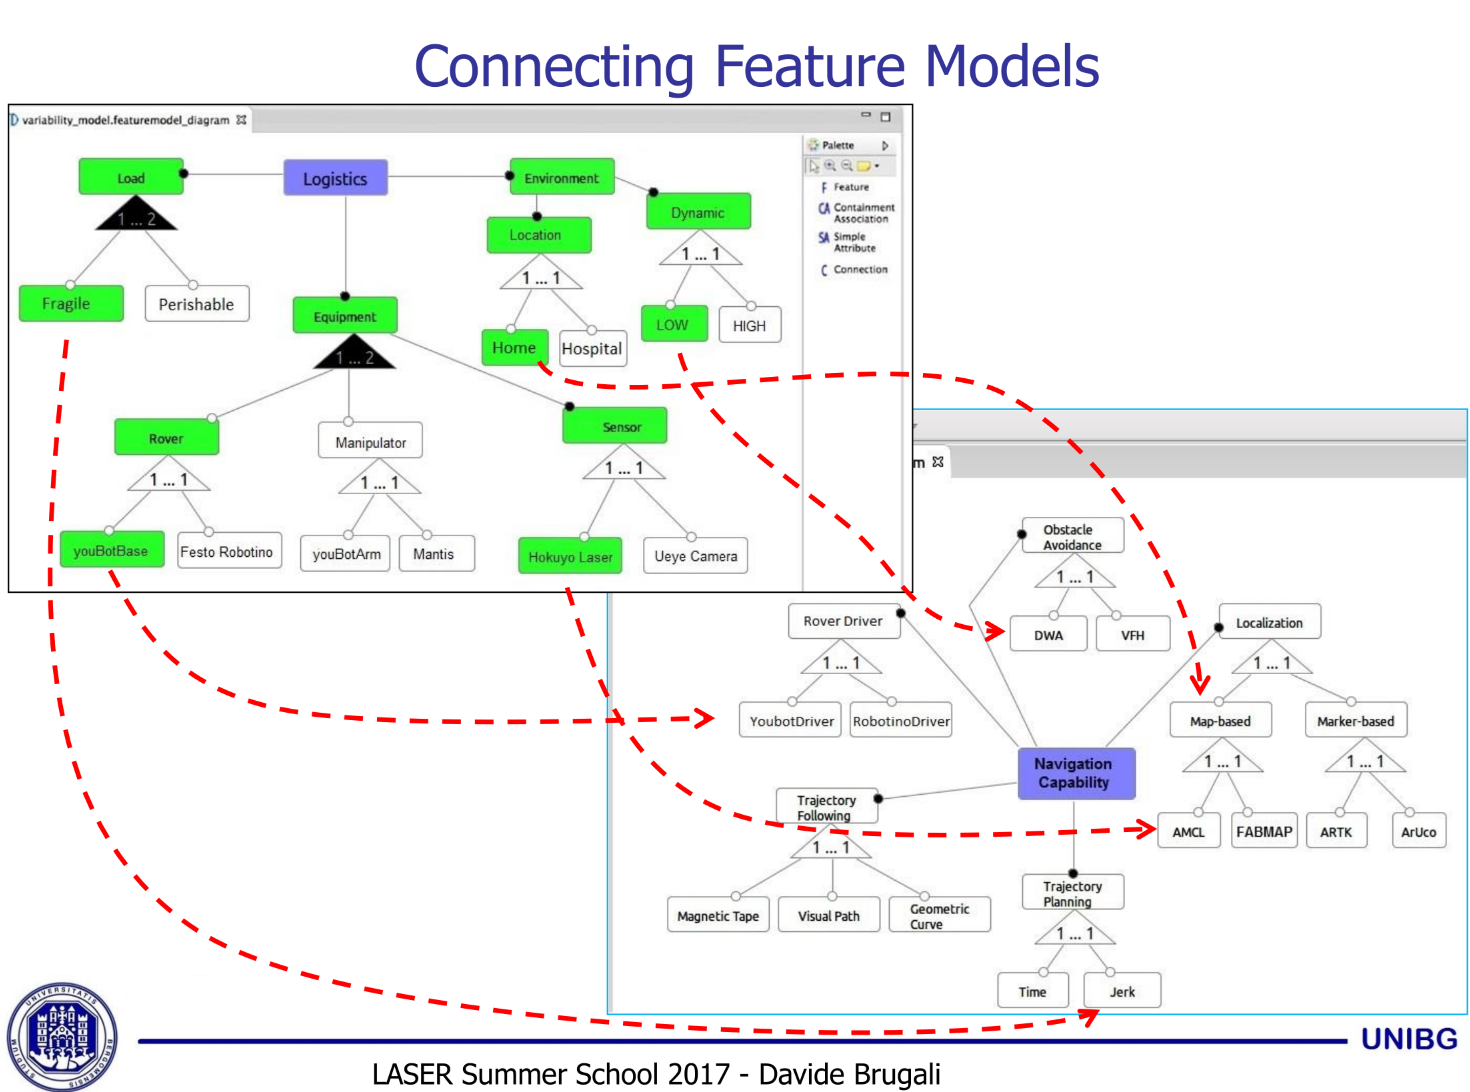
\includegraphics[width=0.9\textwidth]{brugali13.png}
		\end{center}
	\end{frame}

	\begin{frame}
		\begin{center}
			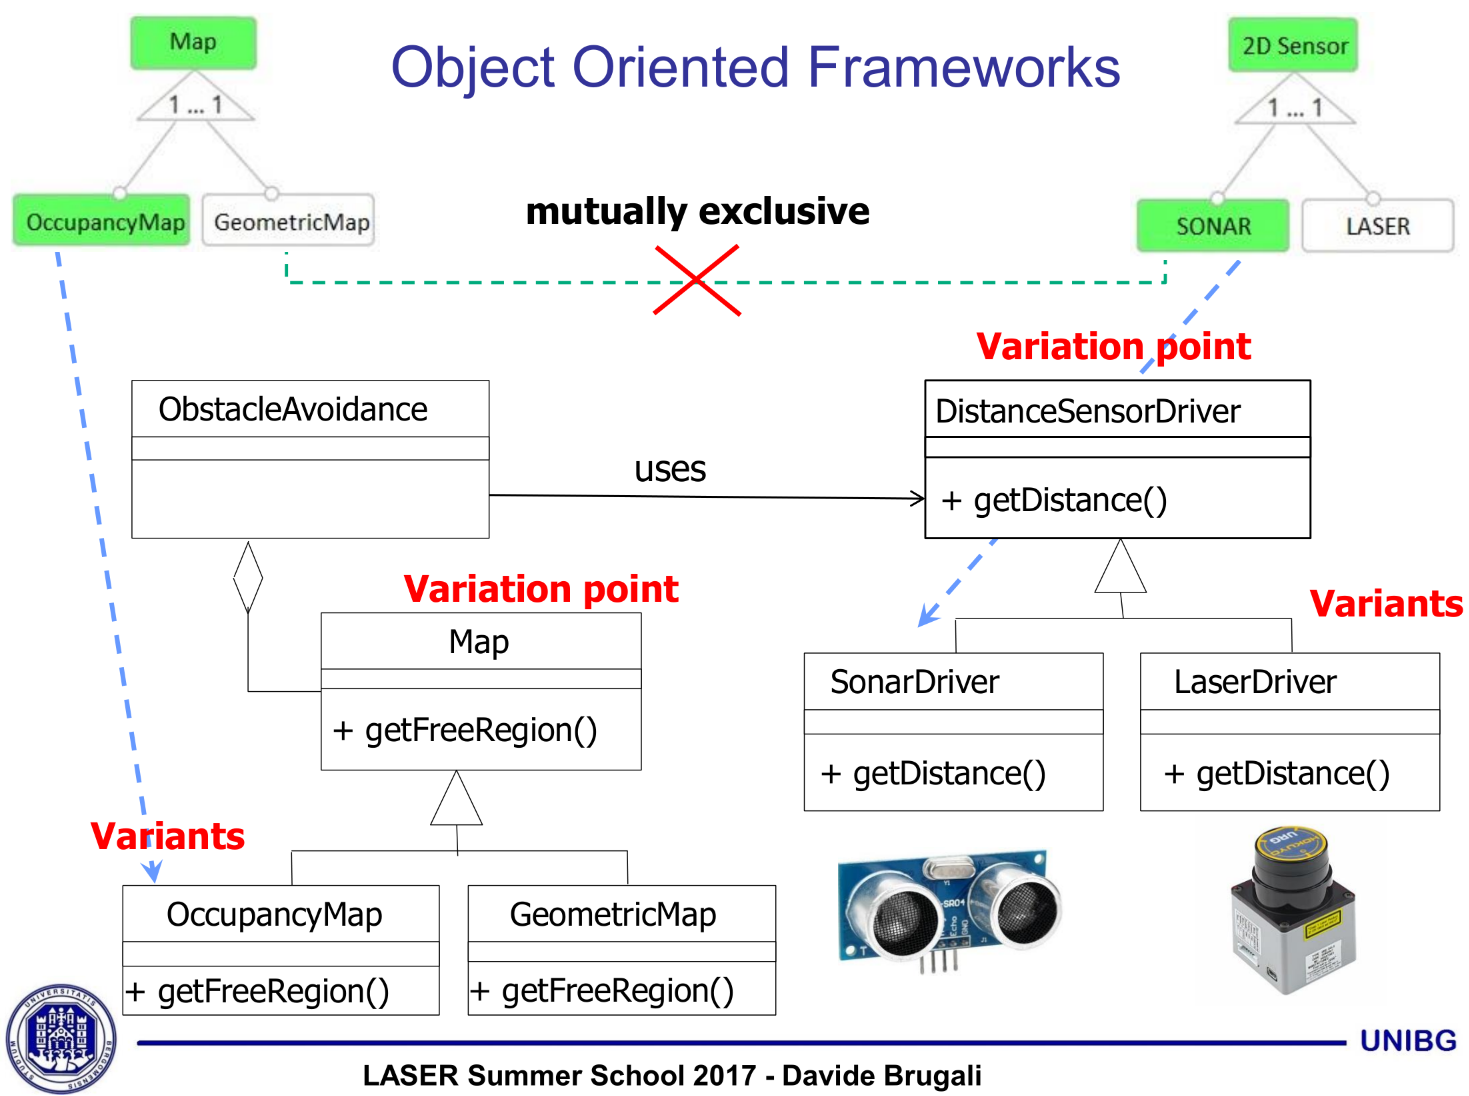
\includegraphics[width=0.9\textwidth]{brugali14.png}
		\end{center}
	\end{frame}

	\begin{frame}
		\begin{center}
			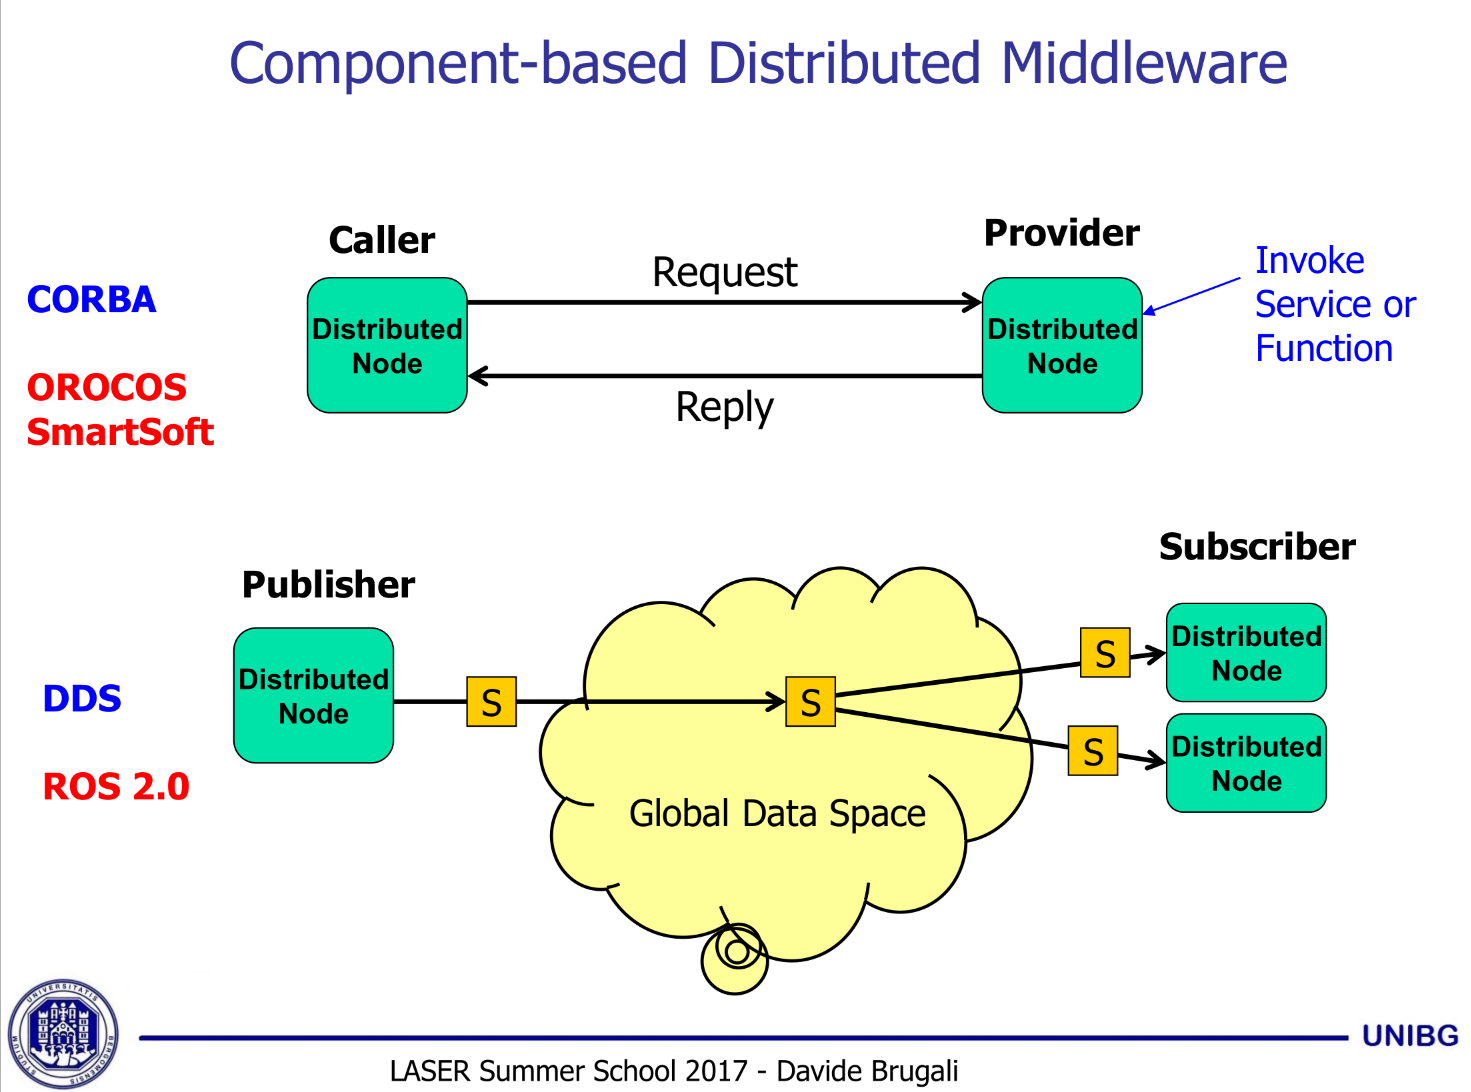
\includegraphics[width=0.9\textwidth]{brugali15.png}
		\end{center}
	\end{frame}

	\begin{frame}
		\begin{center}
			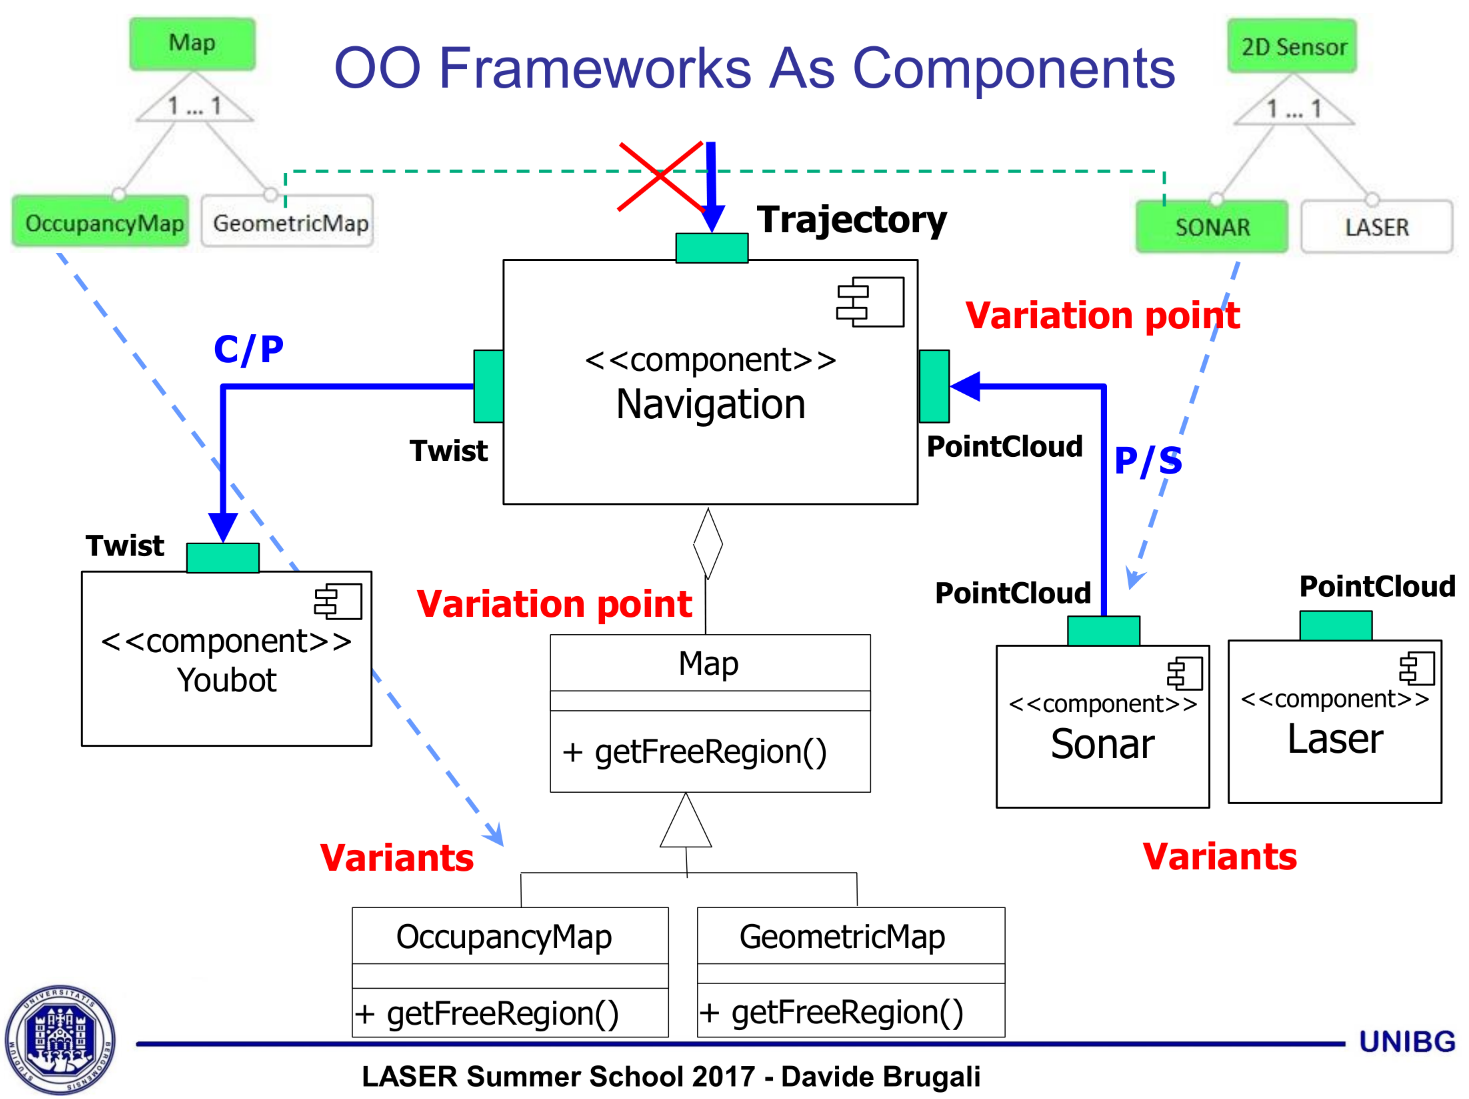
\includegraphics[width=0.9\textwidth]{brugali16.png}
		\end{center}
	\end{frame}

	\begin{frame}
		\begin{center}
			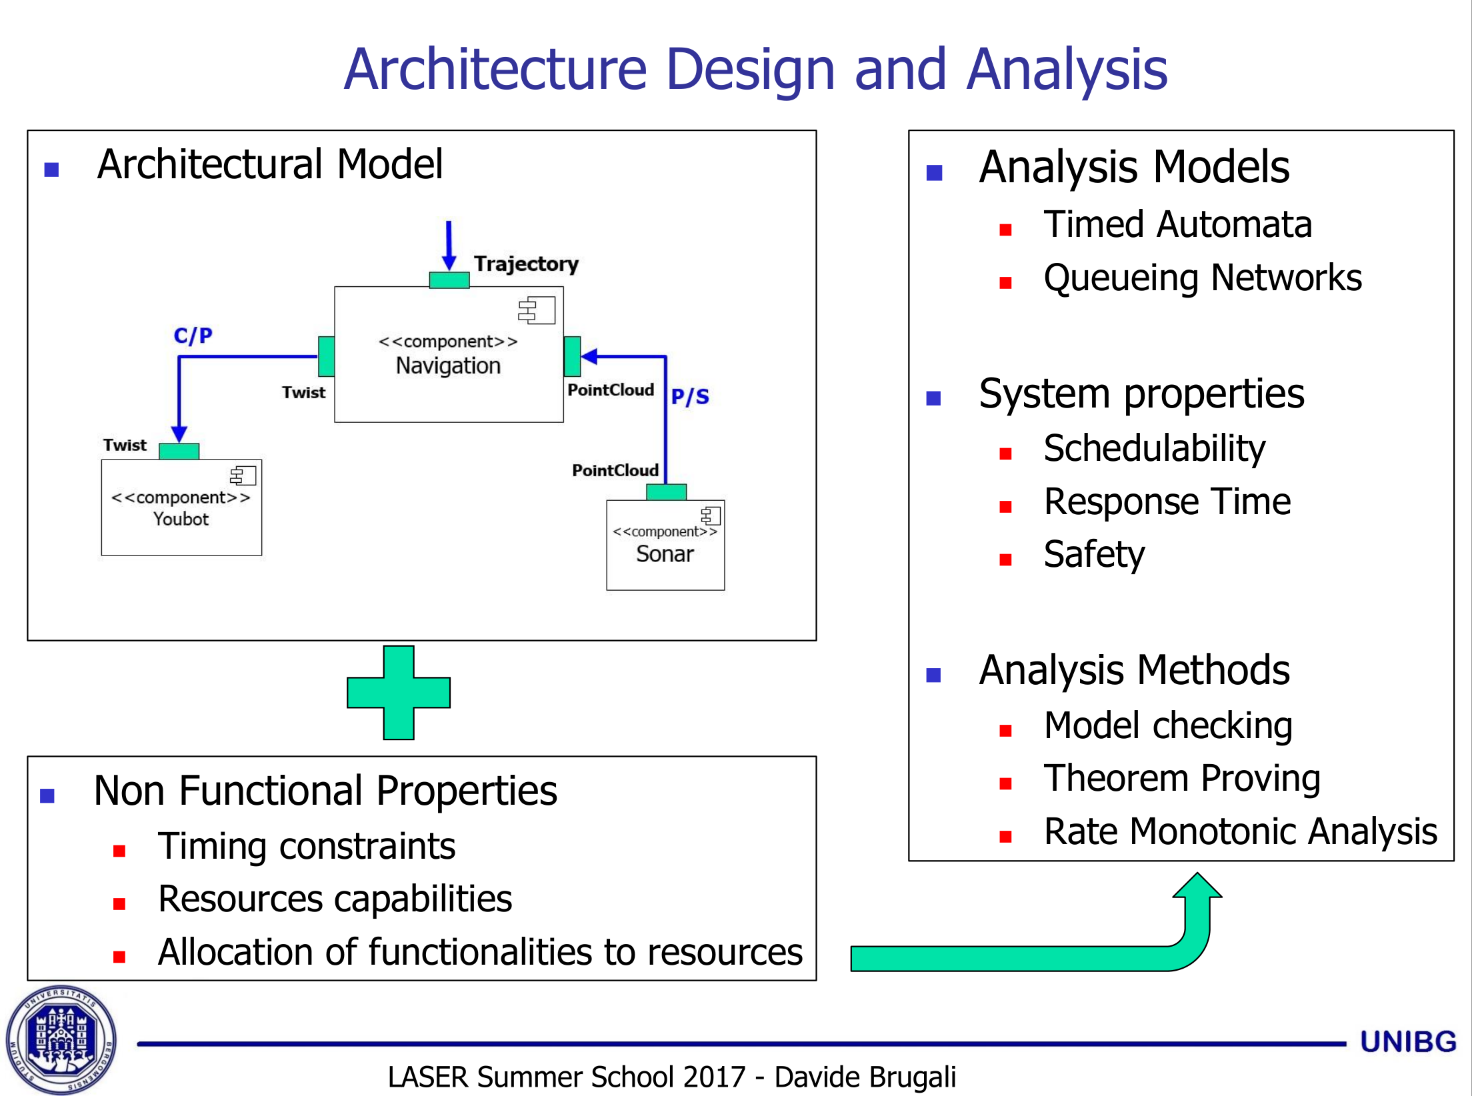
\includegraphics[width=0.9\textwidth]{brugali17.png}
		\end{center}
	\end{frame}

	\begin{frame}
		\begin{center}
			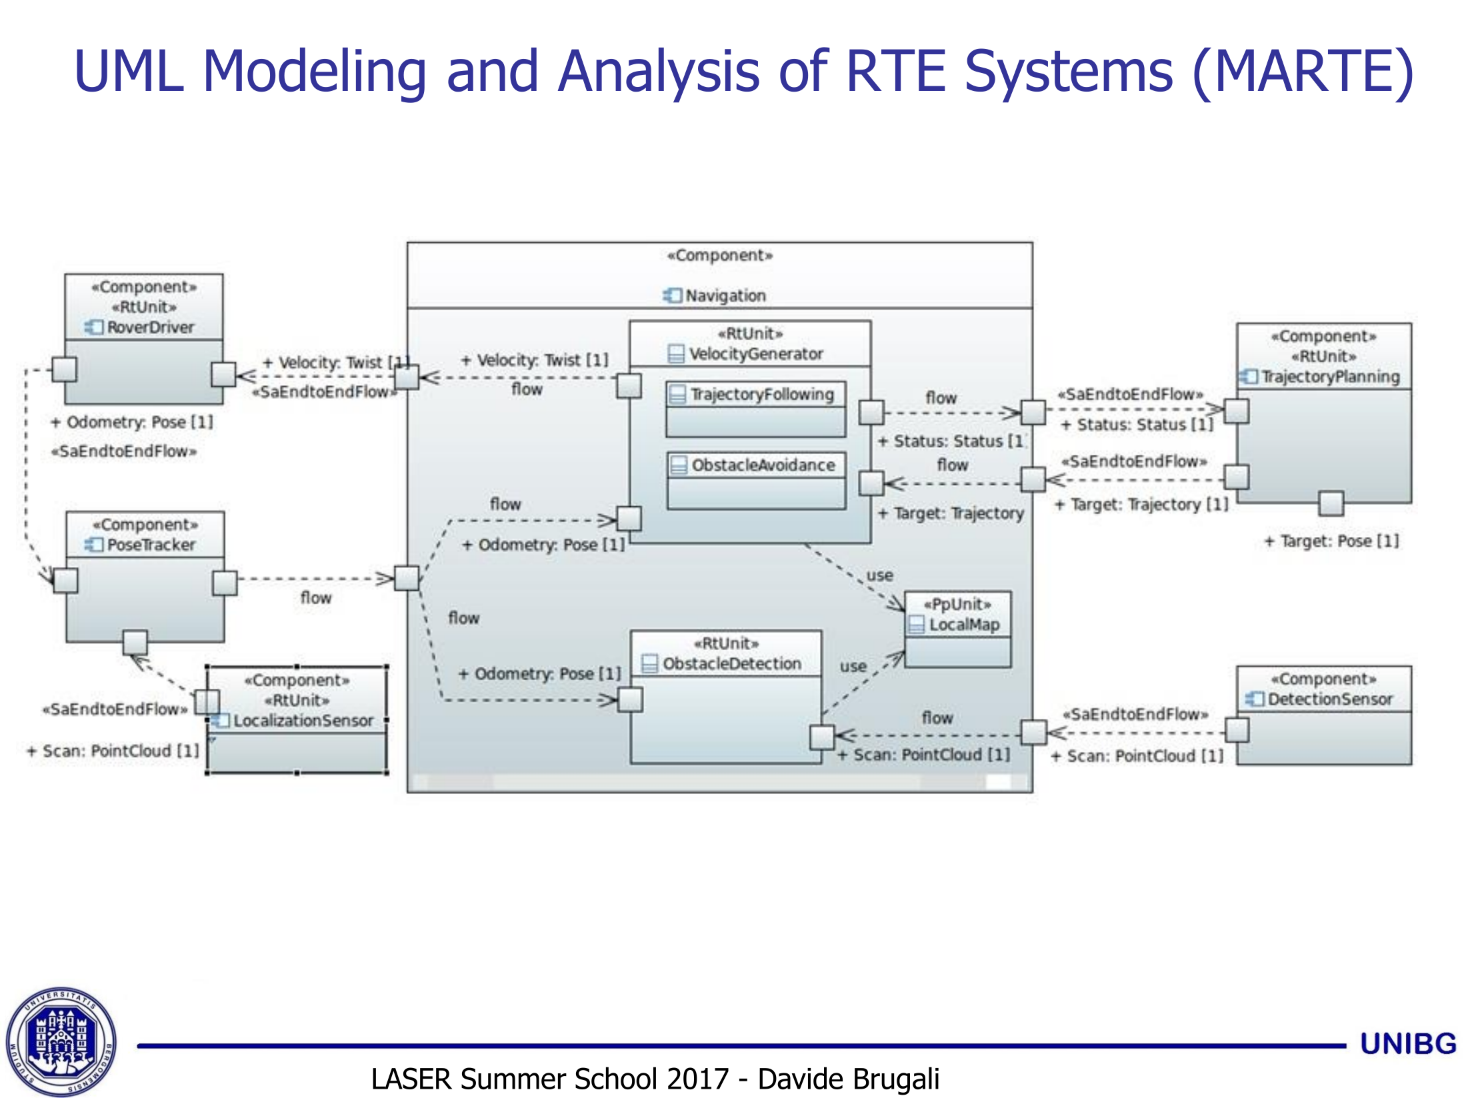
\includegraphics[width=0.9\textwidth]{brugali18.png}
		\end{center}
	\end{frame}

	\begin{frame}
		\begin{center}
			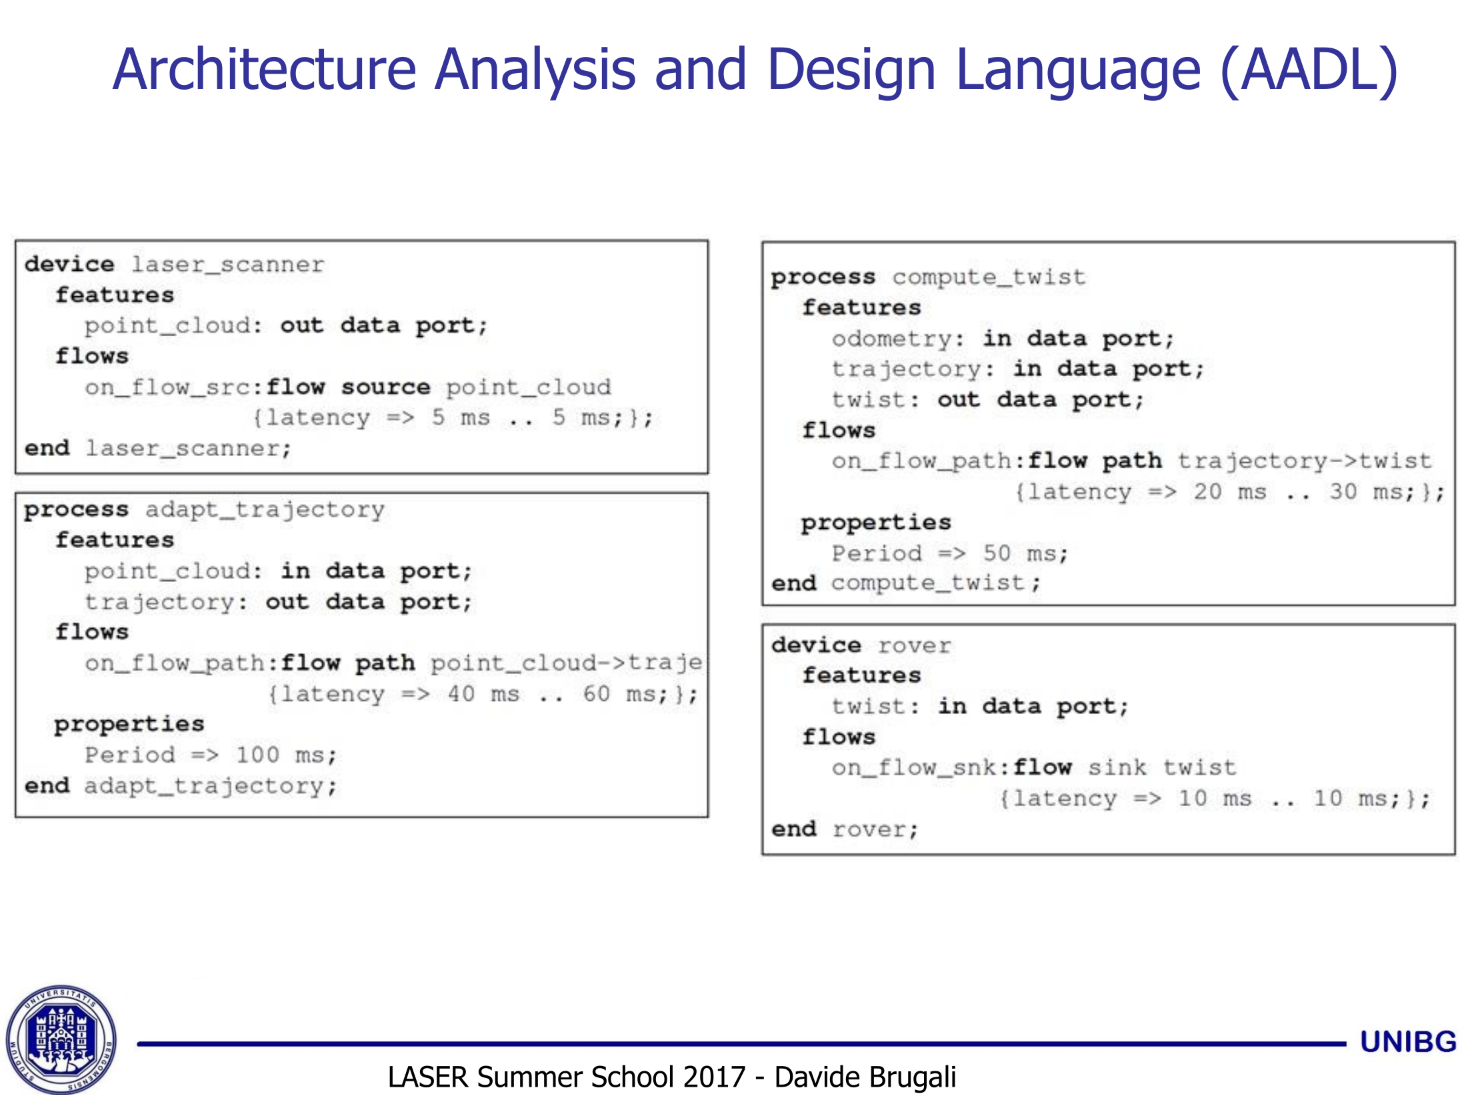
\includegraphics[width=0.9\textwidth]{brugali19.png}
		\end{center}
	\end{frame}

	\section{R. Gelin}

	\begin{frame}
		\begin{center}
			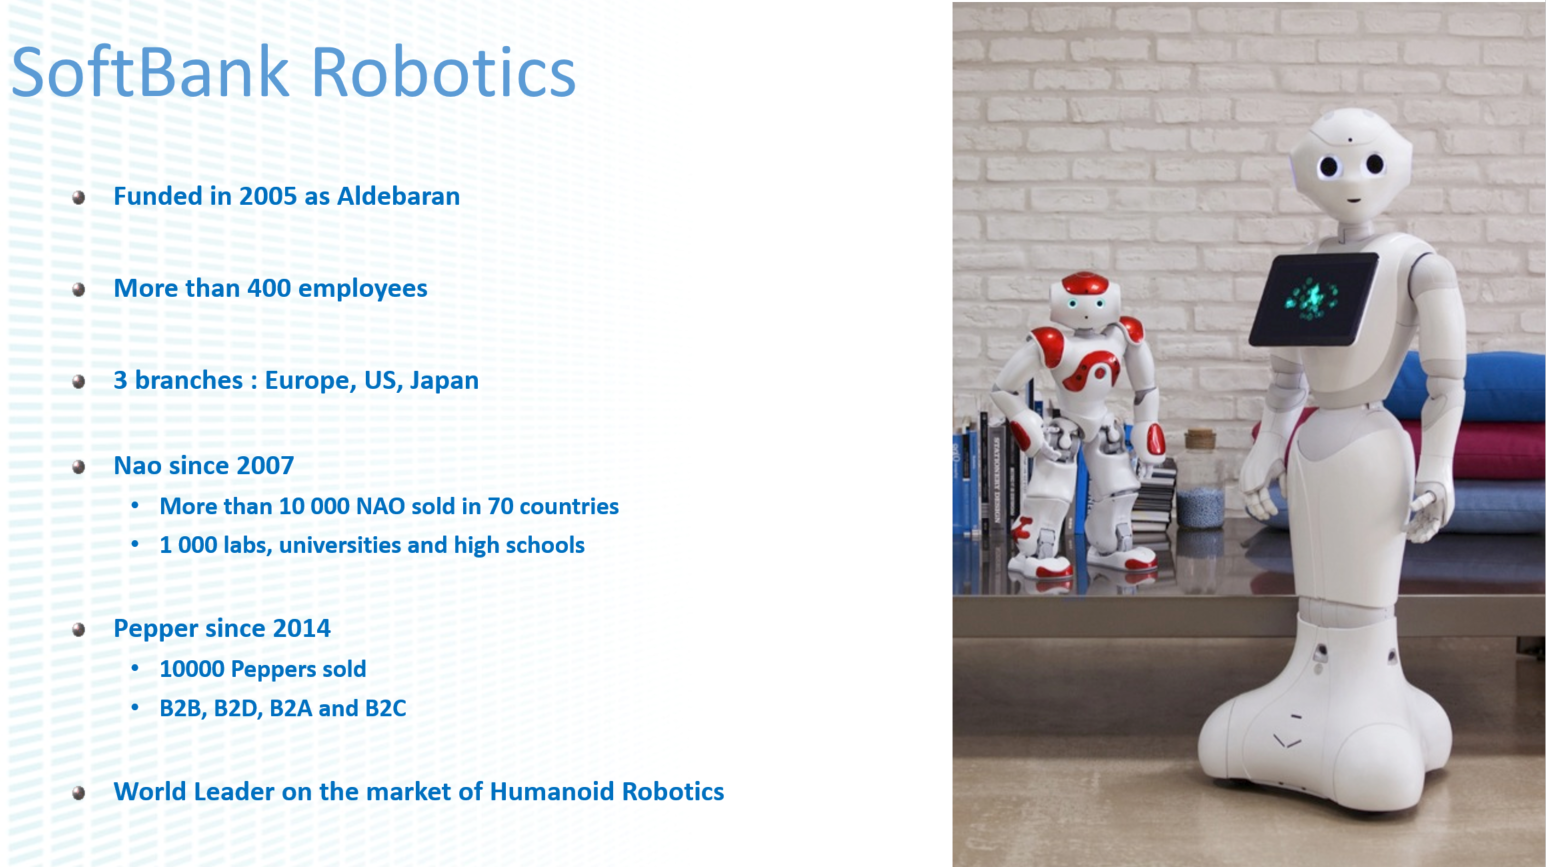
\includegraphics[width=\textwidth]{gelin1.png}
		\end{center}
	\end{frame}

	\begin{frame}
		\begin{center}
			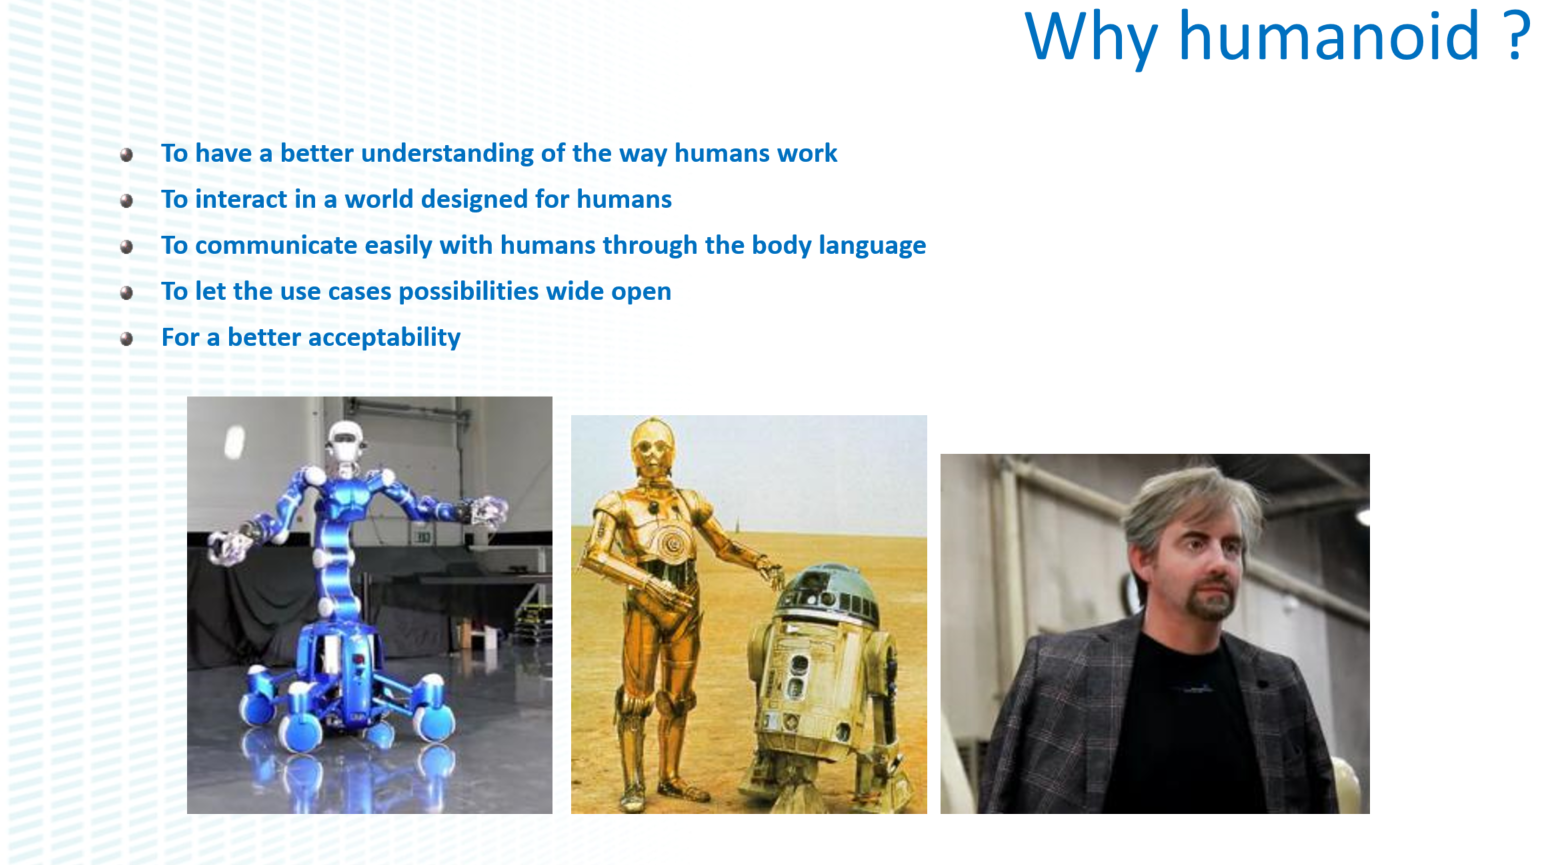
\includegraphics[width=\textwidth]{gelin2.png}
		\end{center}
	\end{frame}

	\begin{frame}
		\begin{center}
			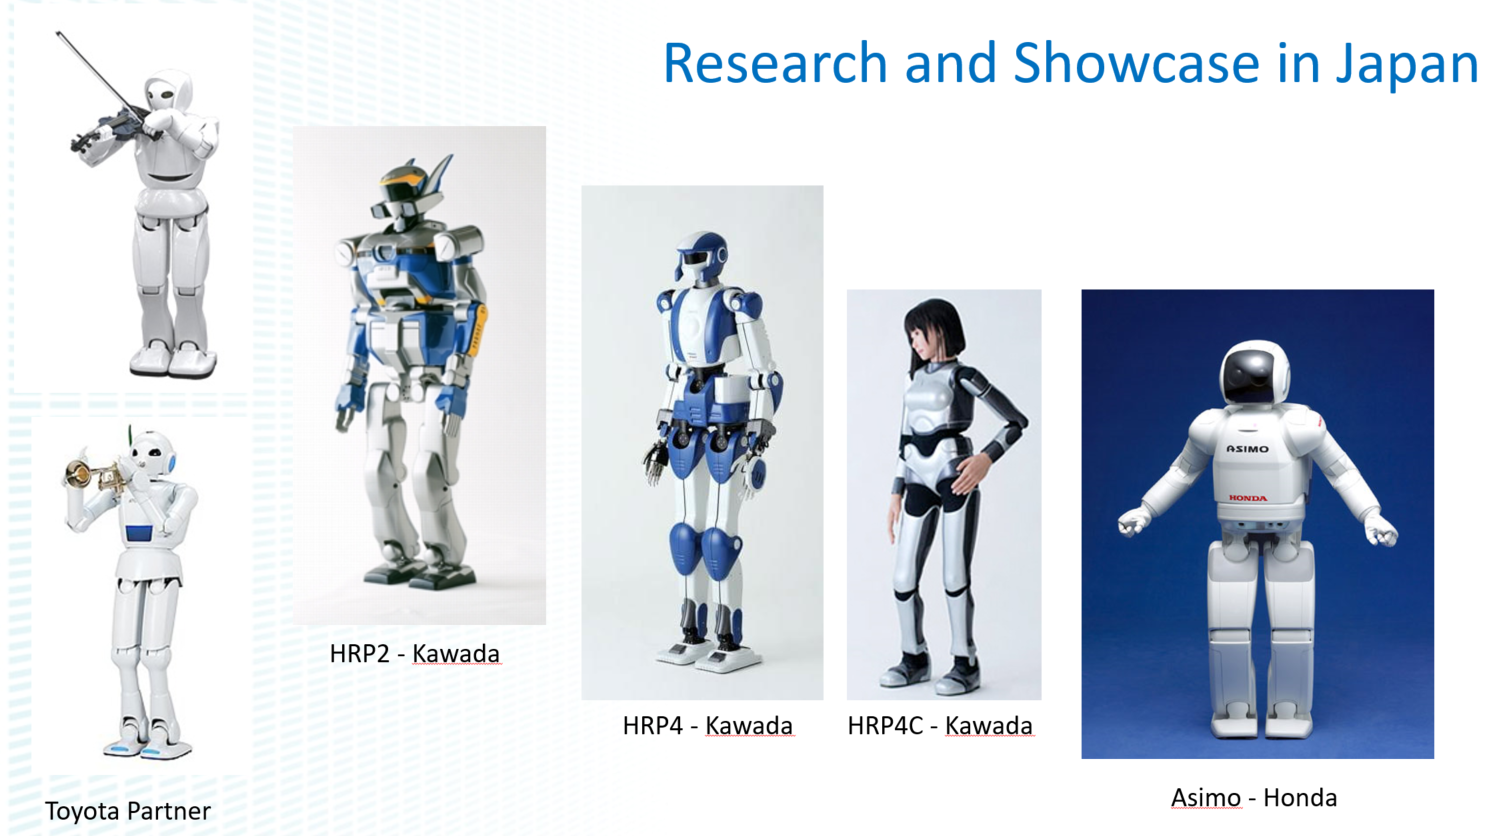
\includegraphics[width=\textwidth]{gelin3.png}
		\end{center}
	\end{frame}

	\begin{frame}
		\begin{center}
			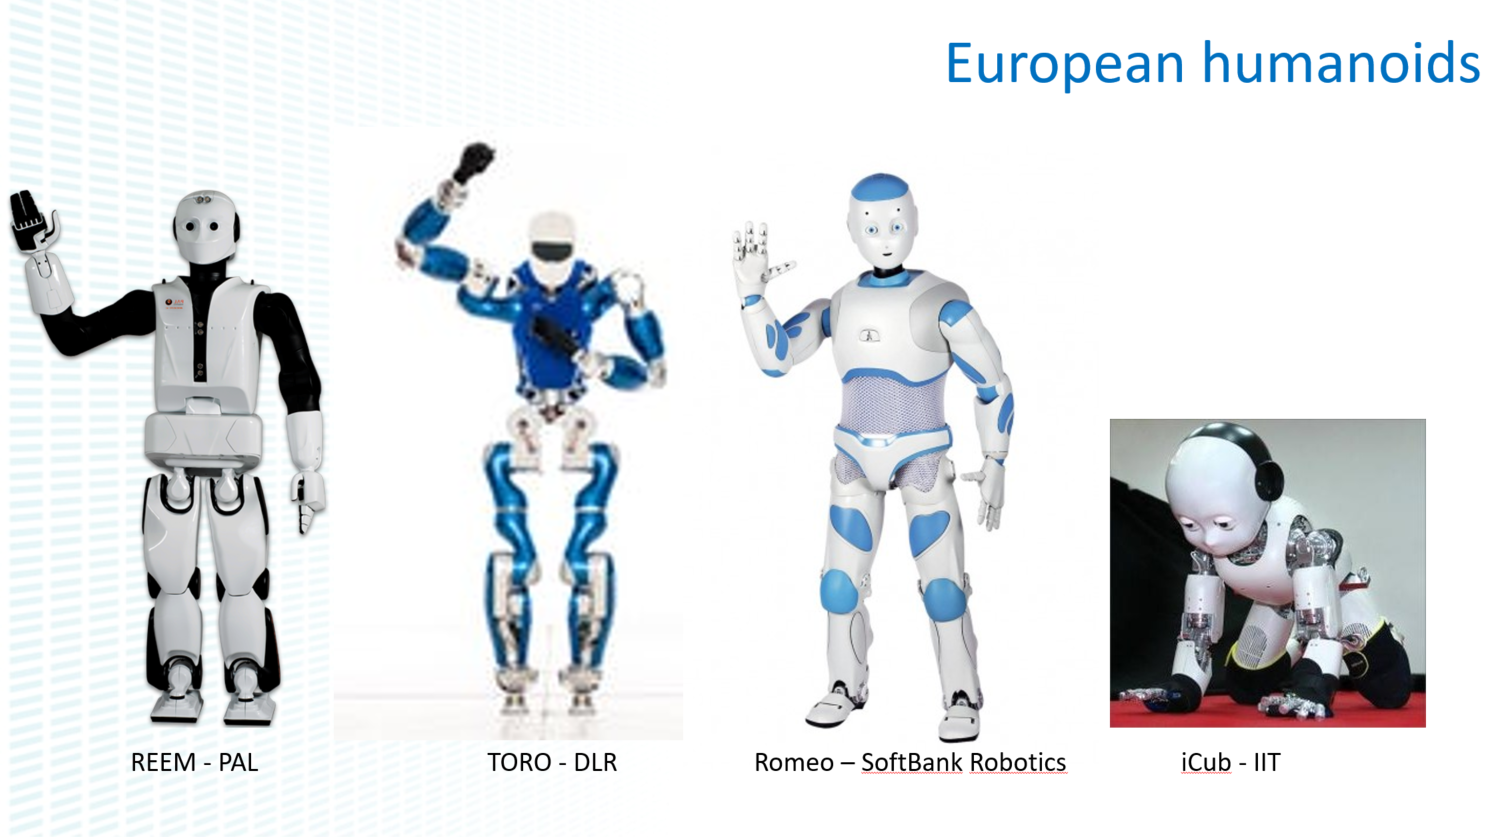
\includegraphics[width=\textwidth]{gelin4.png}
		\end{center}
	\end{frame}

	\begin{frame}
		\begin{center}
			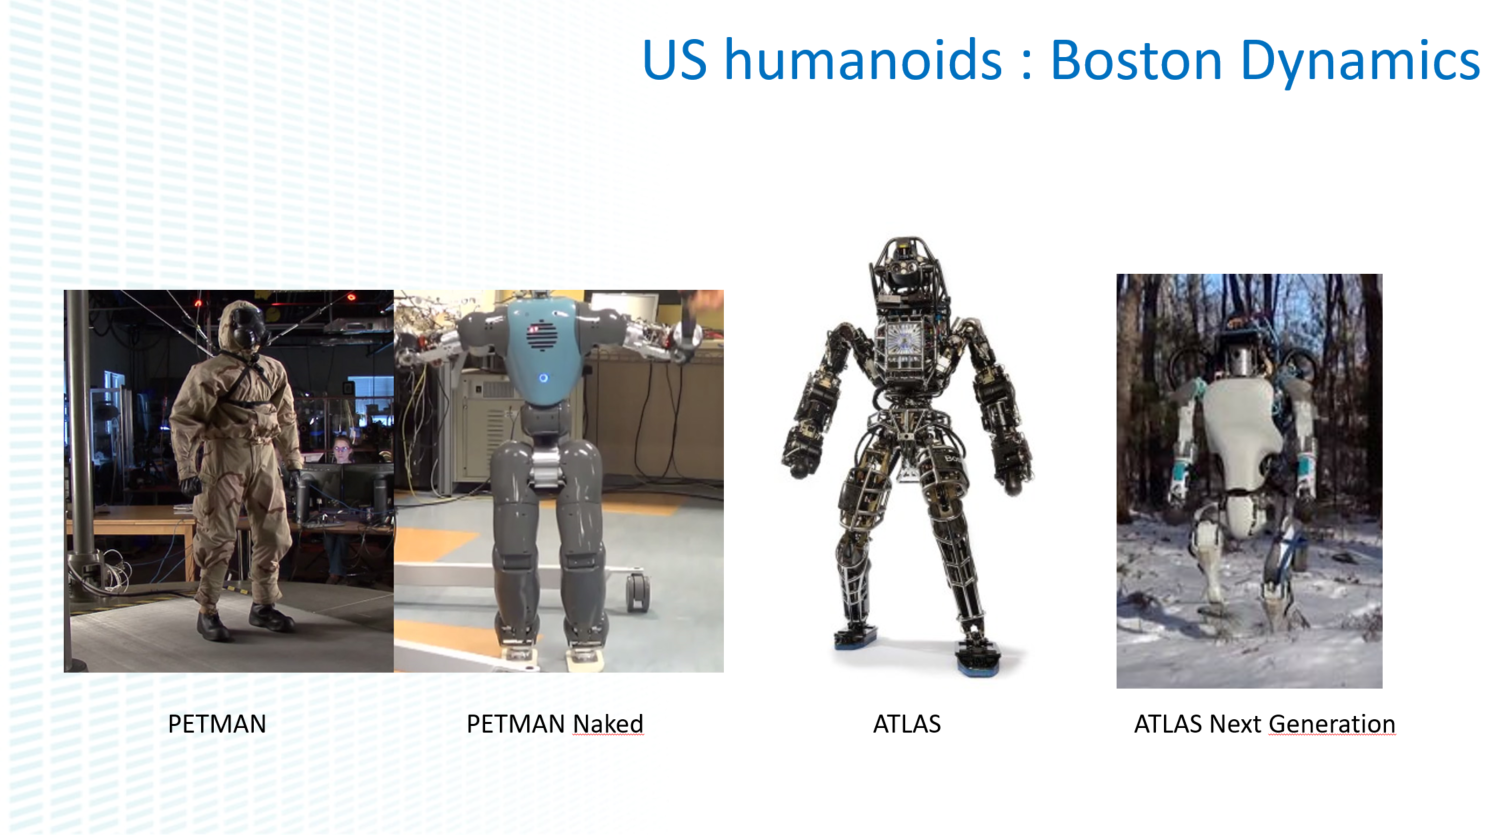
\includegraphics[width=\textwidth]{gelin5.png}
		\end{center}
	\end{frame}

	\begin{frame}
		\begin{center}
			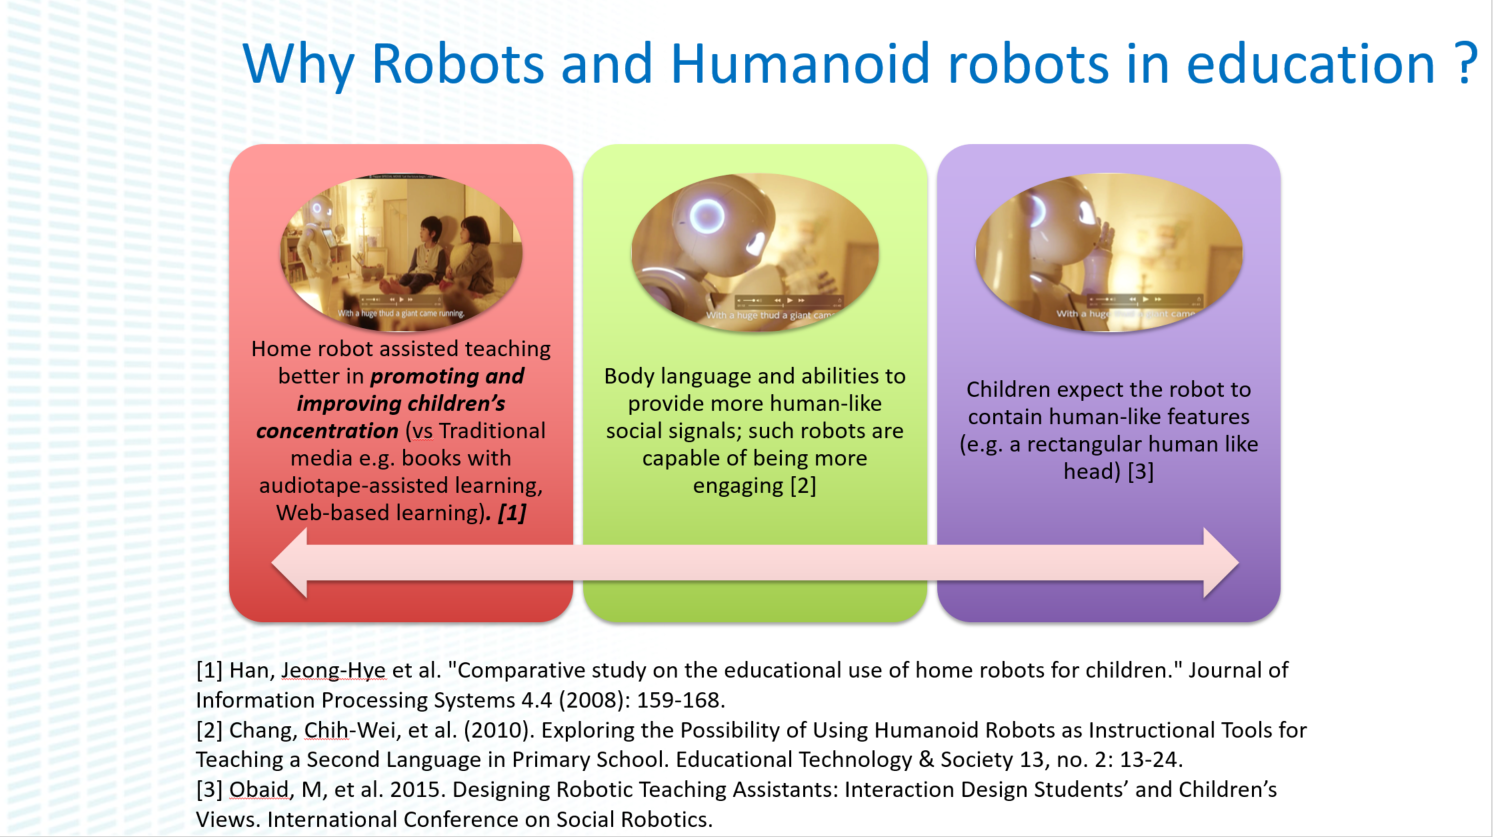
\includegraphics[width=\textwidth]{gelin6.png}
		\end{center}
	\end{frame}

	\begin{frame}
		\begin{center}
			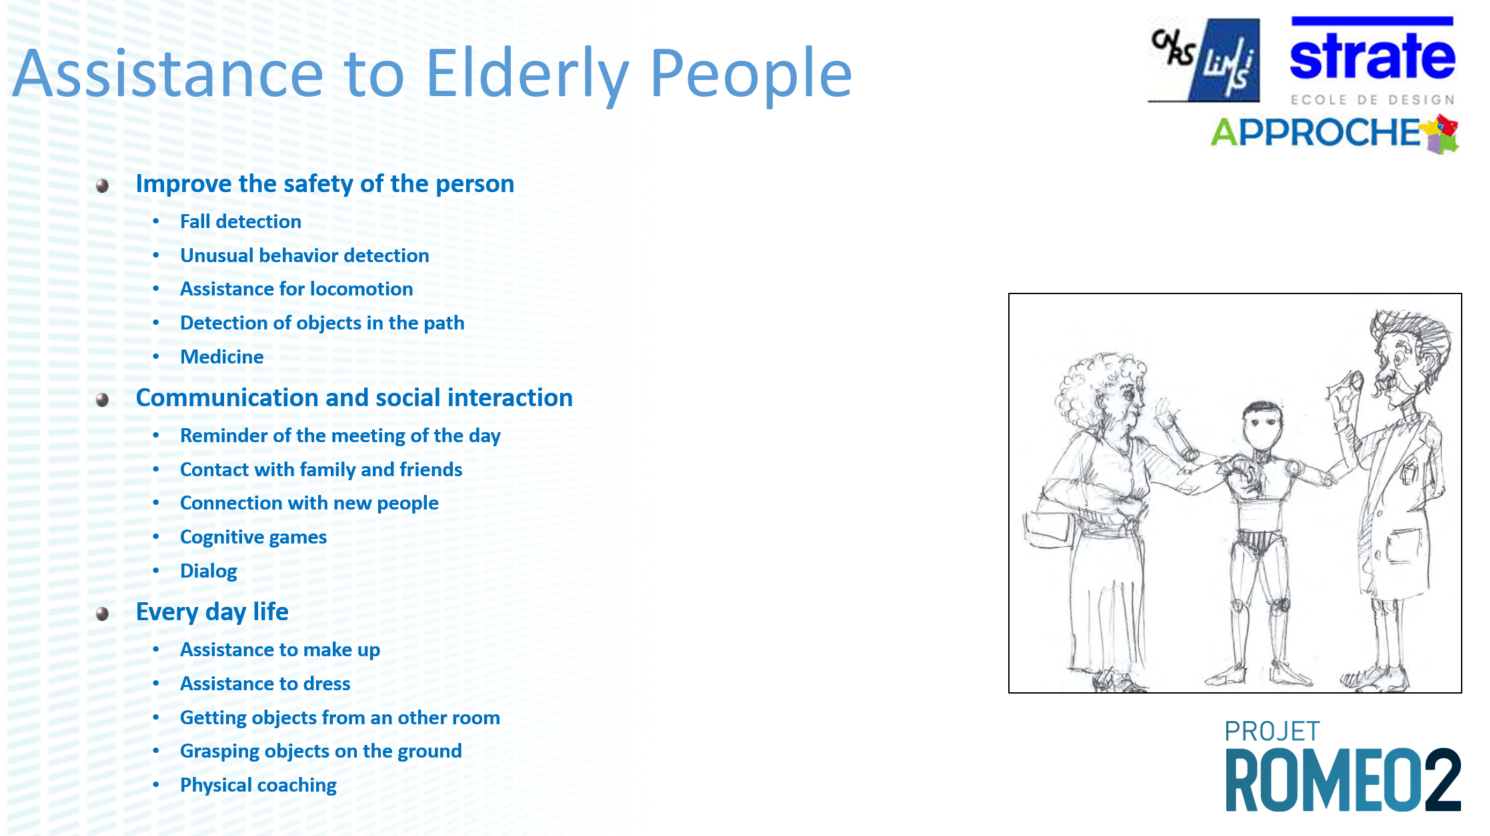
\includegraphics[width=\textwidth]{gelin7.png}
		\end{center}
	\end{frame}

	\begin{frame}
		\begin{center}
			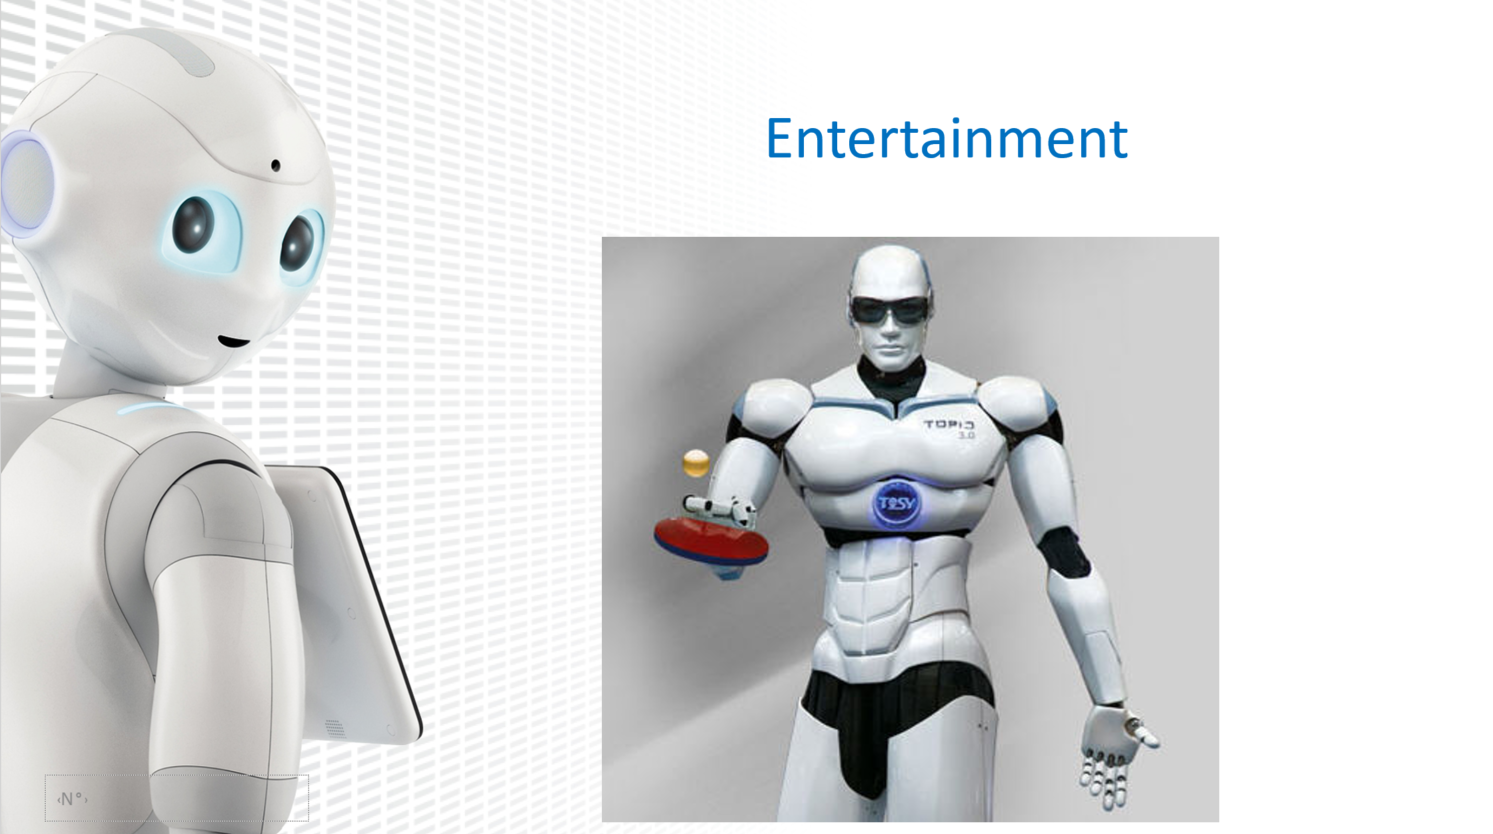
\includegraphics[width=\textwidth]{gelin8.png}
		\end{center}
	\end{frame}

	\begin{frame}
		\begin{center}
			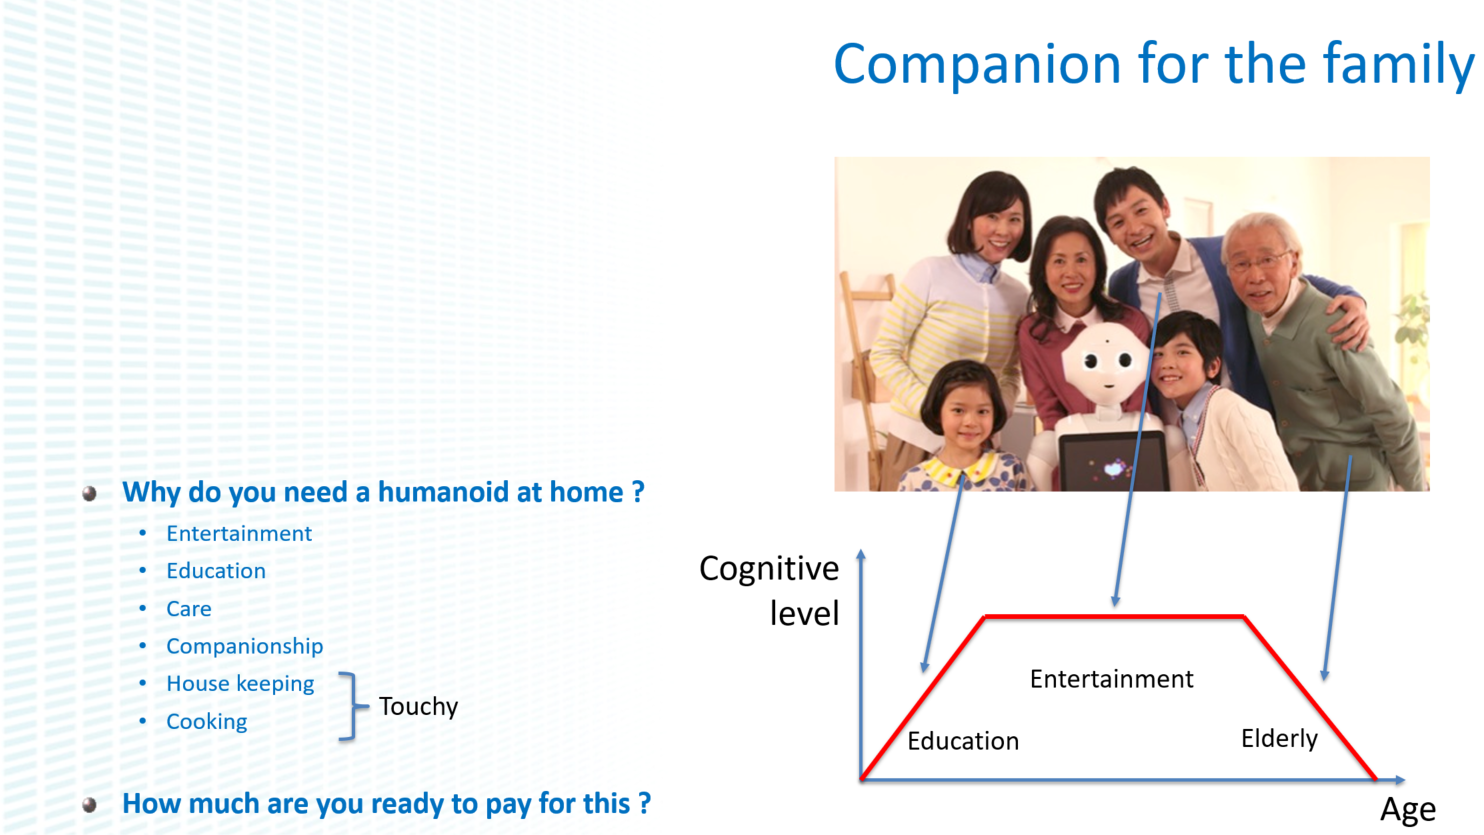
\includegraphics[width=\textwidth]{gelin9.png}
		\end{center}
	\end{frame}

	\begin{frame}
		\begin{center}
			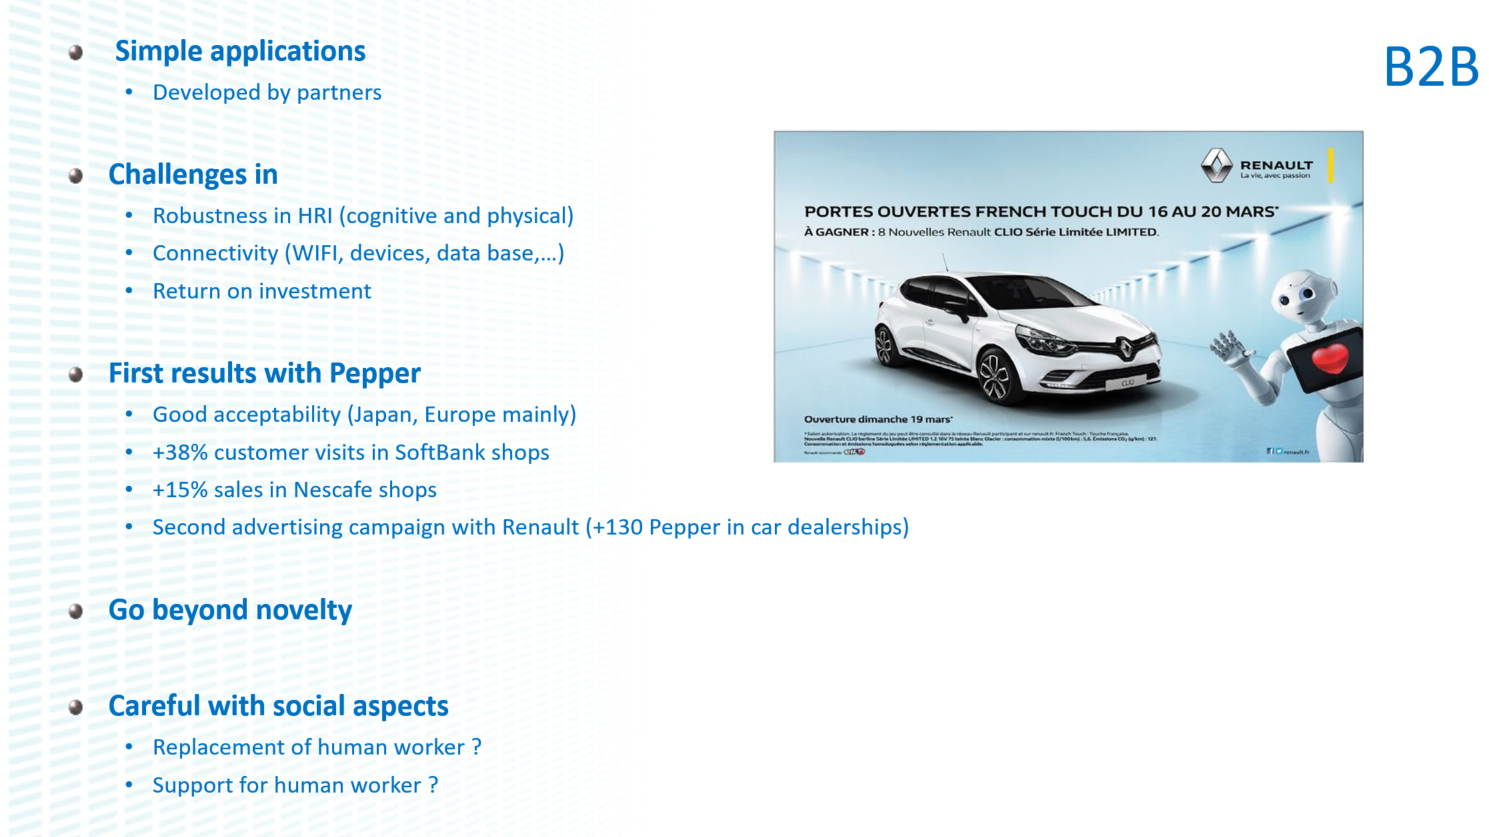
\includegraphics[width=\textwidth]{gelin10.png}
		\end{center}
	\end{frame}

	\begin{frame}
		\begin{center}
			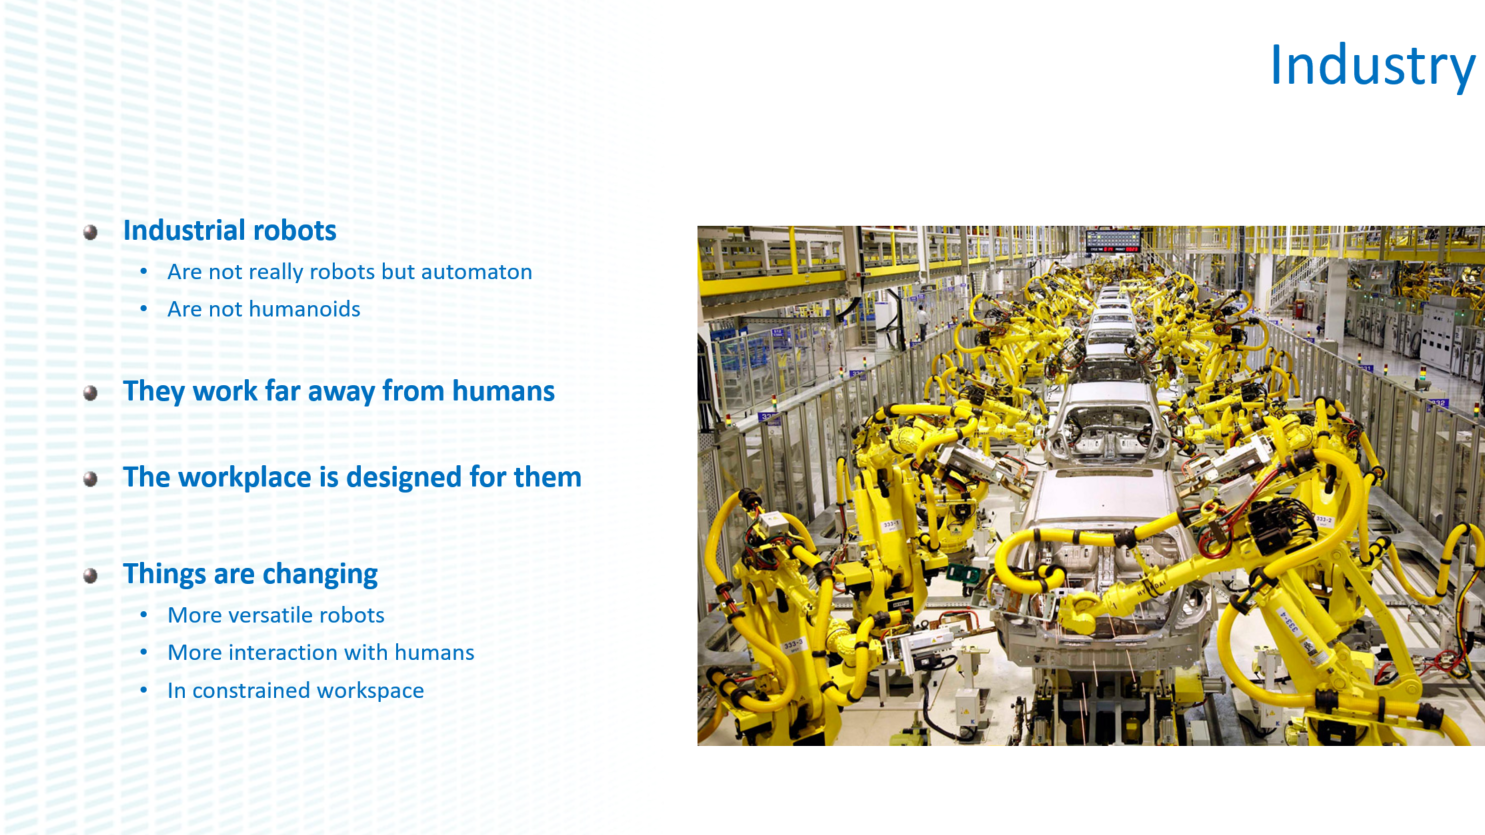
\includegraphics[width=\textwidth]{gelin11.png}
		\end{center}
	\end{frame}

	\begin{frame}
		\begin{center}
			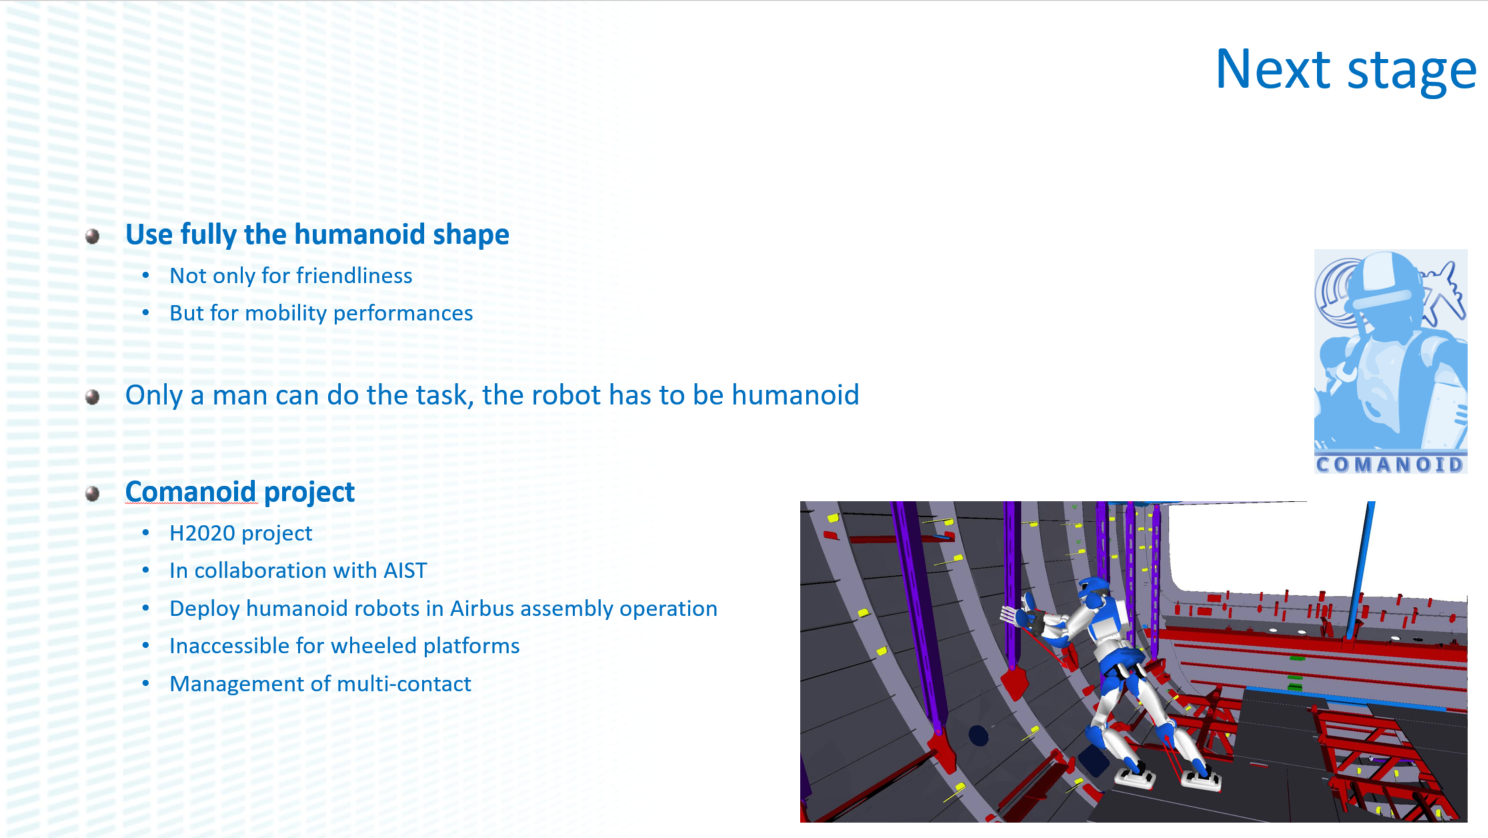
\includegraphics[width=\textwidth]{gelin12.png}
		\end{center}
	\end{frame}

	\begin{frame}
		\begin{center}
			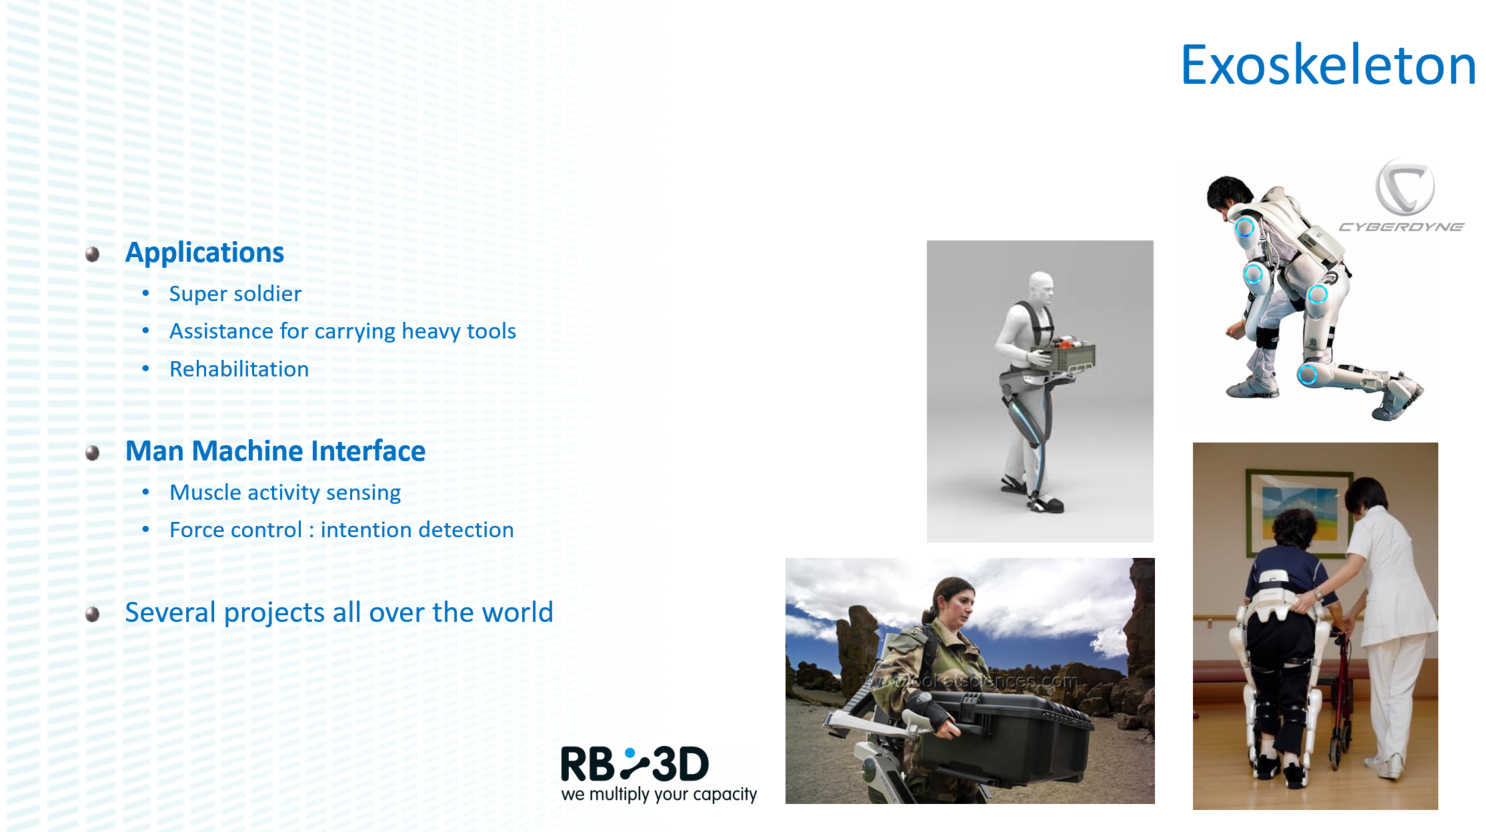
\includegraphics[width=\textwidth]{gelin13.png}
		\end{center}
	\end{frame}

	\begin{frame}
		\begin{center}
			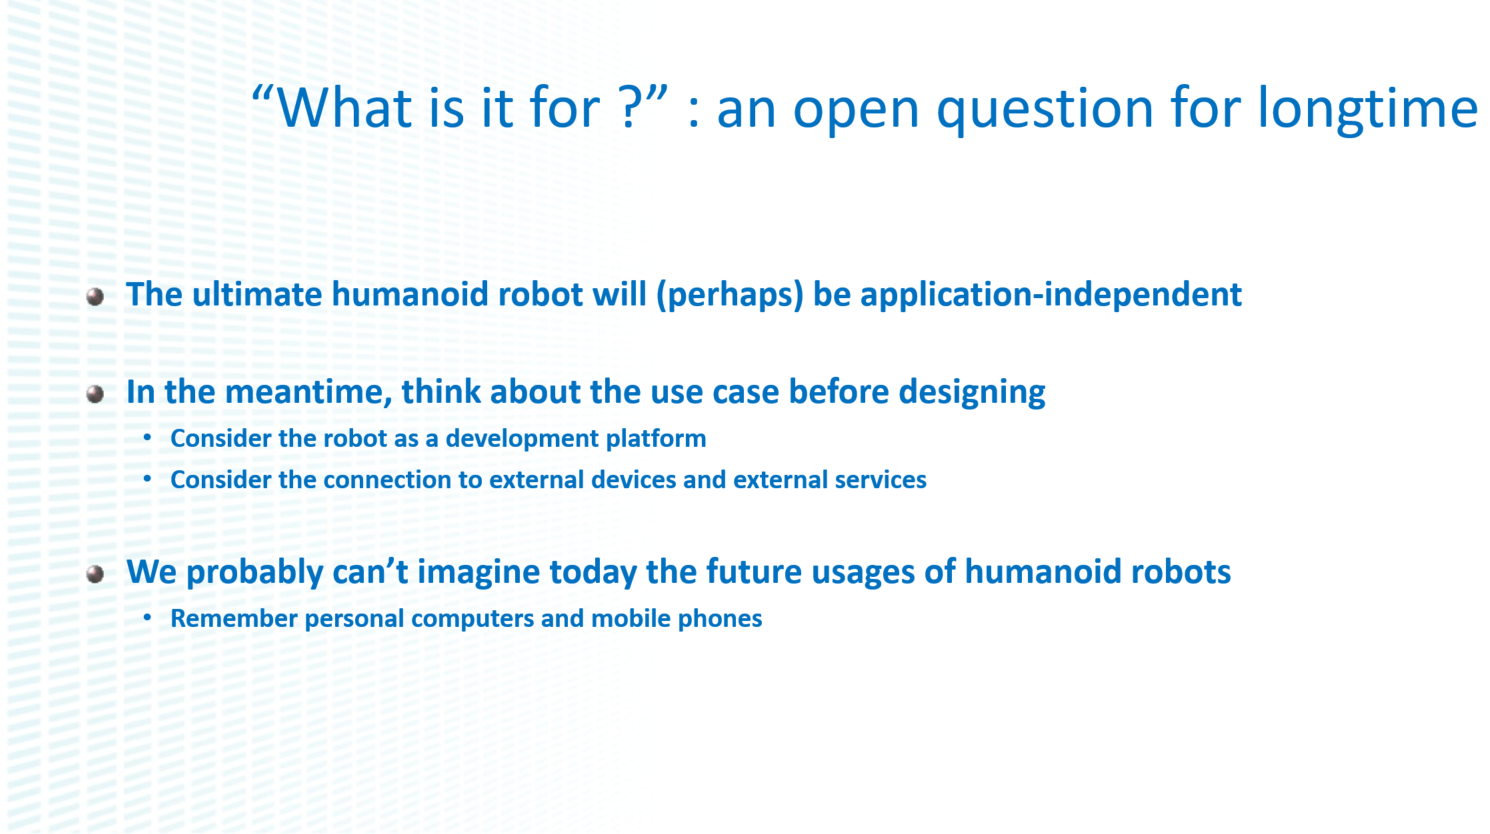
\includegraphics[width=\textwidth]{gelin14.png}
		\end{center}
	\end{frame}

	\begin{frame}
		\frametitle{Сложности физического взаимодействия гуманоидных роботов}
		\begin{itemize}
			\item Избежание самостолкновений
			\item Проблема приоритетов параллельно исполняемых задач
			\item Динамический выбор регуляторов для движения
			\item Избежание препятствий
			\item Навигация
			\item SLAM
			\item Захват объектов
			\item Управление силой, обратная связь
		\end{itemize}
	\end{frame}

	\begin{frame}
		\begin{center}
			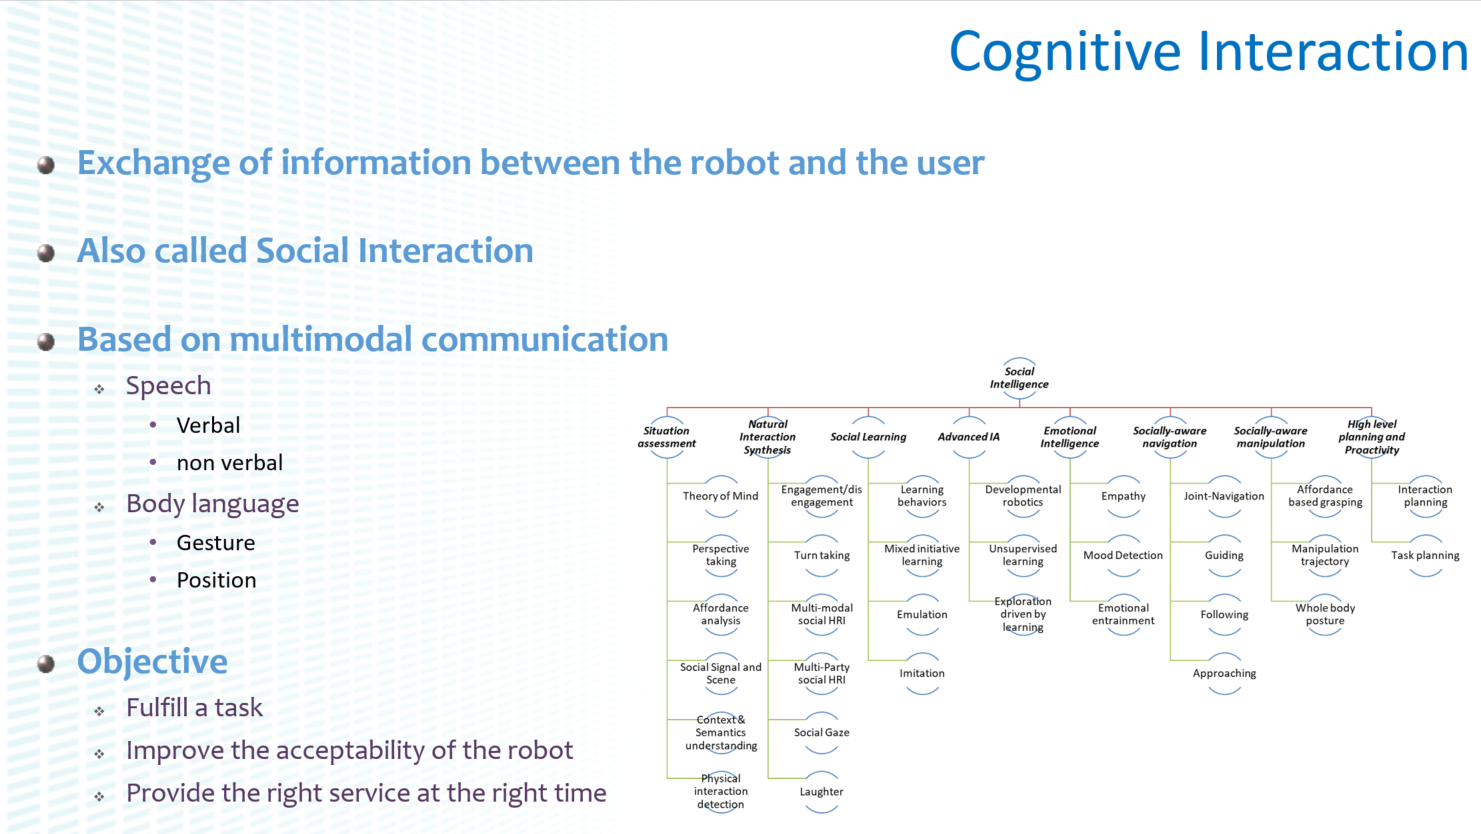
\includegraphics[width=\textwidth]{gelin15.png}
		\end{center}
	\end{frame}

	\begin{frame}
		\begin{center}
			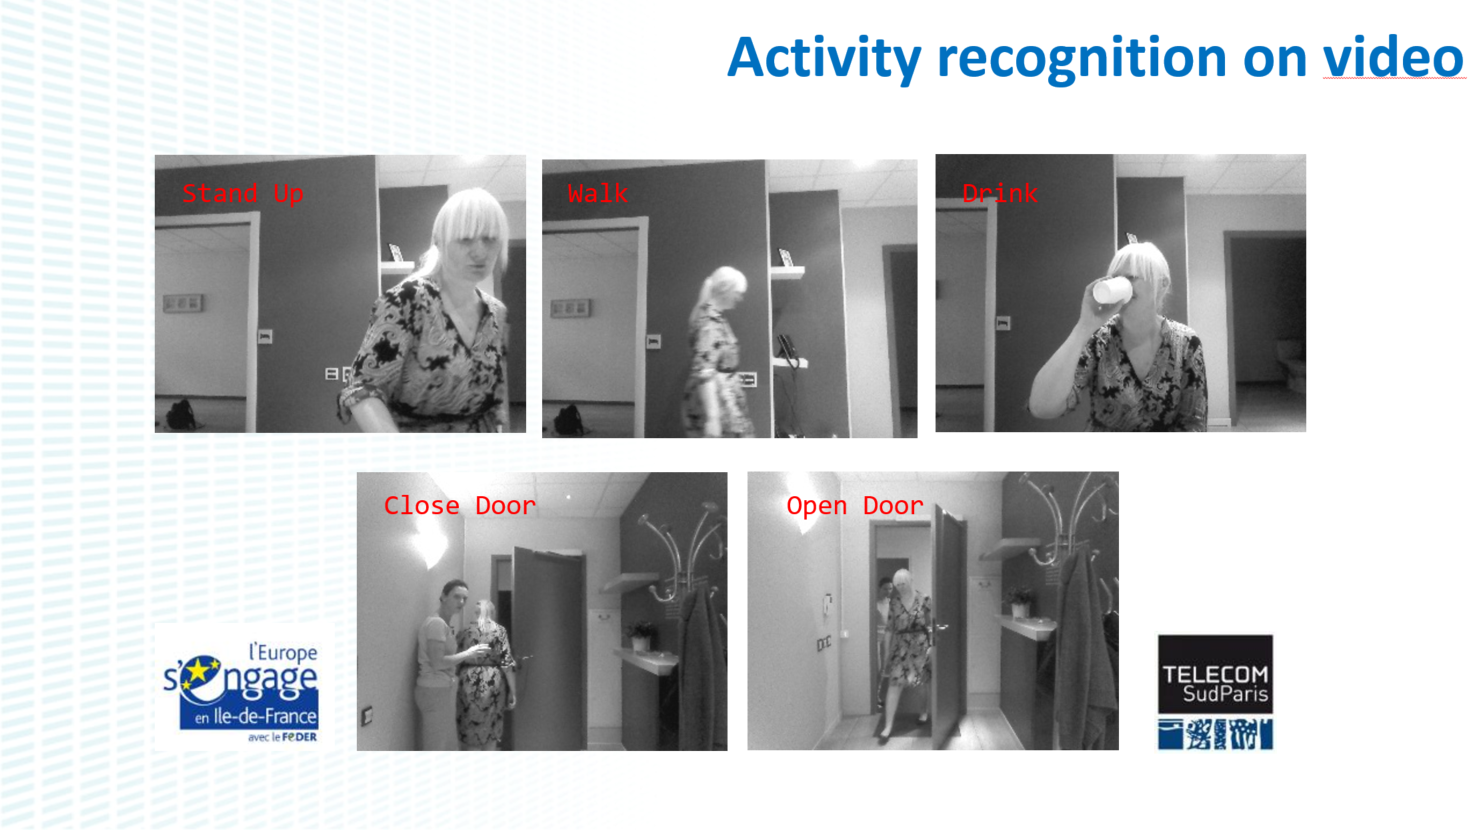
\includegraphics[width=\textwidth]{gelin16.png}
		\end{center}
	\end{frame}

	\begin{frame}
		\begin{center}
			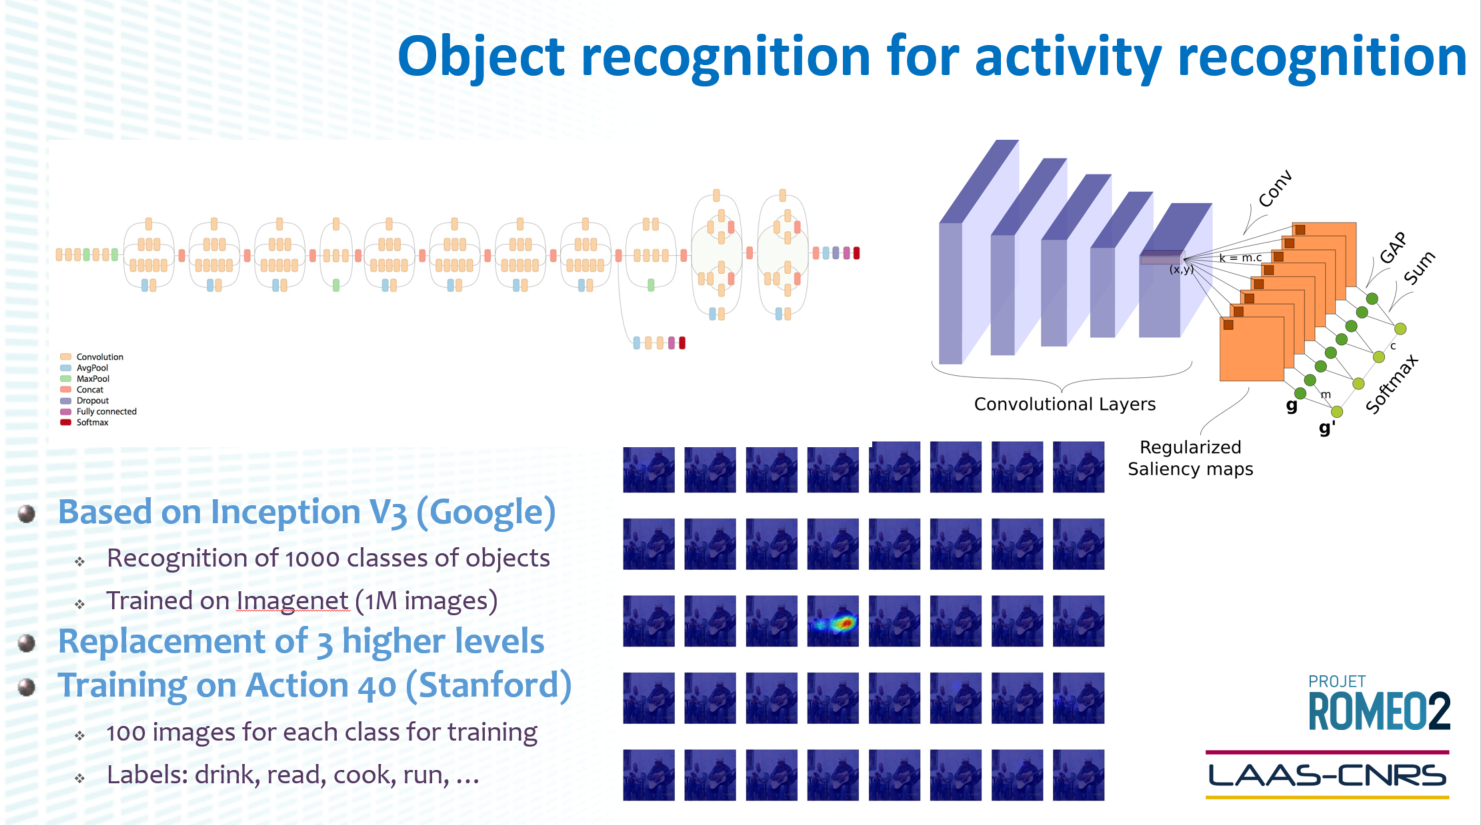
\includegraphics[width=\textwidth]{gelin17.png}
		\end{center}
	\end{frame}

	\begin{frame}
		\begin{center}
			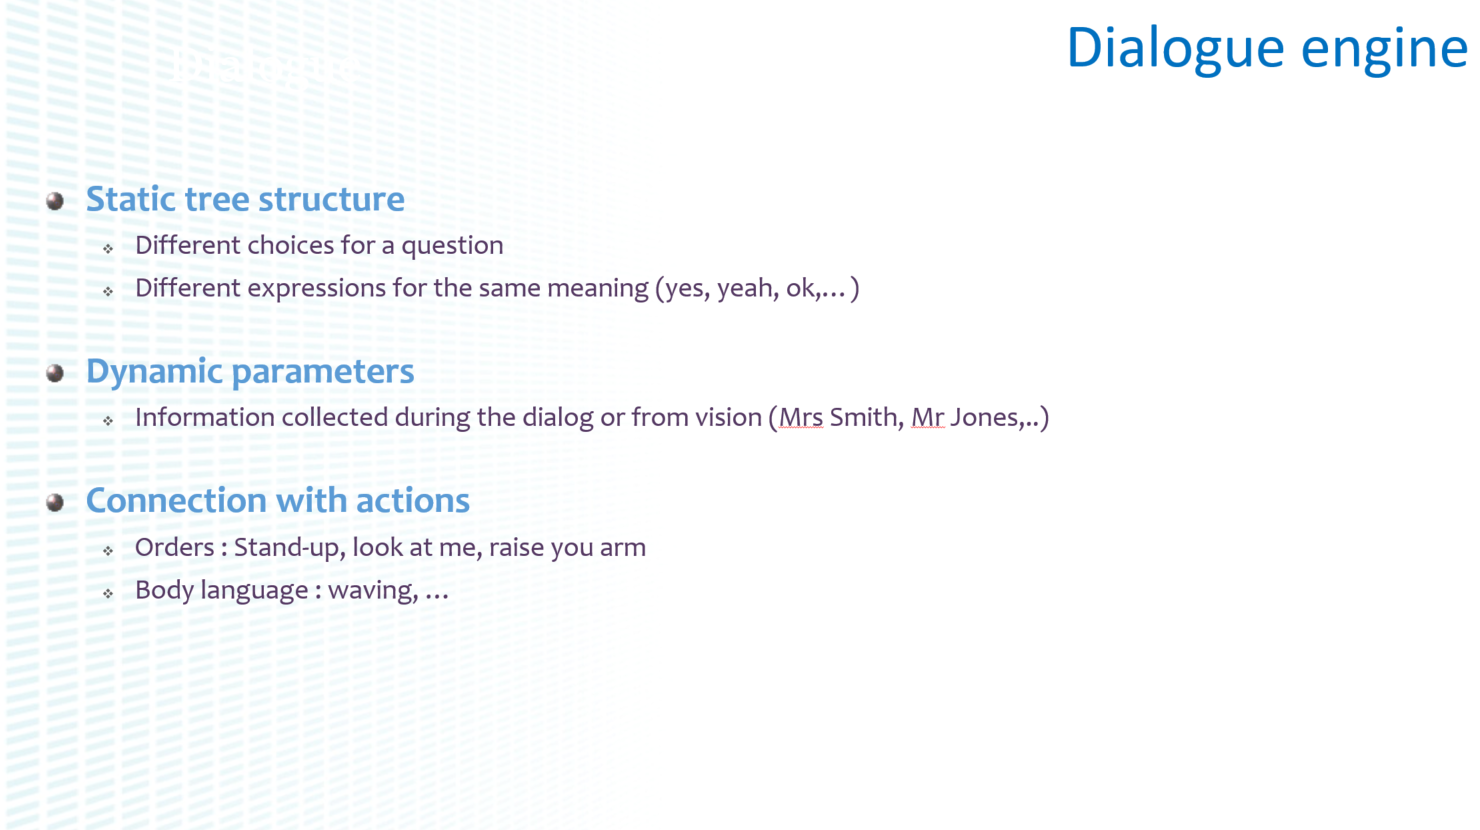
\includegraphics[width=\textwidth]{gelin18.png}
		\end{center}
	\end{frame}

	\begin{frame}
		\begin{center}
			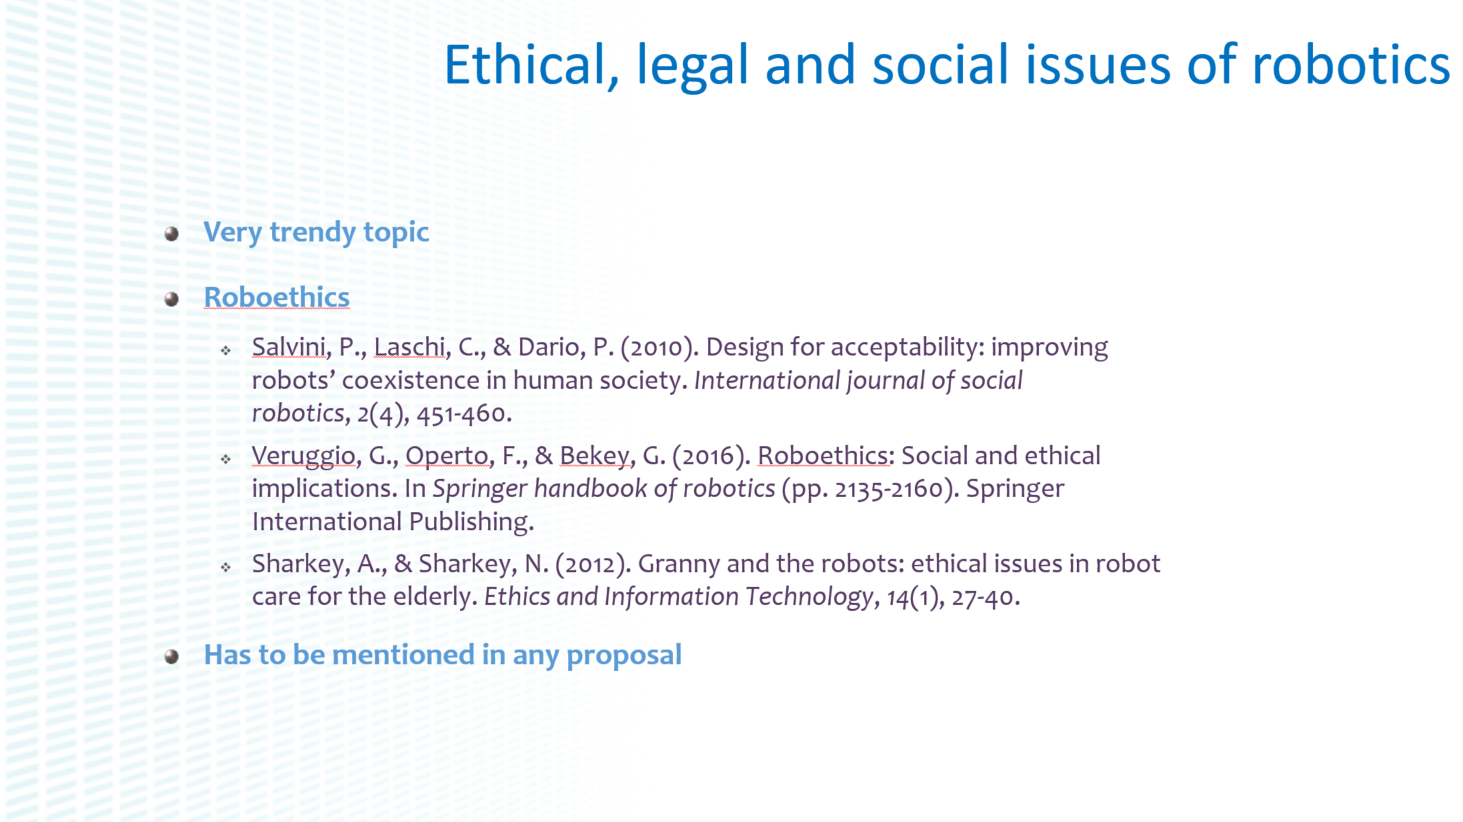
\includegraphics[width=\textwidth]{gelin19.png}
		\end{center}
	\end{frame}

	\begin{frame}
		\begin{center}
			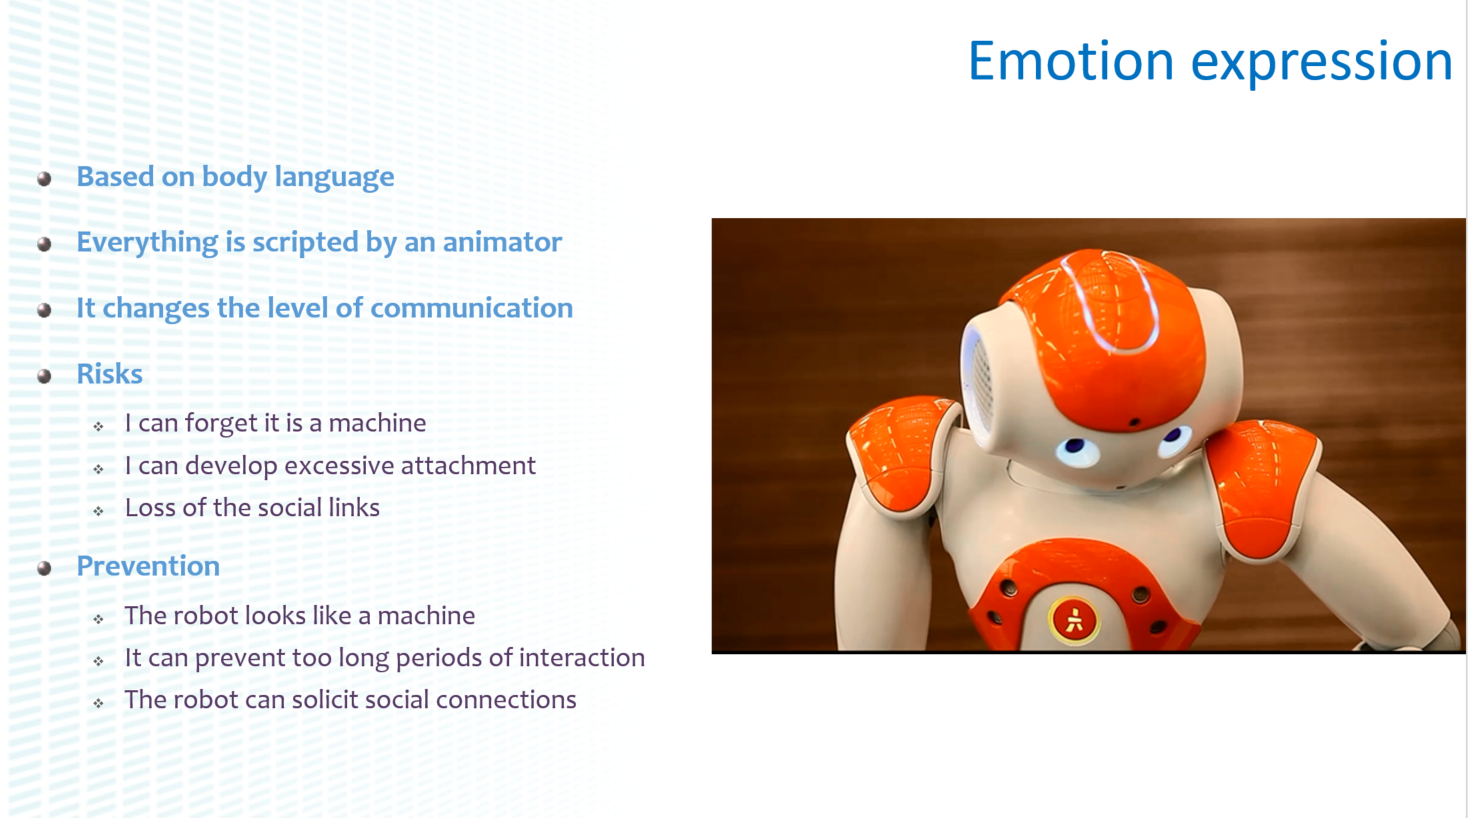
\includegraphics[width=\textwidth]{gelin20.png}
		\end{center}
	\end{frame}

	\begin{frame}
		\begin{center}
			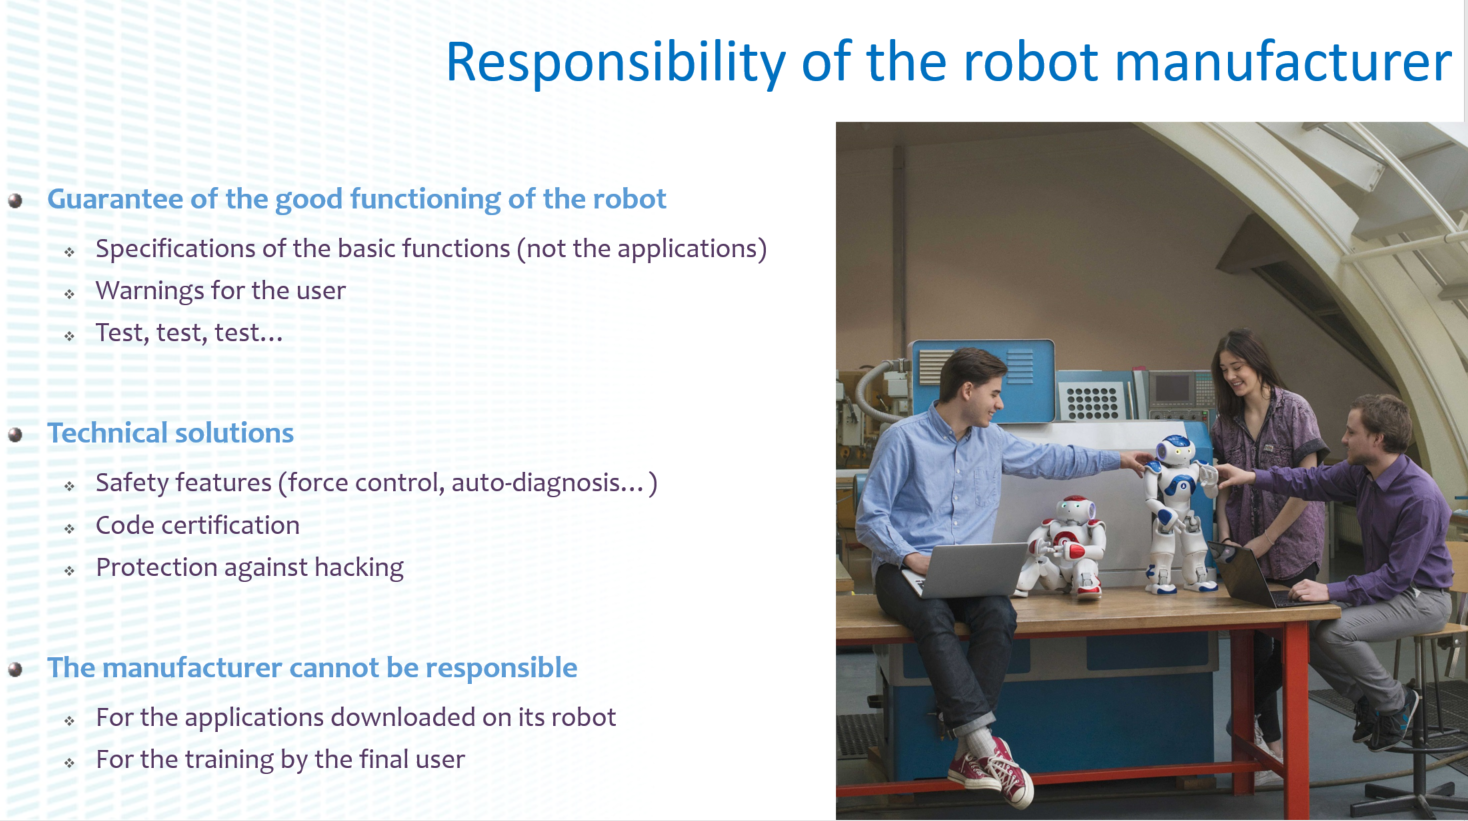
\includegraphics[width=\textwidth]{gelin21.png}
		\end{center}
	\end{frame}

	\section{A. Kapoor}

	\begin{frame}
		\frametitle{Ashish Kapoor}
		\begin{itemize}
			\item Не выложил слайды!
			\item AirSim (\url{https://github.com/microsoft/airsim})
			\item Рассказывал в основном про обеспечение безопасности полёта квадрокоптера путём задания ограничений в виде вероятностных темпоральных логик
		\end{itemize}
		\begin{center}
			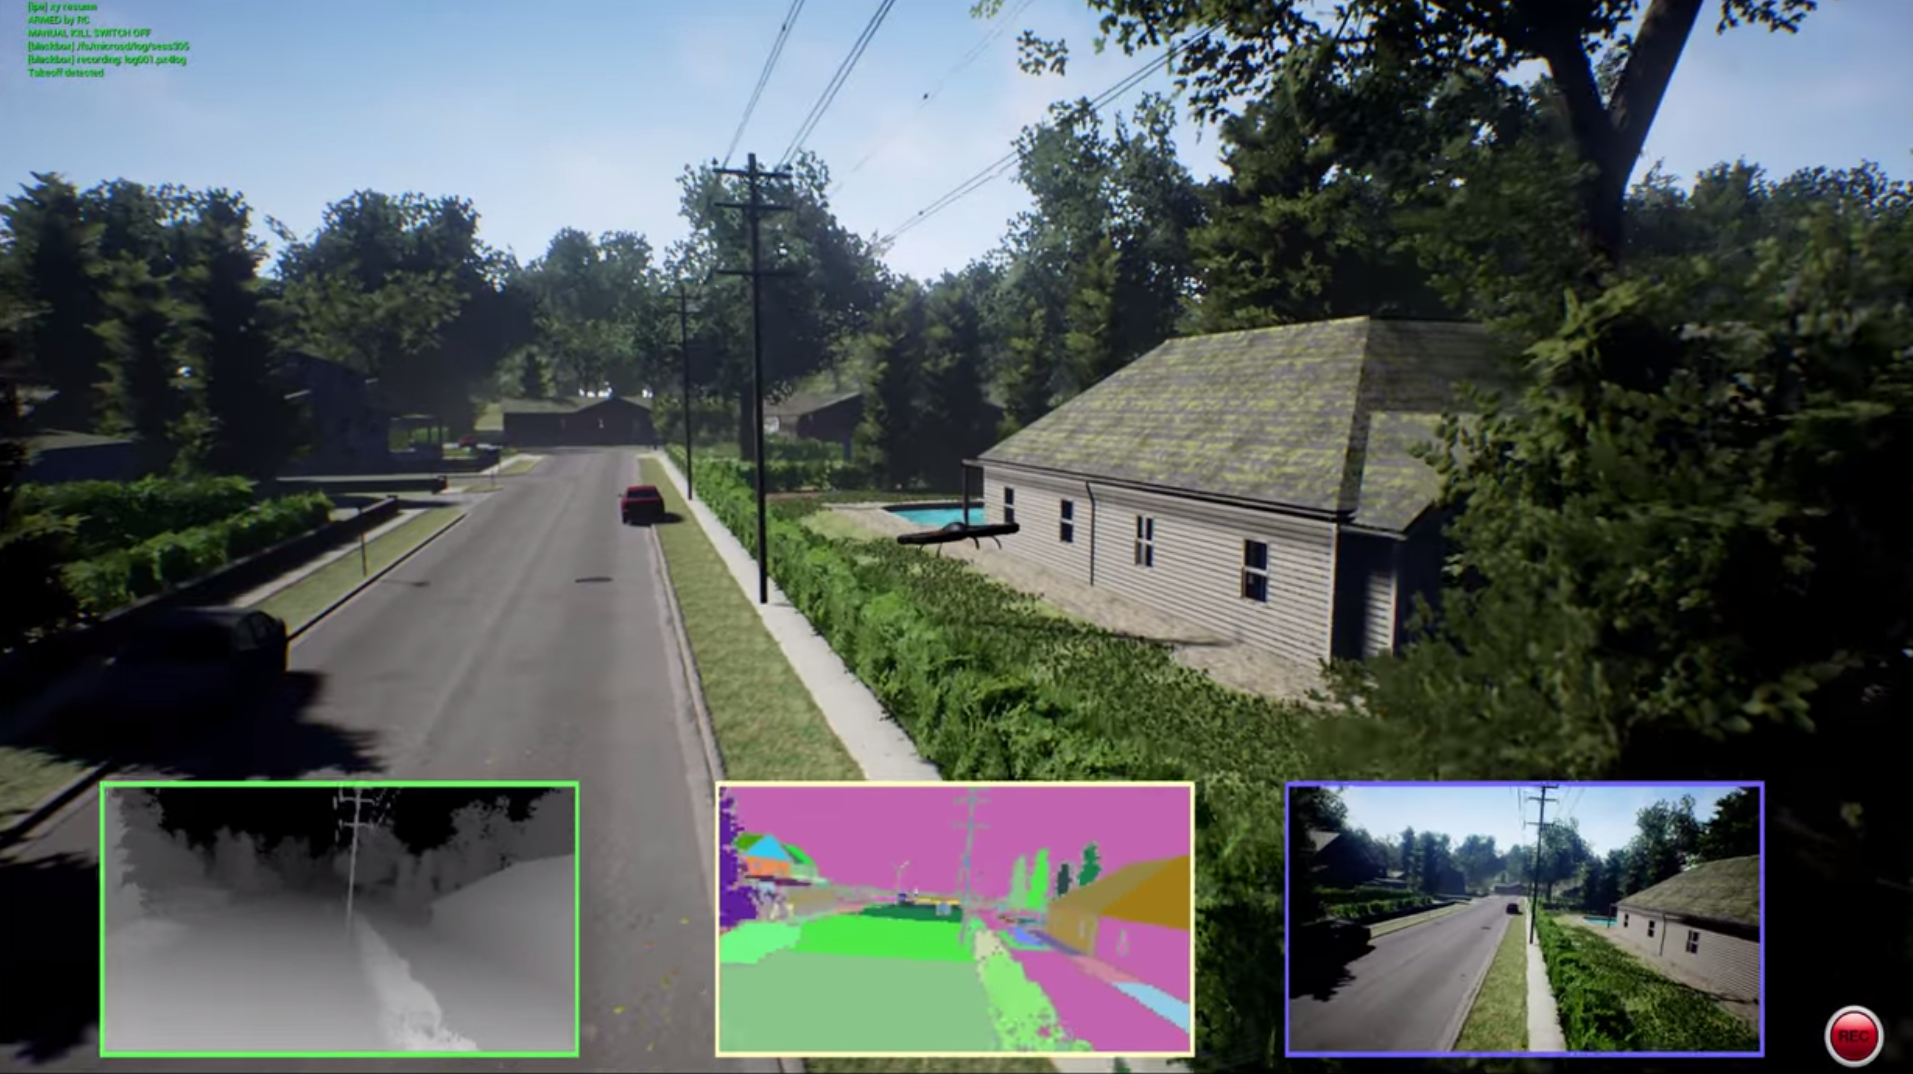
\includegraphics[width=0.5\textwidth]{airSim.png}
		\end{center}
	\end{frame}

	\section{N. Medvidovic}
	
	\begin{frame}
		\begin{center}
			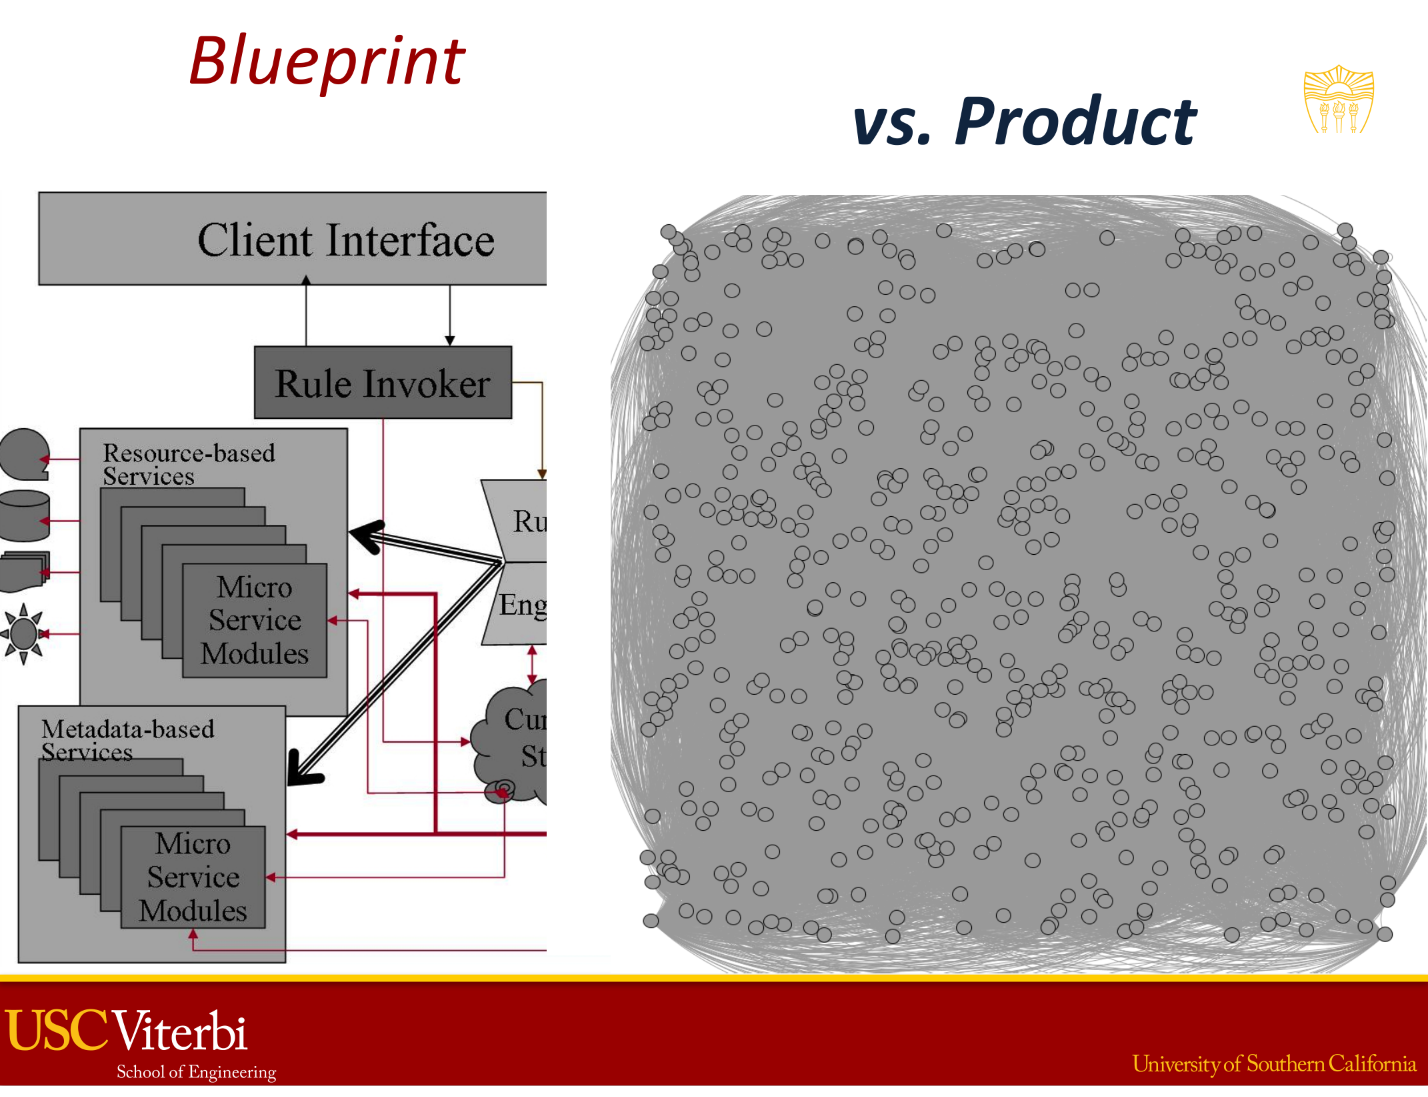
\includegraphics[width=0.9\textwidth]{medvidovic1.png}
		\end{center}
	\end{frame}

	\begin{frame}
		\begin{center}
			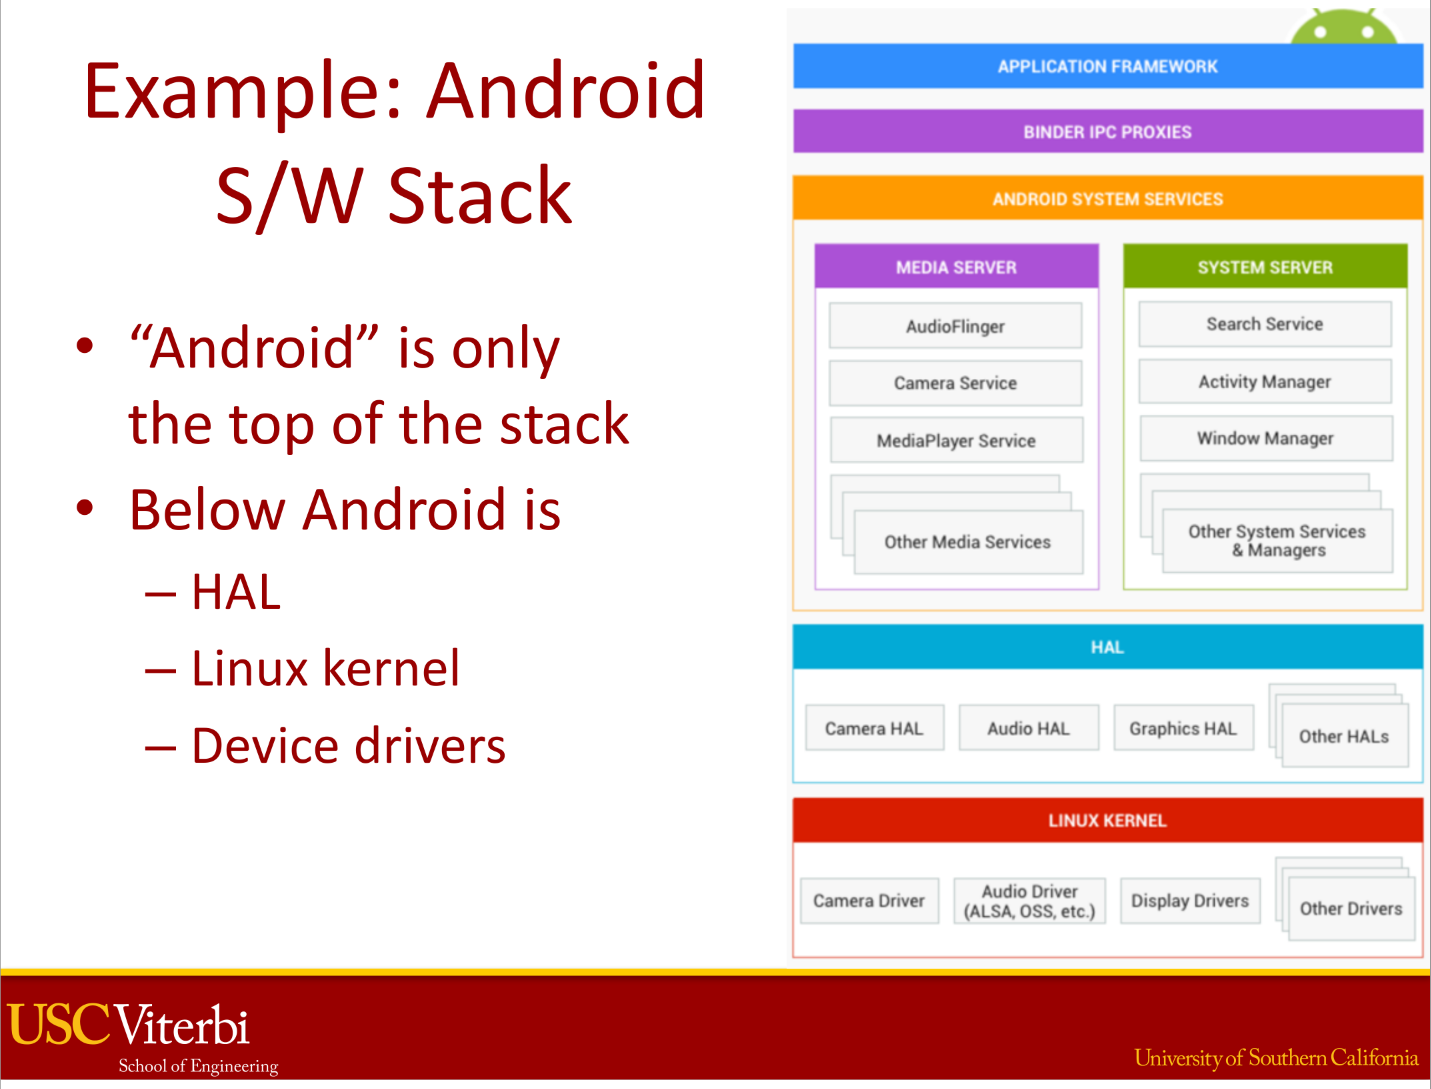
\includegraphics[width=0.9\textwidth]{medvidovic2.png}
		\end{center}
	\end{frame}

	\begin{frame}
		\begin{center}
			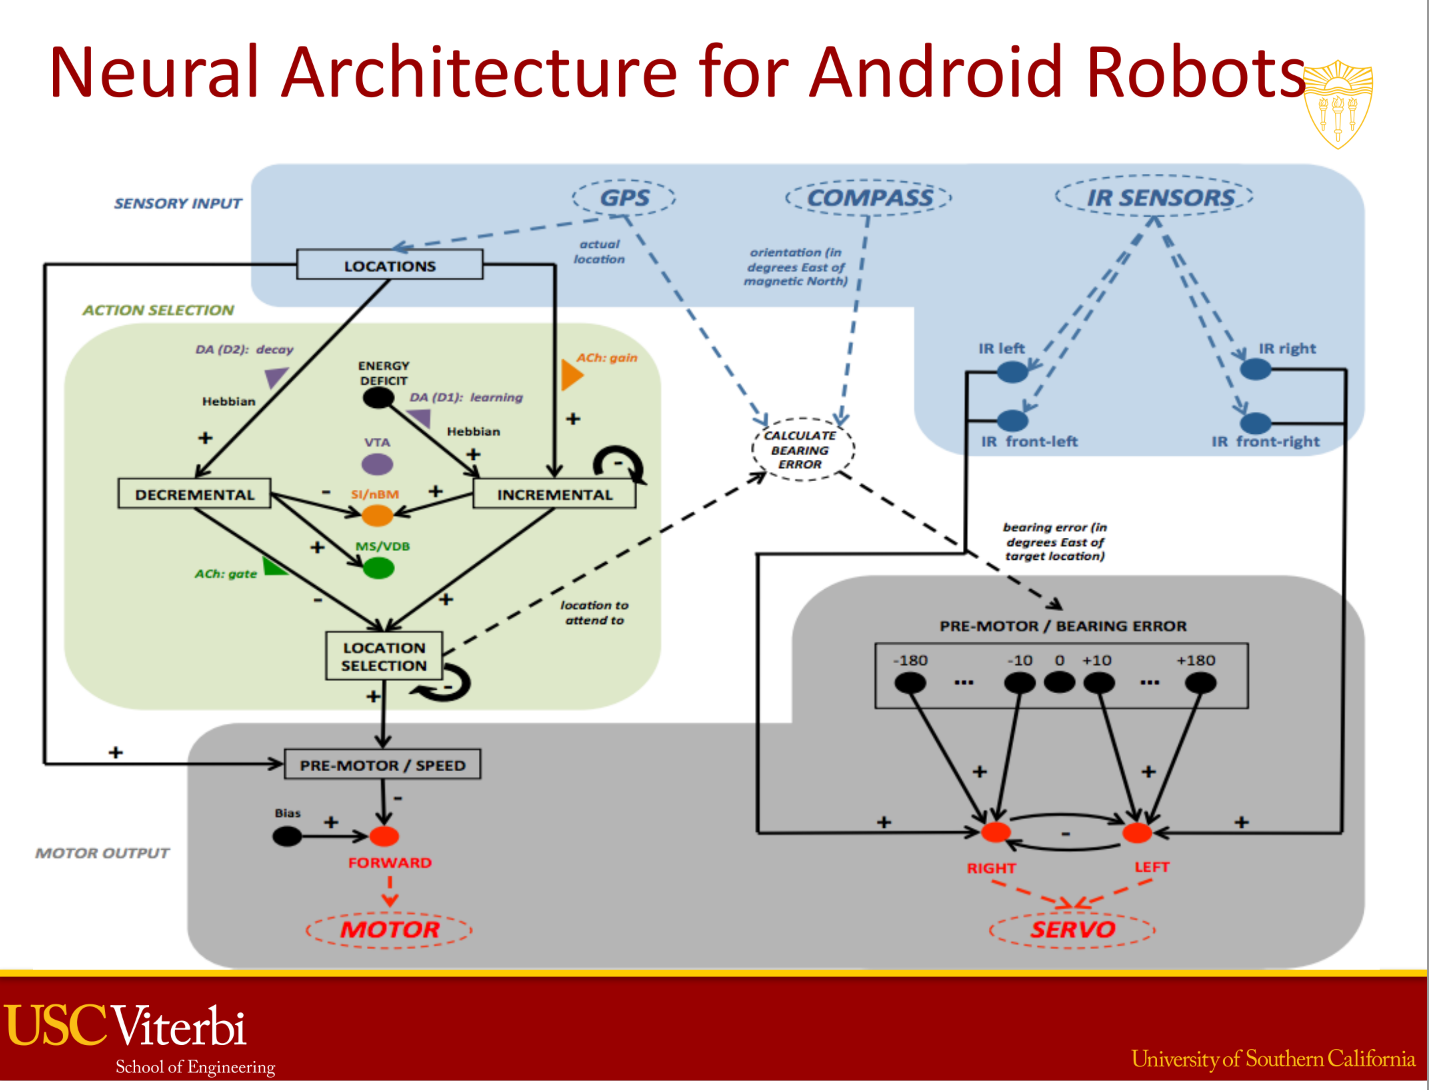
\includegraphics[width=0.9\textwidth]{medvidovic3.png}
		\end{center}
	\end{frame}

	\begin{frame}
		\begin{center}
			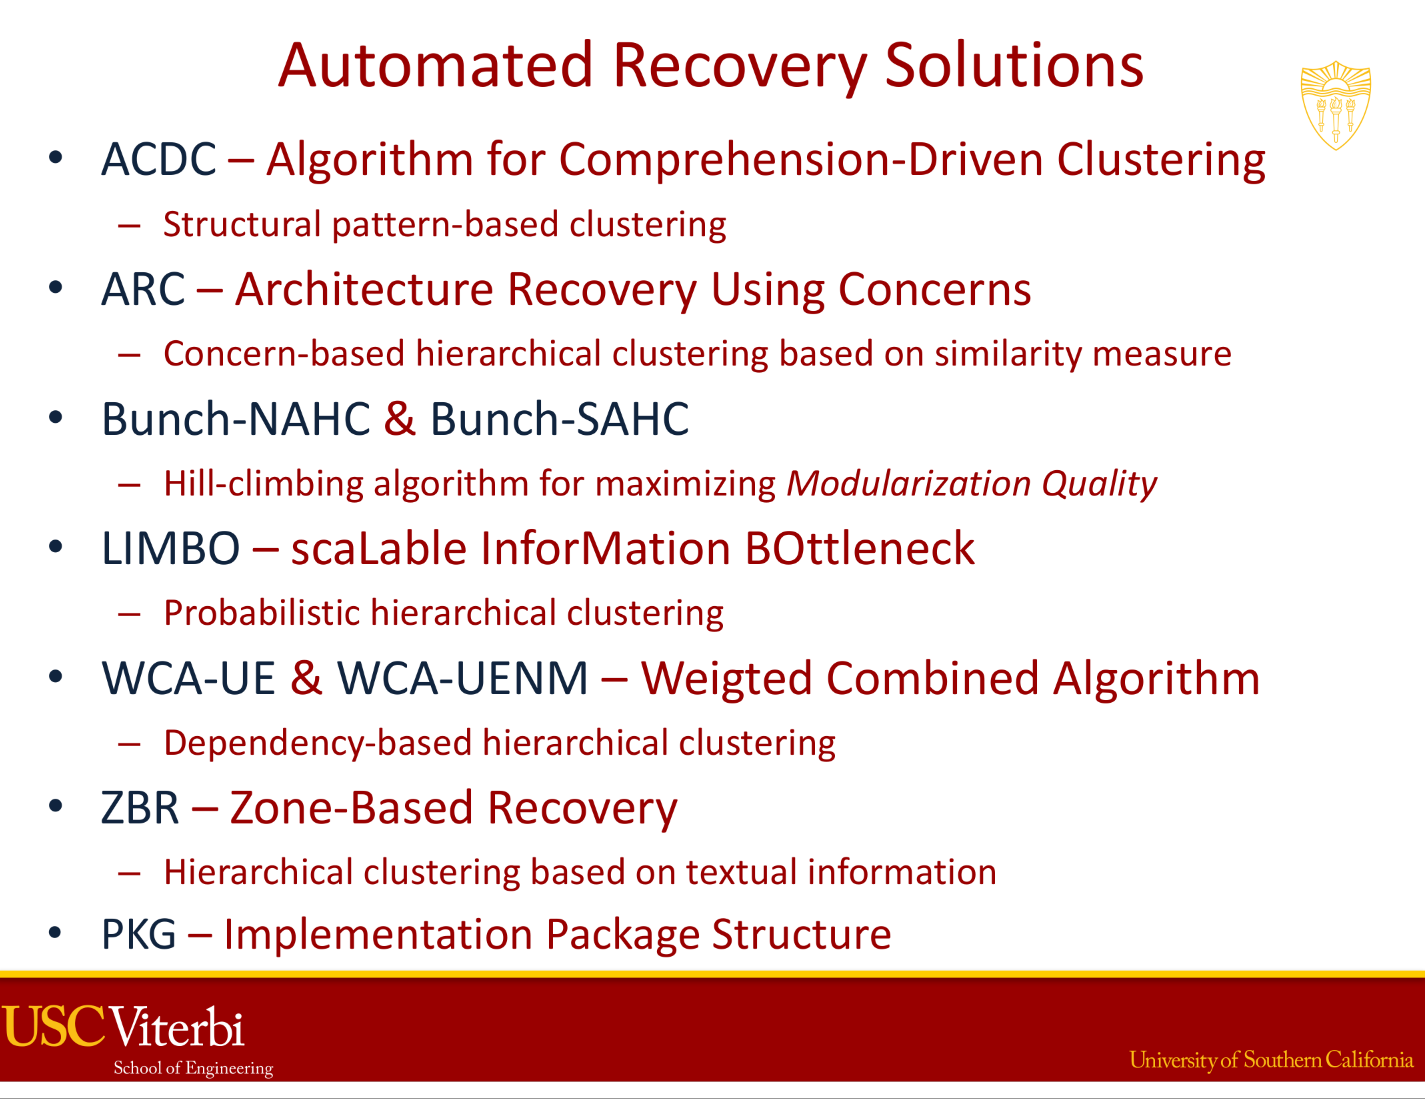
\includegraphics[width=0.9\textwidth]{medvidovic4.png}
		\end{center}
	\end{frame}

	\begin{frame}
		\begin{center}
			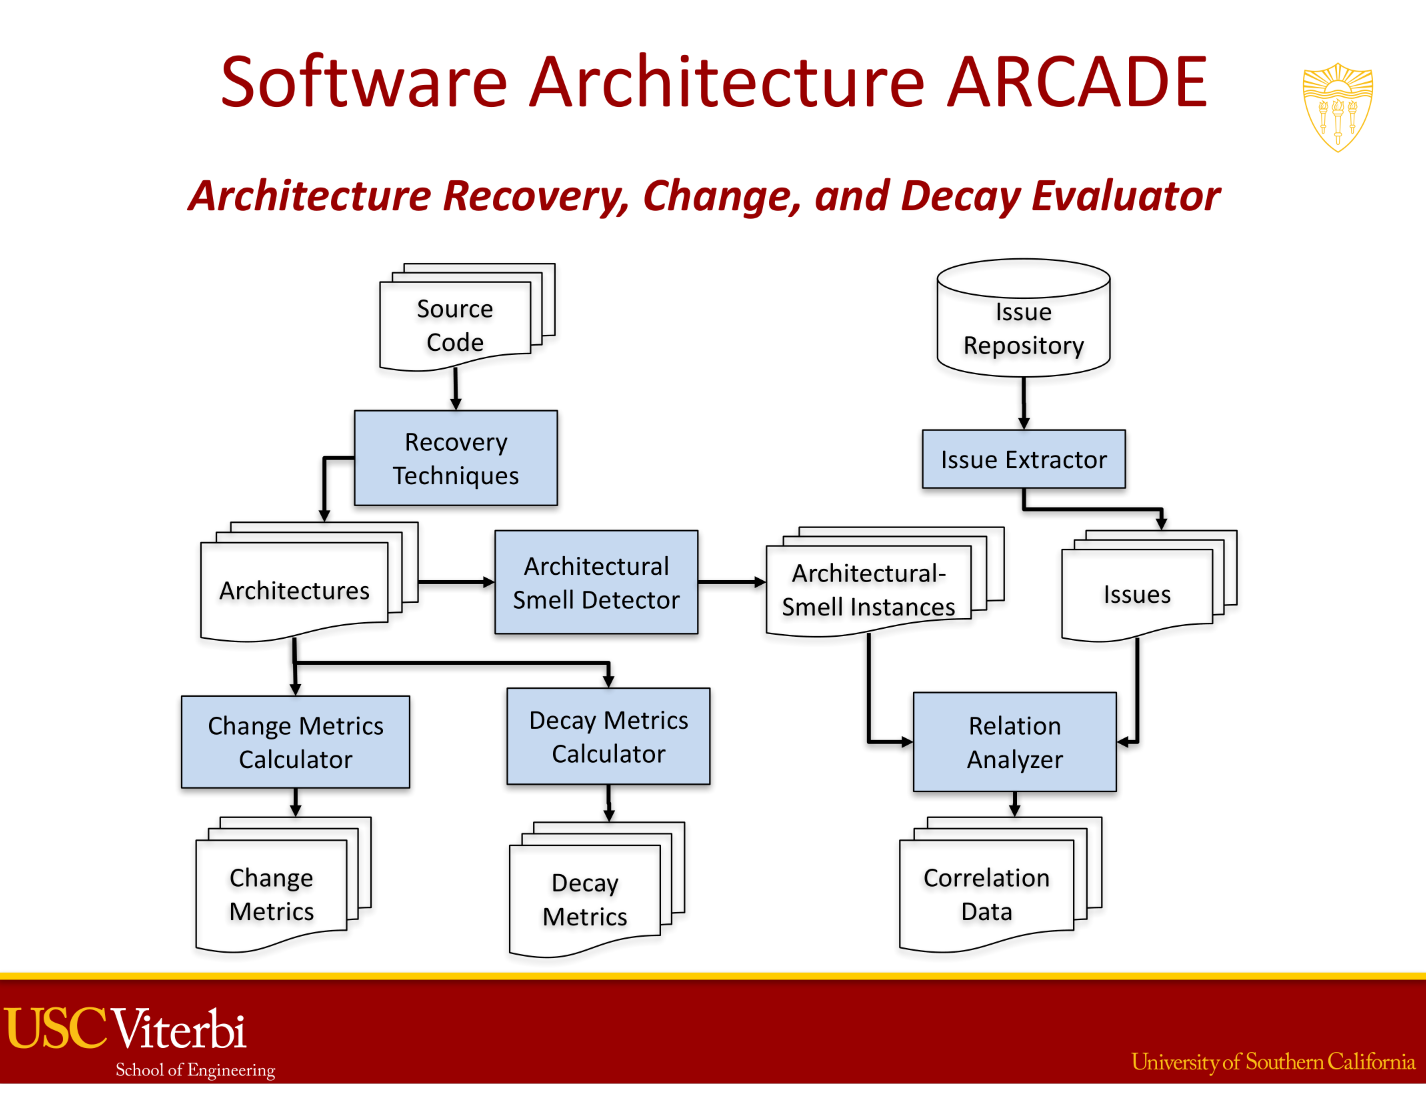
\includegraphics[width=0.9\textwidth]{medvidovic5.png}
		\end{center}
	\end{frame}

	\begin{frame}
		\begin{center}
			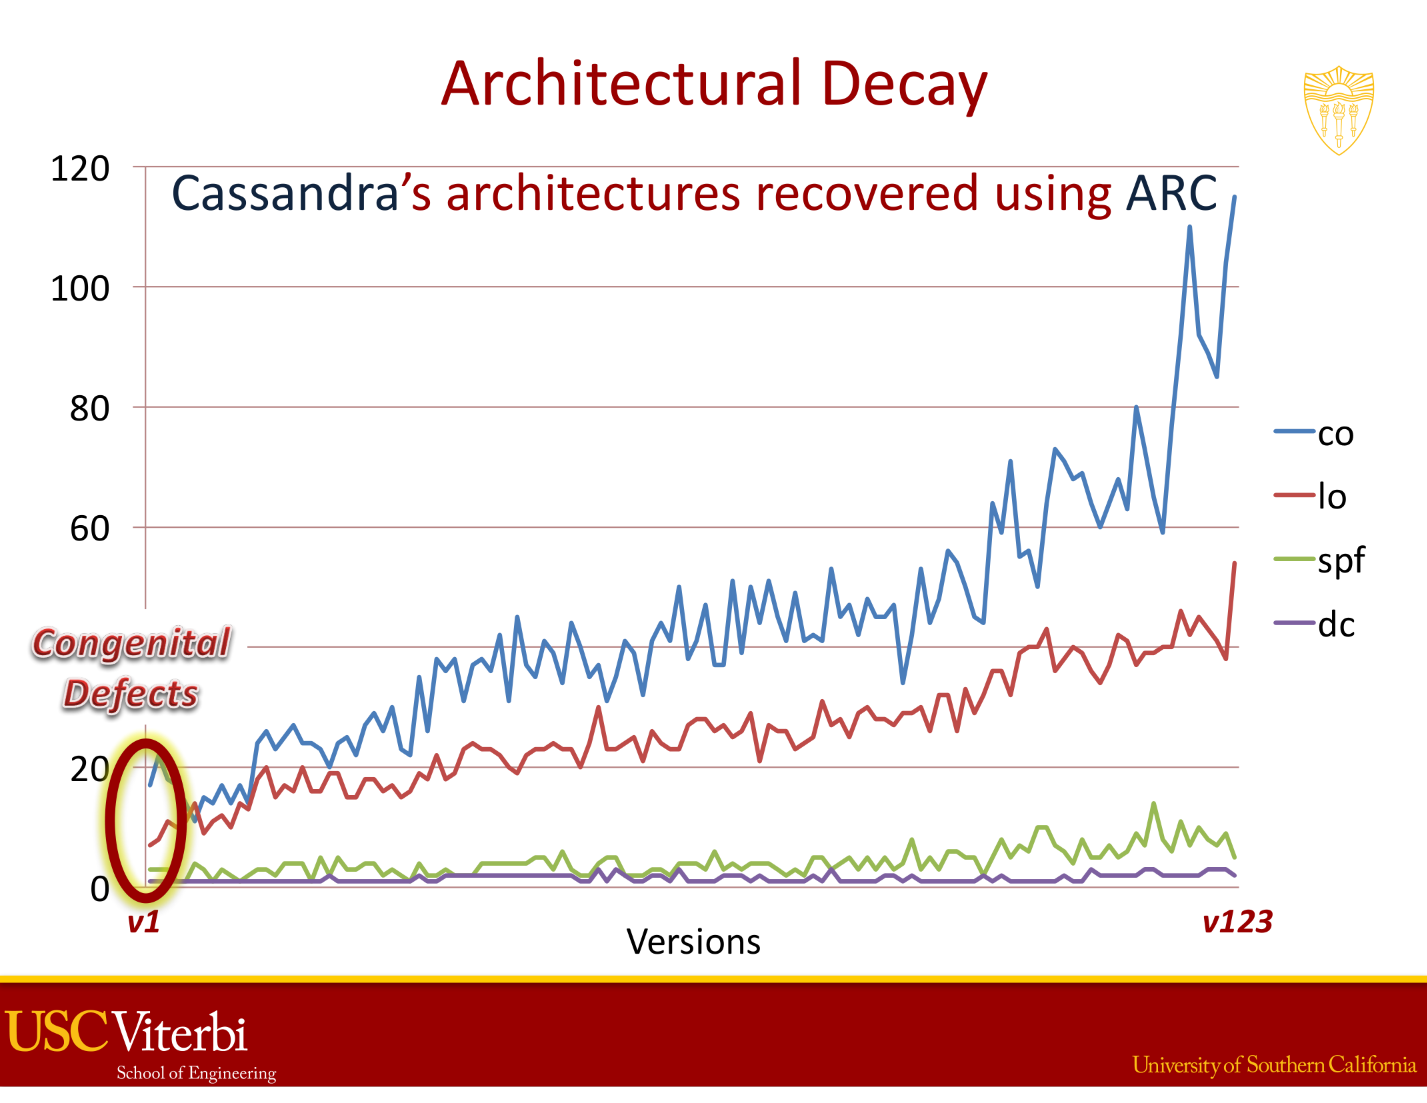
\includegraphics[width=0.9\textwidth]{medvidovic6.png}
		\end{center}
	\end{frame}

	\begin{frame}
		\begin{center}
			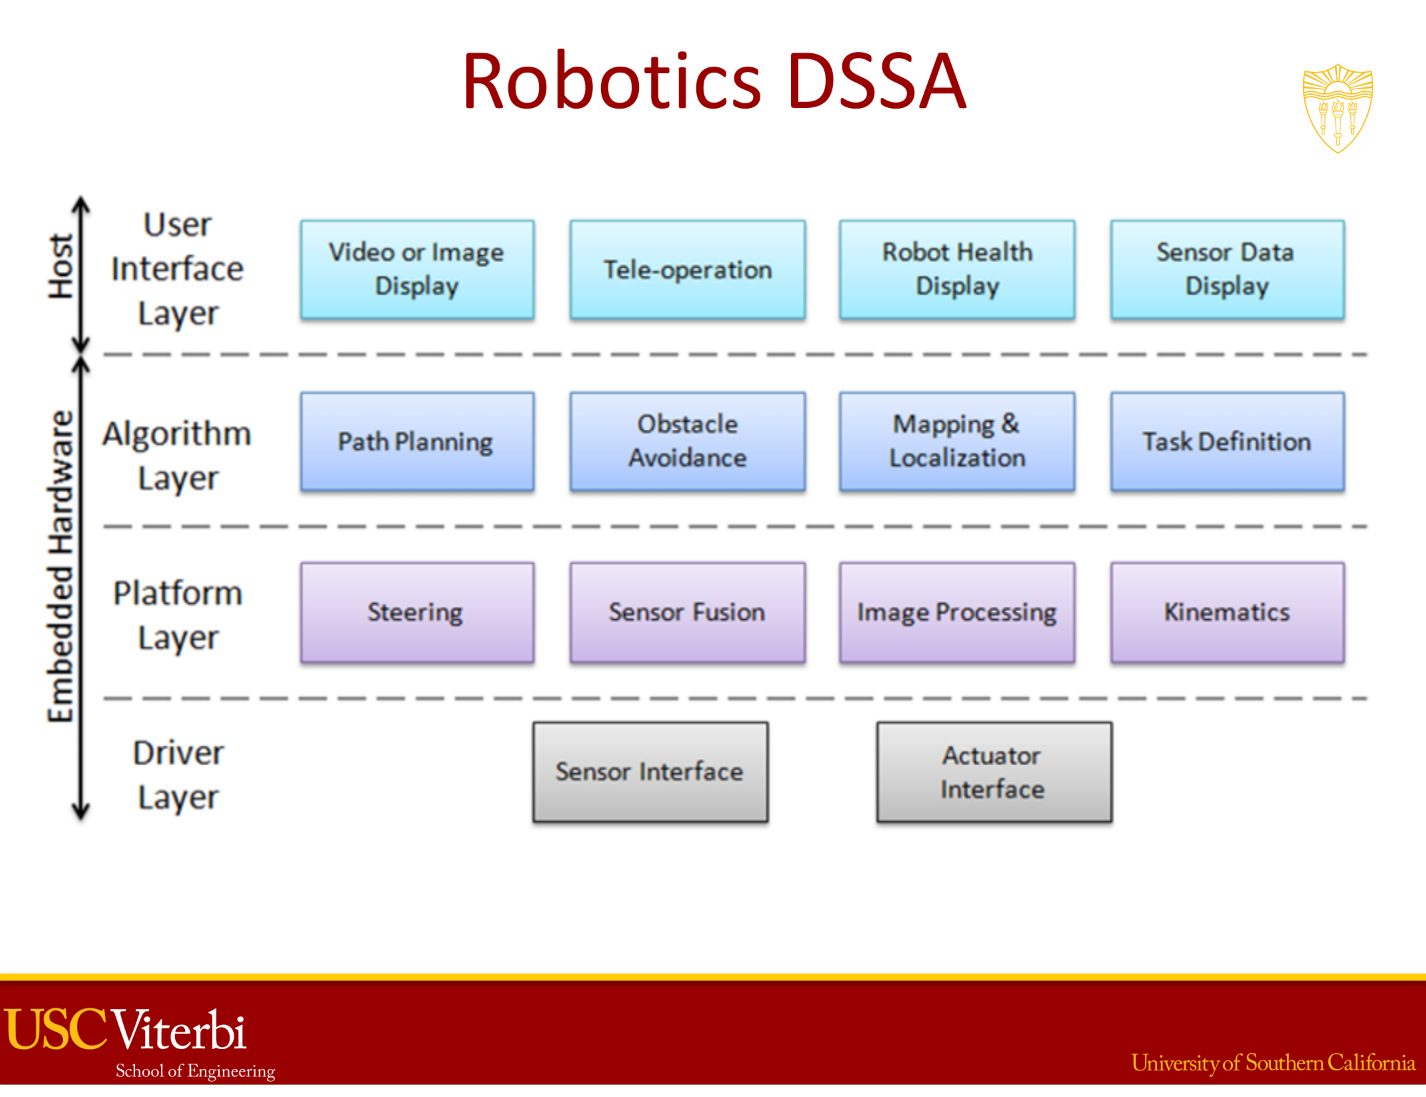
\includegraphics[width=0.9\textwidth]{medvidovic7.png}
		\end{center}
	\end{frame}

	\begin{frame}
		\begin{center}
			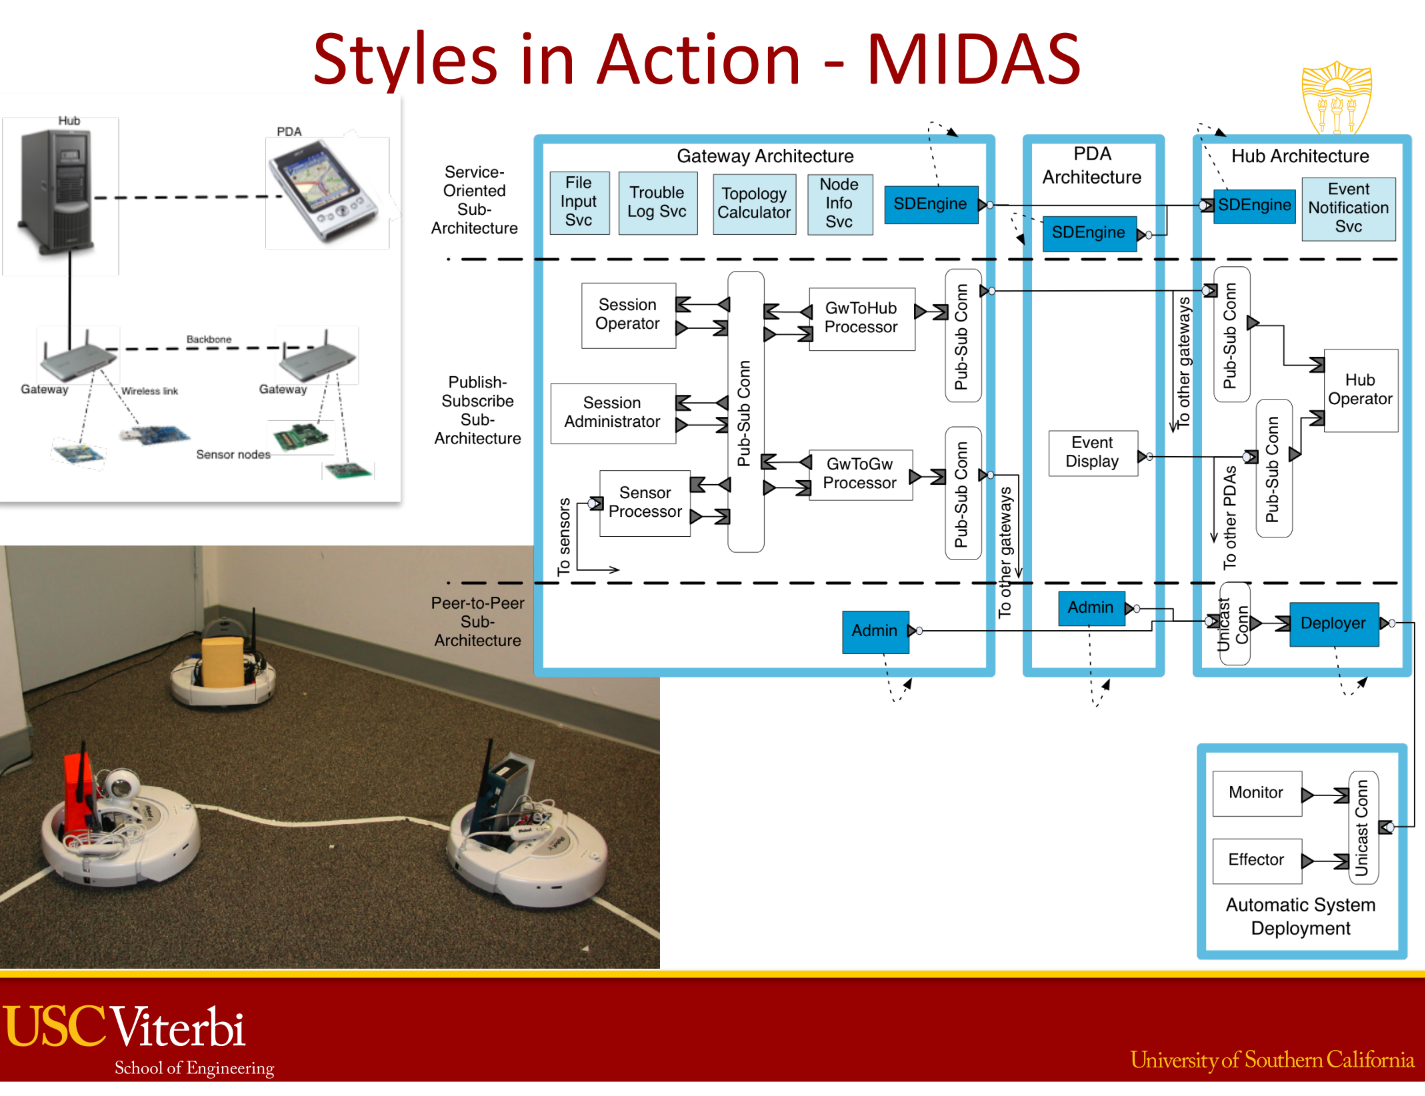
\includegraphics[width=0.9\textwidth]{medvidovic8.png}
		\end{center}
	\end{frame}

	\begin{frame}
		\begin{center}
			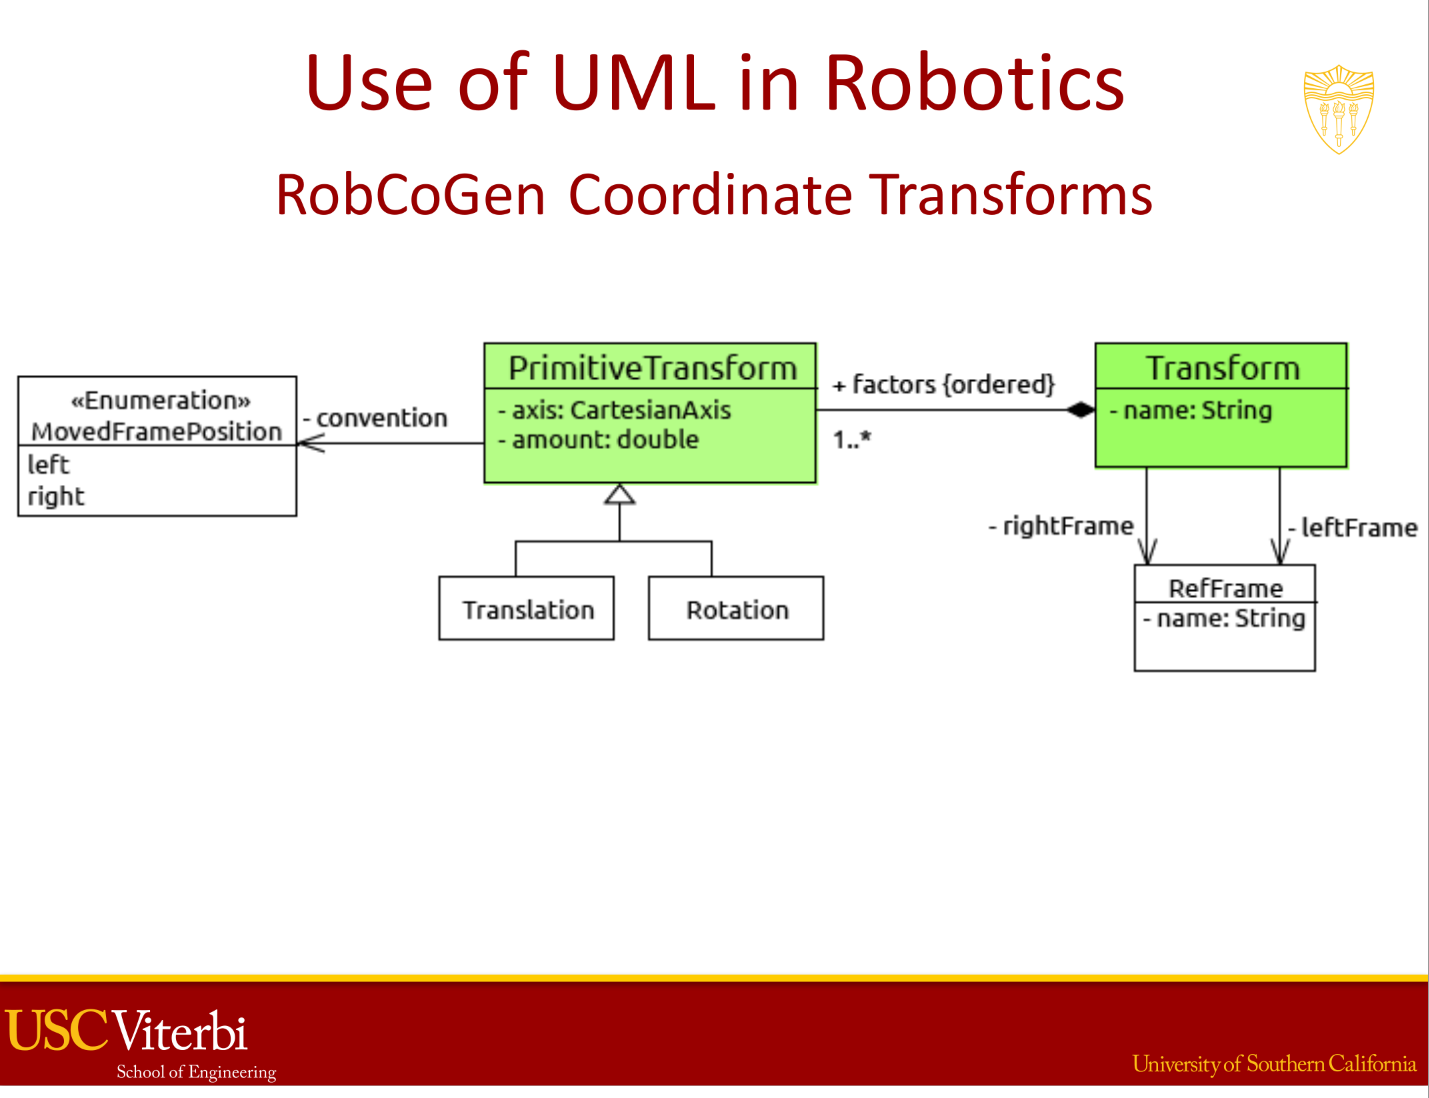
\includegraphics[width=0.9\textwidth]{medvidovic9.png}
		\end{center}
	\end{frame}

	\begin{frame}
		\begin{center}
			\includegraphics[width=0.9\textwidth]{medvidovic10.png}
		\end{center}
	\end{frame}

	\begin{frame}
		\begin{center}
			\includegraphics[width=0.9\textwidth]{medvidovic11.png}
		\end{center}
	\end{frame}

	\begin{frame}
		\begin{center}
			\includegraphics[width=0.9\textwidth]{medvidovic12.png}
		\end{center}
	\end{frame}

	\begin{frame}
		\begin{center}
			\includegraphics[width=0.9\textwidth]{medvidovic13.png}
		\end{center}
	\end{frame}

	\section{B. Meyer}

	\begin{frame}
		\begin{center}
			\includegraphics[width=0.9\textwidth]{meyer1.png}
		\end{center}
	\end{frame}

	\begin{frame}
		\begin{center}
			\includegraphics[width=0.9\textwidth]{meyer2.png}
		\end{center}
	\end{frame}

	\begin{frame}
		\begin{center}
			\includegraphics[width=0.9\textwidth]{meyer3.png}
		\end{center}
	\end{frame}

	\begin{frame}
		\begin{center}
			\includegraphics[width=0.9\textwidth]{meyer4.png}
		\end{center}
	\end{frame}

	\begin{frame}
		\begin{center}
			\includegraphics[width=0.9\textwidth]{meyer5.png}
		\end{center}
	\end{frame}

	\begin{frame}
		\begin{center}
			\includegraphics[width=0.9\textwidth]{meyer6.png}
		\end{center}
	\end{frame}

	\begin{frame}
		\begin{center}
			\includegraphics[width=0.9\textwidth]{meyer7.png}
		\end{center}
	\end{frame}

	\begin{frame}
		\begin{center}
			\includegraphics[width=0.9\textwidth]{meyer8.png}
		\end{center}
	\end{frame}

	\begin{frame}
		\begin{center}
			\includegraphics[width=0.9\textwidth]{meyer9.png}
		\end{center}
	\end{frame}

	\begin{frame}
		\begin{center}
			\includegraphics[width=0.9\textwidth]{meyer10.png}
		\end{center}
	\end{frame}

	\section{I. Nesnas}
	
	\begin{frame}
		\frametitle{Issa Nesnas}
		\begin{itemize}
			\item Не выложил слайды!
			\item Рассказывал в основном про навигацию мобильных роботов (роверов) и про архитектуру бортового ПО
		\end{itemize}
		\begin{center}
			\includegraphics[width=0.5\textwidth]{pathfinder.png}
		\end{center}
	\end{frame}

	\begin{frame}
		\begin{center}
			\includegraphics[width=0.9\textwidth]{visualTracker.png}
		\end{center}
	\end{frame}

	\section{H. Okuno}

	\begin{frame}
		\begin{center}
			\includegraphics[width=0.8\textwidth]{okuno1.png}
		\end{center}
	\end{frame}

	\begin{frame}
		\begin{center}
			\includegraphics[width=0.8\textwidth]{okuno2.png}
		\end{center}
	\end{frame}

	\begin{frame}
		\begin{center}
			\includegraphics[width=0.8\textwidth]{okuno3.png}
		\end{center}
	\end{frame}

	\begin{frame}
		\begin{center}
			\includegraphics[width=0.8\textwidth]{okuno4.png}
		\end{center}
	\end{frame}

	\begin{frame}
		\begin{center}
			\includegraphics[width=0.8\textwidth]{okuno5.png}
		\end{center}
	\end{frame}

	\begin{frame}
		\begin{center}
			\includegraphics[width=0.8\textwidth]{okuno6.png}
		\end{center}
	\end{frame}

	\begin{frame}
		\begin{center}
			\includegraphics[width=0.8\textwidth]{okuno7.png}
		\end{center}
	\end{frame}

	\begin{frame}
		\begin{center}
			\includegraphics[width=0.8\textwidth]{okuno8.png}
		\end{center}
	\end{frame}

	\begin{frame}
		\begin{center}
			\includegraphics[width=0.8\textwidth]{okuno9.png}
		\end{center}
	\end{frame}

	\begin{frame}
		\begin{center}
			\includegraphics[width=0.8\textwidth]{okuno10.png}
		\end{center}
	\end{frame}

	\begin{frame}
		\begin{center}
			\includegraphics[width=0.8\textwidth]{okuno11.png}
		\end{center}
	\end{frame}

	\begin{frame}
		\begin{center}
			\includegraphics[width=0.8\textwidth]{okuno12.png}
		\end{center}
	\end{frame}

	\begin{frame}
		\begin{center}
			\includegraphics[width=0.8\textwidth]{okuno13.png}
		\end{center}
	\end{frame}

	\begin{frame}
		\begin{center}
			\includegraphics[width=0.8\textwidth]{okuno14.png}
		\end{center}
	\end{frame}

	\begin{frame}
		\begin{center}
			\includegraphics[width=0.8\textwidth]{okuno15.png}
		\end{center}
	\end{frame}

	\begin{frame}
		\begin{center}
			\includegraphics[width=0.8\textwidth]{okuno16.png}
		\end{center}
	\end{frame}

	\begin{frame}
		\begin{center}
			\includegraphics[width=0.8\textwidth]{okuno17.png}
		\end{center}
	\end{frame}

	\begin{frame}
		\begin{center}
			\includegraphics[width=0.8\textwidth]{okuno18.png}
		\end{center}
	\end{frame}

	\begin{frame}
		\begin{center}
			\includegraphics[width=0.8\textwidth]{okuno19.png}
		\end{center}
	\end{frame}

	\begin{frame}
		\begin{center}
			\includegraphics[width=0.8\textwidth]{okuno20.png}
		\end{center}
	\end{frame}

	\begin{frame}
		\begin{center}
			\includegraphics[width=0.8\textwidth]{okuno21.png}
		\end{center}
	\end{frame}

	\begin{frame}
		\begin{center}
			\includegraphics[width=0.8\textwidth]{okuno22.png}
		\end{center}
	\end{frame}

	\begin{frame}
		\begin{center}
			\includegraphics[width=0.8\textwidth]{okuno23.png}
		\end{center}
	\end{frame}

\end{document}

